%% For double-blind review submission, w/o CCS and ACM Reference (max submission space)
\documentclass[format=acmsmall, screen=true,review,anonymous, nonacm,pdftex,svgnames]{acmart}
%% For double-blind review submission, w/ CCS and ACM Reference
%\documentclass[sigplan,review,anonymous]{acmart}\settopmatter{printfolios=true}
%% For single-blind review submission, w/o CCS and ACM Reference (max submission space)
%\documentclass[sigplan,review]{acmart}\settopmatter{printfolios=true,printccs=false,printacmref=false}
%% For single-blind review submission, w/ CCS and ACM Reference
%\documentclass[sigplan,review]{acmart}\settopmatter{printfolios=true}
%% For final camera-ready submission, w/ required CCS and ACM Reference
%\documentclass[sigplan]{acmart}\settopmatter{}


%% Conference information
%% Supplied to authors by publisher for camera-ready submission;
%% use defaults for review submission.
\acmJournal{PACMPL}
\acmVolume{1}
\acmNumber{OOPSLA} % CONF = POPL or ICFP or OOPSLA
\acmArticle{1}
\acmYear{2022}
\acmMonth{1}
\acmDOI{} % \acmDOI{10.1145/nnnnnnn.nnnnnnn}
\startPage{1}

%% Copyright information
%% Supplied to authors (based on authors' rights management selection;
%% see authors.acm.org) by publisher for camera-ready submission;
%% use 'none' for review submission.
\setcopyright{none}
%\setcopyright{acmcopyright}
%\setcopyright{acmlicensed}
%\setcopyright{rightsretained}
%\copyrightyear{2018}           %% If different from \acmYear

%% Bibliography style
\bibliographystyle{ACM-Reference-Format}
%% Citation style
%\citestyle{acmauthoryear}  %% For author/year citations
%\citestyle{acmnumeric}     %% For numeric citations
%\setcitestyle{nosort}      %% With 'acmnumeric', to disable automatic
                            %% sorting of references within a single citation;
                            %% e.g., \cite{Smith99,Carpenter05,Baker12}
                            %% rendered as [14,5,2] rather than [2,5,14].
%\setcitesyle{nocompress}   %% With 'acmnumeric', to disable automatic
                            %% compression of sequential references within a
                            %% single citation;
                            %% e.g., \cite{Baker12,Baker14,Baker16}
                            %% rendered as [2,3,4] rather than [2-4].

\citestyle{acmauthoryear}   %% For author/year citations
%%%%%%%%%%%%%%%%%%%%%%%%%%%%%%%%%%%%%%%%%%%%%%%%%%%%%%%%%%%%%%%%%%%%%%
%% Note: Authors migrating a paper from traditional SIGPLAN
%% proceedings format to PACMPL format must update the
%% '\documentclass' and topmatter commands above; see
%% 'acmart-pacmpl-template.tex'.
%%%%%%%%%%%%%%%%%%%%%%%%%%%%%%%%%%%%%%%%%%%%%%%%%%%%%%%%%%%%%%%%%%%%%%



%% Some recommended packages.
\usepackage{booktabs}   %% For formal tables:
                        %% http://ctan.org/pkg/booktabs
\usepackage{subcaption} %% For complex figures with subfigures/subcaptions
                        %% http://ctan.org/pkg/subcaption
\usepackage{bussproofs}
\usepackage[cal=boondoxo]{mathalfa}
\DeclareMathAlphabet{\mathpzc}{OT1}{pzc}{m}{it}
\usepackage{amsmath}
\newtheorem{theorem}{Theorem}[section]
\newtheorem{observation}[theorem]{Observation}
\usepackage{color}
\usepackage{xspace}
\newcommand{\comm}[3][\color{red}]{{#1{[{#2}: {#3}]}}}
%\newcommand{\comm}[3][\color{red}]{}
%\newcommand{\mwh}[1]{\comm[\color{blue}]{Mike}{#1}}

%\input{prooftree}

\newcommand{\ignore}[1]{{}}
\newcommand{\CTLK}{\textbf{CTLK}\xspace}
\newcommand{\TransK}{\textbf{TransK}\xspace}
\newcommand{\IsaK}{\textbf{IsaK}\xspace}
\newcommand{\IsaKa}{\textbf{IsaK+}\xspace}
\def\mcirc{\mathord{\scalebox{1.5}[1]{\scalerel*{\circ}{\strut}}}}
\def\msquare{\mathord{\scalerel*{\Box}{gX}}}
%\newcommand{\K}{\ensuremath{\mathbb{K}}\xspace}
\newcommand{\core}{\textbf{CORE}\xspace}
%\newcommand{\syntax}{\textbf{SYNTAX}\xspace}
\newcommand{\syntaxConstr}{\textbf{Syntax}\xspace}
\newcommand{\tokenConstr}{\textbf{Token}\xspace}
\newcommand{\subsortConstr}{\textbf{Subsort}\xspace}
\newcommand{\listSyntaxConstr}{\textbf{ListSyntax}\xspace}
\newcommand{\terminalConstr}{\textbf{Terminal}\xspace}
\newcommand{\nonterminalConstr}{\textbf{NonTerminal}\xspace}
\newcommand{\getStackType}{\texttt{getStackType}\xspace}
\newcommand{\gtop}{\texttt{top}\xspace}
\newcommand{\pick}{\texttt{pick}\xspace}
\newcommand{\match}{\texttt{match}\xspace}
\newcommand{\subst}{\texttt{subst}\xspace}
%\newcommand{\norm}{\texttt{norm}\xspace}
\newcommand{\typed}{\texttt{typed}\xspace}
\newcommand{\nelist}{\texttt{nelist}\xspace}
\newcommand{\genList}{\texttt{list}\xspace}
\newcommand{\genSet}{\texttt{set}\xspace}
\newcommand{\genLists}{\texttt{lists}\xspace}
\newcommand{\astring}{\texttt{string}\xspace}
\newcommand{\regex}{\texttt{regex}\xspace}
\newcommand{\theSymbol}{\texttt{symbol}\xspace}
\newcommand{\sortId}{\texttt{sortId}\xspace}
\newcommand{\cellId}{\texttt{cellId}\xspace}
\newcommand{\metaId}{\texttt{metaId}\xspace}
\newcommand{\labelId}{\texttt{labelId}\xspace}
\newcommand{\ir}{\textbf{IR}\xspace}
\newcommand{\cool}{\texttt{cool}\xspace}
\newcommand{\forname}{\constant{forname}\;}
\newcommand{\kif}{\constant{if}\;}
\newcommand{\kthen}{\constant{then}\;}
\newcommand{\kelse}{\constant{else}\;}
\newcommand{\kskip}{\constant{skip}\;}
\newcommand{\loopin}{\constant{in}\;}
\newcommand{\heat}{\texttt{heat}\xspace}
\newcommand{\kCell}{\texttt{kCell}\xspace}
\newcommand{\KResult}{\texttt{KResult}\xspace}
\newcommand{\kSyntax}{\texttt{kSyntax}\xspace}
\newcommand{\syntaxDef}[3]{\rulebox{%
\syntaxKeyword$#1\mathrel{::=}{#2}$ \ifthenelse{\equal{#3}{}}{}{[#3]}%
}%
}
\newcommand{\kvariable}[2]{\variable{#1}:\variable{#2}}
\newcommand{\kRule}{\texttt{kRule}\xspace}
\newcommand{\kRules}{\texttt{kRules}\xspace}
\newcommand{\irKRule}{\texttt{irKRule}\xspace}
\newcommand{\irKRules}{\texttt{irKRules}\xspace}
\newcommand{\kFile}{\texttt{kFile}\xspace}
\makeatletter
\newcommand{\shorteq}{%
  \settowidth{\@tempdima}{-}% Width of hyphen
  \resizebox{\@tempdima}{\height}{=}%
}
\makeatother


\newcommand{\RuleLabel}{\textit{RuleLabel}\xspace}
\newcommand{\RuleLabels}{\textit{RuleLabels}\xspace}
\newcommand{\QuestionKey}{\mathbf{?}\xspace}
\newcommand{\StarKey}{\mathbf{*}\xspace}
\newcommand{\Stream}{\textbf{Stream}\xspace}
\newcommand{\stdWord}{\texttt{std}\xspace}
\newcommand{\Multiplicity}{\textbf{Multiplicity}\xspace}
\newcommand{\keyWord}{\texttt{key}\xspace}
\newcommand{\feature}{\texttt{feature}\xspace}
\newcommand{\Context}{\textbf{Context}\xspace}
\newcommand{\Fun}{\textbf{Fun}\xspace}
\newcommand{\FunRule}{\textbf{FunRule}\xspace}
\newcommand{\FunRules}{\textbf{FunRules}\xspace}
\newcommand{\Macro}{\textbf{Macro}\xspace}
\newcommand{\MacroRule}{\textbf{MacroRule}\xspace}
\newcommand{\MacroRules}{\textbf{MacroRules}\xspace}
\newcommand{\Anywhere}{\textbf{Anywhere}\xspace}
\newcommand{\AnywhereRule}{\textbf{AnywhereRule}\xspace}
\newcommand{\AnywhereRules}{\textbf{AnywhereRules}\xspace}
\newcommand{\KNormal}{\textbf{KNormal}\xspace}
\newcommand{\KNormalRule}{\textbf{KNormalRule}\xspace}
\newcommand{\KNormalRules}{\textbf{KNormalRules}\xspace}
\newcommand{\BagNormal}{\textbf{BagNormal}\xspace}
\newcommand{\BagNormalRule}{\textbf{BagNormalRule}\xspace}
\newcommand{\BagNormalRules}{\textbf{BagNormalRules}\xspace}
\newcommand{\synAttr}{\texttt{synAttrib}\xspace}
\newcommand{\ruleAttr}{\texttt{ruleAttrib}\xspace}
\newcommand{\synAttrs}{\texttt{synAttribs}\xspace}
\newcommand{\ruleAttrs}{\texttt{ruleAttribs}\xspace}
\newcommand{\Strict}{\texttt{Strict}\xspace}
\newcommand{\productions}{\texttt{productions}\xspace}
\newcommand*{\Leadsto}{\ensuremath{\leadsto}\xspace}
\newcommand{\bigK}{\texttt{bigK}\xspace}
\newcommand{\bigKBag}{\texttt{bigKBag}\xspace}
\newcommand{\constType}{\texttt{const}\xspace}
\newcommand{\kLabel}{\texttt{kLabel}\xspace}
\newcommand{\kLabels}{\texttt{kLabels}\xspace}
\newcommand{\irPat}{\texttt{irFunPat}\xspace}
\newcommand{\irFunApp}{\texttt{irFunApp}\xspace}
\newcommand{\funApp}{\texttt{funApp}\xspace}
\newcommand{\irKLabel}{\texttt{irKLabel}\xspace}
\newcommand{\irKLabels}{\texttt{irKLabels}\xspace}
\newcommand{\kItem}{\texttt{kItem}\xspace}
\newcommand{\kItems}{\texttt{kItems}\xspace}
\newcommand{\irKItem}{\texttt{irKItem}\xspace}
\newcommand{\irKItems}{\texttt{irKItems}\xspace}
\newcommand{\irBigKBag}{\texttt{irBigKBag}\xspace}
\newcommand{\irBigKBagLabel}{\texttt{irBigKBagLabel}\xspace}
\newcommand{\kList}{\texttt{kList}\xspace}
\newcommand{\kLists}{\texttt{kLists}\xspace}
\newcommand{\irKListElem}{\texttt{irKListElem}\xspace}
\newcommand{\irKList}{(\texttt{irKListElem\;\genList})\xspace}
\newcommand{\irKLists}{(\texttt{irKListElem\;\genLists})\xspace}
\newcommand{\ak}{\texttt{k}\xspace}
\newcommand{\aks}{\texttt{ks}\xspace}
\newcommand{\irKElem}{\texttt{irKElem}\xspace}
\newcommand{\irK}{(\texttt{irKElem\;\genList})\xspace}
\newcommand{\irKs}{(\texttt{irKElem\;\genLists})\xspace}
\newcommand{\alist}{\texttt{aList}\xspace}
\newcommand{\alists}{\texttt{aLists}\xspace}
\newcommand{\irListElem}{\texttt{irListElem}\xspace}
\newcommand{\irList}{(\texttt{irListElem\xspace\genList})\xspace}
\newcommand{\irLists}{(\texttt{irListElem\xspace\genLists})\xspace}
\newcommand{\set}{\texttt{set}\xspace}
\newcommand{\sets}{\texttt{sets}\xspace}
\newcommand{\irSetElem}{\texttt{irSetElem}\xspace}
\newcommand{\irSet}{(\texttt{irSetElem\;\genList})\xspace}
\newcommand{\irSets}{(\texttt{irSetElem\;\genLists})\xspace}
\newcommand{\map}{\texttt{map}\xspace}
\newcommand{\maps}{\texttt{maps}\xspace}
\newcommand{\irMapElem}{\texttt{irMapElem}\xspace}
\newcommand{\irMap}{(\texttt{irMapElem\;\genList})\xspace}
\newcommand{\irMaps}{(\texttt{irMapElem\;\genLists})\xspace}
\newcommand{\cell}{\texttt{cell}\xspace}
\newcommand{\cells}{\texttt{cells}\xspace}
\newcommand{\bag}{\texttt{bag}\xspace}
\newcommand{\bags}{\texttt{bags}\xspace}
\newcommand{\irBagElem}{\texttt{irBagElem}\xspace}
\newcommand{\irBag}{(\texttt{irBagElem\;\genList})\xspace}
\newcommand{\irBags}{(\texttt{irBagElem\;\genLists})\xspace}
\newcommand{\rewrite}{\texttt{rewrite}\xspace}
\newcommand{\rewriteConstr}{\textbf{Rewrite}\xspace}
\newcommand{\rewriteConstrs}{\textbf{Rewrites}\xspace}
\newcommand{\program}{\texttt{program}\xspace}
\newcommand{\kompile}{\textbf{\textit{kompile}}\xspace}
\newcommand{\krun}{\textbf{\textit{krun}}\xspace}
\newcommand{\ksearch}{\textbf{\textit{ksearch}}\xspace}
\newcommand{\ktheory}{\ensuremath{\mathbb{K}}\texttt{\_theory}\xspace}

\newcommand{\genKLabel}{\texttt{genKLabel}\xspace}
\newcommand{\regexPar}{\texttt{regexPar}\xspace}

\newcommand{\kLabelSort}{\texttt{KLabel}\xspace}
\newcommand{\kItemSort}{\texttt{KItem}\xspace}
\newcommand{\kListSort}{\texttt{KList}\xspace}
\newcommand{\kSort}{\texttt{K}\xspace}
\newcommand{\listSort}{\texttt{List}\xspace}
\newcommand{\setSort}{\texttt{Set}\xspace}
\newcommand{\mapSort}{\texttt{Map}\xspace}
\newcommand{\bagSort}{\texttt{Bag}\xspace}

\newcommand{\topSort}{\texttt{topSort}\xspace}
\newcommand{\KItemIR}{\textbf{KItemIR}\xspace}
\newcommand{\IdKItemIR}{\textbf{IdKItemIR}\xspace}
\newcommand{\HOLEIR}{\textbf{HOLEIR}\xspace}
\newcommand{\KListElemIR}{\textbf{KListElemIR}\xspace}
\newcommand{\KListIdIR}{\textbf{KListIdIR}\xspace}
\newcommand{\strict}{\texttt{strict}\xspace}
\newcommand{\seqstrict}{\texttt{seqstrict}\xspace}
%\newcommand{\function}{\texttt{function}\xspace}
\newcommand{\klabelAttr}{\textbf{Klabel}\xspace}
\newcommand{\macroAttr}{\texttt{macro}\xspace}
\newcommand{\anywhereAttr}{\texttt{anywhere}\xspace}
\newcommand{\owiseAttr}{\textbf{Owise}\xspace}
\newcommand{\Transition}{\texttt{Transition}\xspace}
\newcommand{\transition}{\texttt{transition}\xspace}
\newcommand{\add}{\texttt{add}\xspace}
\newcommand{\hasFunTerm}{\texttt{hasFunTerm}\xspace}
\newcommand{\funMatch}{\texttt{funMatch}\xspace}
\newcommand{\kNormMatch}{\texttt{kNormMatch}\xspace}
\newcommand{\bagNormMatch}{\texttt{bagNormMatch}\xspace}
\newcommand{\anywhereMatch}{\texttt{anywhereMatch}\xspace}
\newcommand{\macroMatch}{\texttt{macroMatch}\xspace}
\newcommand{\sortAdjust}{\texttt{sortAdjust}\xspace}
\newcommand{\validMacroRules}{\texttt{validMacroRules}\xspace}
\newcommand{\getKLabel}{\texttt{getKLabel}\xspace}
\newcommand{\isFunLabel}{\texttt{isFunLabel}\xspace}
\newcommand{\cut}{\texttt{split}\xspace}
\newcommand{\compile}{\texttt{compile}\xspace}
\newcommand{\sortOf}{\texttt{sortOf}\xspace}
\newcommand{\argSortsOf}{\texttt{argSortsOf}\xspace}
\newcommand{\smallestSort}{\texttt{smallestSort}\xspace}
%\newcommand{\send}[3]{\textsf{!}[#1|#2]\to#3}

\newcommand{\letin}[3]{{\ensuremath{\textsf{let}\;{#1}={#2}\;\textsf{in}\;{#3}}}}
%[|(#2,#3)|#4|]#5
%% \newcommand{\bigparallels}[5]{{\ensuremath{
%% \begin{array}[t]{l}
%% #1\\
%%  |\![\!\{#2.#3|#4\}\!]\!|\\
%% #5
%% \end{array}}}}
\newcommand{\bigparallels}[5]{{\ensuremath{#1 |\![\!\{#2.#3|#4\}\!]\!|#5}}}
\newcommand{\seque}[2]{#1;#2}
\newcommand{\extchoices}[2]{#1\Box#2}
%\newcommand{\intchoices}[2]{#1|\sim|#2}
\newcommand{\intchoices}[2]{#1\sqcap#2}
\newcommand{\hiding}[4]{#1\setminus\{#2.#3|#4\}}
\newcommand{\rename}[6]{#1\;\ensuremath{[\![\!\{((#2.#3),(#4.#5))|#6\}\!]\!]}}
\newcommand{\WT}[1]{\textsf{Wf}(\textsf{#1})}

\newcommand{\LOGICAND}{{\textsf{Conjunction}}}
\newcommand{\LOGICOR}{{\textsf{Disjunction}}}
\newcommand{\LOGICNOT}{{\textsf{Negation}}}
\newcommand{\WELLTYPE}{{\textsf{Well-formed}}}
\newcommand{\EQUALITY}{{\textsf{Equality}}}
\newcommand{\WEAKENLOGICOR}{{\textsf{Strong-disjunction}}}
\newcommand{\WEAKENLOGICNOT}{{\textsf{Strong-negation}}}


\newcommand{\reglai}[3]{
    \prooftree
         #1
    \justifies  
         #2
    \thickness=0.05em
    \using
        #3
    \endprooftree}

\newcommand{\reglaii}[4]{
    \prooftree
         #1\quad
         #2
    \justifies  
         #3
    \thickness=0.05em
    \using
        #4
    \endprooftree}

\newcommand{\sreglai}[3]{
    \prooftree
\begin{array}{c}
         #1
\end{array}
    \justifies  
         #2
    \thickness=0.05em
    \using
        #3
    \endprooftree}


\newcommand{\sreglaii}[4]{
    \prooftree
\begin{array}{c}
         #1\\
         #2
\end{array}
    \justifies  
         #3
    \thickness=0.05em
    \using
        #4
    \endprooftree}

\newcommand{\sreglaiii}[5]{
    \prooftree
\begin{array}{c}
         #1\\
         #2\\
	 #3
\end{array}
    \justifies  
         #4
    \thickness=0.05em
    \using
        #5
    \endprooftree}

\newcommand{\ssregla}[6]{
    \prooftree
\begin{array}{c}
         #1\\[-.7em]
         #2\\[-.7em]
	 #3\\[-.7em]
	 #4
\end{array}
    \justifies  
         #5
    \thickness=0.05em
    \using
        #6
    \endprooftree}


\newcommand{\reglaiii}[5]{
    \prooftree
         #1\quad
         #2\quad
         #3
    \justifies  
         #4
    \thickness=0.05em
    \using
        #5
    \endprooftree}

\newcommand{\reglaiv}[6]{
    \prooftree
         #1\quad
         #2\quad
         #3\quad
         #4
    \justifies  
         #5
    \thickness=0.05em
    \using
        #6
    \endprooftree}


\newcommand{\pist}{\ensuremath{\mathsf{Iris}}}

% Process terms
\newcommand{\chIn}[3]{\ensuremath{#1?(#2)\ \texttt{in}\ #3}}
\newcommand{\chOut}[2]{\ensuremath{#1![#2]}}
\newcommand{\palel}[2]{#1\ensuremath{|}\,#2}
\newcommand{\branch}{\ensuremath{\rhd}\,}
\newcommand{\select}{\ensuremath{\lhd}\,}
\newcommand{\new}[2]{\ensuremath{(\nu #1)#2}}
\newcommand{\inicioAss}[1]{\ensuremath{\texttt{begin}\ #1}}
\newcommand{\finAss}[1]{\ensuremath{\texttt{end}\ #1}}
\newcommand{\accept}[2]{\ensuremath{\texttt{accept}\ #1\ \texttt{in}\ #2}}
\newcommand{\request}[2]{\ensuremath{\texttt{request}\ #1\ \texttt{in}\ #2}}
\newcommand{\throw}[2]{\ensuremath{\texttt{throw}\ #1[#2]}}
\newcommand{\catch}[3]{\ensuremath{\texttt{catch}\ #1(#2)\ \texttt{in}\ #3}}
\newcommand{\defin}[2]{\ensuremath{\texttt{def}\ #1\ \texttt{in}\ #2}}
%\newcommand{\zero}{\ensuremath{\texttt{stop}}}
\newcommand{\callProc}[2]{\ensuremath{#1[#2]}}
\newcommand{\declProc}[3]{\ensuremath{#1[#2]=#3}}


% ATM example
\newcommand{\Atm}{\ensuremath{\textsf{ATM}}}
\newcommand{\Atmi}{\ensuremath{\textsf{ATM'}}}
\newcommand{\Atmii}{\ensuremath{\textsf{ATM''}}}
\newcommand{\Bank}{\ensuremath{\textsf{Bank}}}
\newcommand{\Client}{\ensuremath{\textsf{Client}}}
\newcommand{\Clienti}{\ensuremath{\textsf{Client'}}}
\newcommand{\Banki}{\ensuremath{\textsf{Bank'}}}
\newcommand{\atmDef}[1]{\ensuremath{\textsf{ATM}(#1)}}
\newcommand{\atmCall}[1]{\ensuremath{\textsf{ATM}[#1]}}
\newcommand{\bankDef}[1]{\ensuremath{\textsf{Bank}(#1)}}
\newcommand{\bankCall}[1]{\ensuremath{\textsf{Bank}[#1]}}
\newcommand{\clientDef}[1]{\ensuremath{\textsf{Client}(#1)}}
\newcommand{\clientCall}[1]{\ensuremath{\textsf{Client}[#1]}}

% Auction example
\newcommand{\Auctioneer}{\ensuremath{\textsf{Auctioneer}}}
\newcommand{\InitAuctioneer}{\ensuremath{\textsf{InitAuctioneer}}}
\newcommand{\Buyer}{\ensuremath{\textsf{Buyer}}}
\newcommand{\InitBuyerManager}{\ensuremath{\textsf{InitBuyerManager}}}
\newcommand{\BuyerManager}{\ensuremath{\textsf{BuyerManager}}}
\newcommand{\Seller}{\ensuremath{\textsf{Seller}}}
\newcommand{\InitSellerManager}{\ensuremath{\textsf{InitSellerManager}}}
\newcommand{\SellerManager}{\ensuremath{\textsf{SellerManager}}}
\newcommand{\BuyerDef}[3]{\ensuremath{\textsf{Buyer}(#1,#2,#3)}}
\newcommand{\SellerDef}[3]{\ensuremath{\textsf{Seller}(#1,#2,#3)}}
\newcommand{\AuctioneerDef}[3]{\ensuremath{\textsf{Auctioneer}(#1,#2,#3)}}
\newcommand{\InitAuctioneerDef}[3]{\ensuremath{\textsf{InitAuctioneer}(#1,#2,#3)}}
\newcommand{\InitBuyerManagerDef}[2]{\ensuremath{\textsf{InitBuyerManager}(#1,#2)}}
\newcommand{\BuyerManagerDef}[4]{\ensuremath{\textsf{BuyerManager}(#1,#2,#3,#4)}}
\newcommand{\InitSellerManagerDef}[2]{\ensuremath{\textsf{InitSellerManager}(#1,#2)}}
\newcommand{\SellerManagerDef}[2]{\ensuremath{\textsf{SellerManager}(#1,#2)}}
\newcommand{\BuyerCall}[3]{\ensuremath{\textsf{Buyer}[#1,#2,#3]}}
\newcommand{\SellerCall}[3]{\ensuremath{\textsf{Seller}[#1,#2,#3]}}
\newcommand{\AuctioneerCall}[3]{\ensuremath{\textsf{Auctioneer}[#1,#2,#3]}}
\newcommand{\InitAuctioneerCall}[3]{\ensuremath{\textsf{InitAuctioneer}[#1,#2,#3]}}
\newcommand{\InitBuyerManagerCall}[2]{\ensuremath{\textsf{InitBuyerManager}[#1,#2]}}
\newcommand{\BuyerManagerCall}[4]{\ensuremath{\textsf{BuyerManager}[#1,#2,#3,#4]}}
\newcommand{\InitSellerManagerCall}[2]{\ensuremath{\textsf{InitSellerManager}[#1,#2]}}
\newcommand{\SellerManagerCall}[2]{\ensuremath{\textsf{SellerManager}[#1,#2]}}


% Types

%\newcommand{\name}{\mathbf{Name}}
\newcommand{\intType}{\ensuremath{\mathbf{Int}}}
\newcommand{\msg}[1]{\ensuremath{\langle #1\rangle}}   % message
\newcommand{\branchType}[2]{\ensuremath{\&\{#1\}#2}}     % branch type
\newcommand{\selectType}[2]{\ensuremath{\oplus\{#1\}#2}} % select type
\newcommand{\effects}[1]{\ensuremath{(\!\mid\!#1\!\mid\!)}}  % mult-set effects
\newcommand{\labl}[1]{\ensuremath{\langle #1\rangle}}

\newcommand{\chInType}[2]{\ensuremath{\downarrow[#1]#2}}
\newcommand{\chOutType}[2]{\ensuremath{\uparrow[#1]#2}}
\newcommand{\chInOutType}[2]{\ensuremath{\updownarrow[#1]#2}}
\newcommand{\dual}[1]{\ensuremath{\overline{#1}}}
\newcommand{\sessType}[1]{\ensuremath{\sigma(#1)}}
%\newcommand{\noConnection}{\ensuremath{\mathbf{\perp}}}
\newcommand{\noConnection}[1]{\ensuremath{\mathbf{\perp}_{#1}}}

\newcommand{\finConnection}{\ensuremath{\mathbf{1}}}
\newcommand{\recType}[2]{\ensuremath{\mu #1.#2}}


% Semantics

\newcommand{\congr}{\ensuremath{\equiv}}
%\newcommand{\redAc}[1]{\ensuremath{\stackrel{{\footnotesize #1}}{\longrightarrow}}}
\newcommand{\redAc}[1]{\ensuremath{\stackrel{{
\mbox{\footnotesize\ensuremath{#1} } }}{\longrightarrow}}}
\newcommand{\silent}{\ensuremath{\tau}}
\newcommand{\gen}[1]{\ensuremath{\mathtt{res}(#1)}}
\newcommand{\inicios}[1]{\ensuremath{\texttt{begins}(#1)}}
\newcommand{\fins}[1]{\ensuremath{\texttt{ends}(#1)}}
\newcommand{\genaction}{\psi}

% Wf types and channels - Rule Names

\newcommand{\wfNilEnv}{\ensuremath{\textsf{Wf Env Nil}}}
\newcommand{\wfConsTypeEnv}{\ensuremath{\textsf{Wf Env ConsT}}}
\newcommand{\wfConsChanEnv}{\ensuremath{\textsf{Wf Env ConsChT}}}

\newcommand{\wfBranch}{\ensuremath{\textsf{Wf Brnch}}}
\newcommand{\wfSelect}{\ensuremath{\textsf{Wf Sel}}}
\newcommand{\wfInOutType}{\ensuremath{\textsf{Wf In/Out}}}
\newcommand{\wfInOutChType}{\ensuremath{\textsf{Wf Ch In/Out}}}

\newcommand{\wfNilEffect}{\ensuremath{\textsf{Wf Eff Nil}}}
\newcommand{\wfConsEffect}{\ensuremath{\textsf{Wf Eff Cons}}}
\newcommand{\wfTypeVar}{\ensuremath{\textsf{Wf Env TVar}}}
\newcommand{\wfChanTypeVar}{\ensuremath{\textsf{Wf Env ChTVar}}}
\newcommand{\wfRecType}{\ensuremath{\textsf{Wf Rec Type}}}
\newcommand{\wfRecChan}{\ensuremath{\textsf{Wf Rec Chan}}}
\newcommand{\wfProcessVar}{\ensuremath{\textsf{Wf PVar}}}

\newcommand{\wfIntType}{\ensuremath{\textsf{Wf Int Type}}}
\newcommand{\wfUnitChannel}{\ensuremath{\textsf{Wf Unit ChT}}}
\newcommand{\wfEndChannel}{\ensuremath{\textsf{Wf End ChT}}}
\newcommand{\wfBulletChannel}{\ensuremath{\textsf{Wf No Comm}}}
\newcommand{\wfSessionType}{\ensuremath{\textsf{Wf Sess Type}}}


\newcommand{\wfProcessParamNil}{\ensuremath{\textsf{Wf PP Nil}}}
\newcommand{\wfProcessParamCons}{\ensuremath{\textsf{Wf PP Cons}}}

% Type System - Rule Names


\newcommand{\typeChan}{\ensuremath{\textsf{Type Chan}}}
\newcommand{\typeAccept}{\ensuremath{\textsf{Type Acpt}}}
\newcommand{\typeRequest}{\ensuremath{\textsf{Type Requ}}}
\newcommand{\typeSubsum}{\ensuremath{\textsf{Type Subsum}}}
\newcommand{\typeSend}{\ensuremath{\textsf{Type Snd}}}
\newcommand{\typeReceive}{\ensuremath{\textsf{Type Rcv}}}
\newcommand{\typeSelect}{\ensuremath{\textsf{Type Sel}}}
\newcommand{\typeBranch}{\ensuremath{\textsf{Type Brnch}}}
\newcommand{\typePar}{\ensuremath{\textsf{Type Par}}}
\newcommand{\typeThrow}{\ensuremath{\textsf{Type Thr}}}
\newcommand{\typeCatch}{\ensuremath{\textsf{Type Cat}}}
\newcommand{\typeBegin}{\ensuremath{\textsf{Type Bgn}}}
\newcommand{\typeEnd}{\ensuremath{\textsf{Type End}}}
\newcommand{\typeNameRes}{\ensuremath{\textsf{Type NRes}}}
\newcommand{\typeChanRes}{\ensuremath{\textsf{Type CRes}}}
\newcommand{\typeStop}{\ensuremath{\textsf{Type Stop}}}
\newcommand{\typeMsgNil}{\ensuremath{\textsf{Msg Nil}}}
\newcommand{\typeMsgCons}{\ensuremath{\textsf{Msg Cons}}}

\newcommand{\wfValueName}{\ensuremath{\textsf{Wf Val EName}}}
\newcommand{\wfValueInt}{\ensuremath{\textsf{Wf Val Int}}}

\newcommand{\typeProcessVar}{\ensuremath{\textsf{Type PVar}}}
\newcommand{\typeDefinition}{\ensuremath{\textsf{Type Def}}}

% Semantics - Structural Congruence

\newcommand{\scRefl}{\ensuremath{\textsf{SC Refl}}}
\newcommand{\scSymm}{\ensuremath{\textsf{SC Symm}}}
\newcommand{\scTrans}{\ensuremath{\textsf{SC Trans}}}
\newcommand{\scStop}{\ensuremath{\textsf{SC Stop}}}
\newcommand{\scPar}{\ensuremath{\textsf{SC Par}}}
\newcommand{\scParComm}{\ensuremath{\textsf{SC Par Comm}}}
\newcommand{\scParAsoc}{\ensuremath{\textsf{SC Par Asoc}}}
\newcommand{\scNewName}{\ensuremath{\textsf{SC New Name}}}
\newcommand{\scNewChan}{\ensuremath{\textsf{SC New Chan}}}
\newcommand{\scNewNameChan}{\ensuremath{\textsf{SC New Name/Chan}}}
\newcommand{\scInCh}{\ensuremath{\textsf{SC Rcv}}}
\newcommand{\scOutCh}{\ensuremath{\textsf{SC Send}}}
\newcommand{\scAccept}{\ensuremath{\textsf{SC Acpt}}}
\newcommand{\scRequest}{\ensuremath{\textsf{SC Requ}}}
\newcommand{\scThrow}{\ensuremath{\textsf{SC Thr}}}
\newcommand{\scCatch}{\ensuremath{\textsf{SC Cat}}}
\newcommand{\scSelect}{\ensuremath{\textsf{SC Sel}}}
\newcommand{\scBranch}{\ensuremath{\textsf{SC Brnch}}}
\newcommand{\scBegin}{\ensuremath{\textsf{SC Begin}}}
\newcommand{\scEnd}{\ensuremath{\textsf{SC End}}}
\newcommand{\scDef}{\ensuremath{\textsf{SC Def}}}
\newcommand{\scResZero}{\ensuremath{\textsf{SC Res Inact}}}
\newcommand{\scResRes}{\ensuremath{\textsf{SC Res Res}}}
\newcommand{\scResPar}{\ensuremath{\textsf{SC Res Par}}}
\newcommand{\scResDef}{\ensuremath{\textsf{SC Res Def}}}
\newcommand{\scDefPar}{\ensuremath{\textsf{SC Def Par}}}
\newcommand{\scDefAnd}{\ensuremath{\textsf{SC Def And}}}

\newcommand{\tagg}{\mathsf{Tag}}
\newcommand{\idch}{\mathsf{RFIDChan}}
%\newcommand{\pat}{\mathsf{Pat}}
\newcommand{\dev}{\mathsf{Dev}}
\newcommand{\threep}{\, |\! |\!|\,}
\newcommand{\capture}{\mathsf{Capture}}
\newcommand{\takeread}{\mathsf{TakeReading}}
\newcommand{\getread}{\mathsf{GetReading}}
\newcommand{\takeid}{\mathsf{TakeID}}
\newcommand{\takepid}{\mathsf{TakePatID}}
\newcommand{\takedid}{\mathsf{TakeDevID}}
\newcommand{\resptor}{\mathsf{RespToReader}}
\newcommand{\resptomm}{\mathsf{RespToMM}}
\newcommand{\getid}{\mathsf{GetID}}
\newcommand{\getp}{\mathsf{GetName}}
\newcommand{\getdev}{\mathsf{GetDev}}
\newcommand{\myif}{{\,\mathsf{if}}\, }
\newcommand{\mythen}{{\,\mathsf{then}}\, }
\newcommand{\myelse}{{\,\mathsf{else}}\, }
\newcommand{\rtom}{\mathsf{ReaderCh}}
\newcommand{\readch}{\mathsf{ReadingChan}}
\newcommand{\synchon}[1]{|\![\!\{#1\}\!]\!|}
\newcommand{\paron}[1]{\displaystyle{\mathop{\threep}_{#1}}}
\newcommand{\MM}{\mathsf{MobMed}}
\newcommand{\mmchan}{\mathsf{MMChan}}
\newcommand{\nursechan}{\mathsf{NurseChan}}
\newcommand{\nurse}{\mathsf{Nurse}}
\newcommand{\yes}{\mathsf{Yes}}
\newcommand{\no}{\mathsf{No}}
\newcommand{\reset}{\mathsf{Reset}}
\newcommand{\env}{\mathsf{Environment}}
\newcommand{\xlate}{\mathsf{Interpret}}
\newcommand{\xlatestore}{\mathsf{Interpret}}
\newcommand{\store}{\mathsf{Store}}
%\newcommand{\discard}{\mathsf{Discard}}
\newcommand{\idnum}{\mathsf{IDnum}}
\newcommand{\emit}{\mathsf{Emit}}
\newcommand{\iddev}{\mathsf{ID\_Device}}
\newcommand{\collread}{\mathsf{TakeCkReading}}
\newcommand{\reqread}{\mathsf{ReqReader}}
\newcommand{\reqdev}{\mathsf{ReqDevice}}
\newcommand{\reader}{\mathsf{Reader}}
\newcommand{\mediator}{\mathsf{Med}}
\newcommand{\myok}{\mathsf{OK}}
\newcommand{\device}{\mathsf{Device}}
\newcommand{\dtom}{\mathsf{DevToMM}}
\newcommand{\db}{\mathsf{EHR}}
\newcommand{\dbint}{\mathsf{EHRInterface}}
\newcommand{\dbch}{\mathsf{EHRCh}}
\newcommand{\btadr}{\mathsf{BTAddr}}
\newcommand{\dbsch}{\mathsf{EHRSCh}}
\newcommand{\dbbe}{\mathsf{EHRBackEnd}}
\newcommand{\dbbech}{\mathsf{EHRBECh}}
\newcommand{\pstop}{\mathsf{Stop}}
\newcommand{\sendName}{\mathsf{Send}}
\newcommand{\auth}{\mathsf{Auth}}
\newcommand{\exchoice}[1]{\displaystyle{\mathop{\square}_{#1}}}
\newcommand{\intchoice}[1]{\displaystyle{\mathop{\sqcap}_{#1}}}
\newcommand{\sendtodb}{\mathsf{SendToDB}}
\newcommand{\ntom}{\mathsf{HCI}}
\newcommand{\err}{\mathsf{Error}}
\newcommand{\viewdata}{\mathsf{ViewData}}
\newcommand{\btch}{\mathsf{BTScan}}
\newcommand{\btdev}{\mathsf{BTDev}}
\newcommand{\allbtd}{\mathsf{BTDevices}}
\newcommand{\scdev}{\mathsf{ScanDev}}
\newcommand{\scpat}{\mathsf{ScanPat}}
\newcommand{\seeid}{\mathsf{SeeID}}
\newcommand{\pname}{\mathsf{Name}}
\newcommand{\myenv}{\mathsf{Env}}
\newcommand{\system}{\mathsf{System}}
\newcommand{\safety}{\mathsf{Safety}}
\newcommand{\given}{\mathsf{Given}}
%\newcommand{\etal}{{\it et al}}
\newcommand{\trainee}{\mathsf{NursePE}}
\newcommand{\traces}{\mathsf{traces}}
\newcommand{\failures}{\mathsf{failures}}
\newcommand{\DF}{\mathsf{LIVE}}
\newcommand{\medread}{{\mathsf{MedRead}}}
\newcommand{\btdevs}{{\mathsf{BTDevs}}}
\newcommand{\mygiven}{{\mathsf{Given}}}
\newcommand{\clicker}{\mathsf{Clicker}}
\newcommand{\broadcast}{\mathsf{Broadcast}}
\newcommand{\room}{\mathsf{Room}}
\newcommand{\censs}{\mathsf{Center}}
\newcommand{\incard}{\mathsf{Incard}}
\newcommand{\atma}{\mathsf{ATM1}}
\newcommand{\atmb}{\mathsf{ATM2}}
\newcommand{\pin}{\mathsf{PIN}}
\newcommand{\req}{\mathsf{Req}}
\newcommand{\dispense}{\mathsf{Dispense}}
\newcommand{\outcard}{\mathsf{Outcard}}
\newcommand{\refuse}{\mathsf{Refuse}}
\newcommand{\kout}{\mathsf{Out}}

% Semantics - Unlabelled Transitions

\newcommand{\opSemLink}{\ensuremath{\textsf{OS Link}}}
\newcommand{\opSemComm}{\ensuremath{\textsf{OS Comm}}}
\newcommand{\opSemBranch}{\ensuremath{\textsf{OS Brnch}}}
\newcommand{\opSemCatch}{\ensuremath{\textsf{OS Catch}}}
\newcommand{\opSemDef}{\ensuremath{\textsf{OS Def1}}}
\newcommand{\opSemBelowDef}{\ensuremath{\textsf{OS Def2}}}
\newcommand{\opSemBegin}{\ensuremath{\textsf{OS Begin}}}
\newcommand{\opSemEnd}{\ensuremath{\textsf{OS End}}}
\newcommand{\opSemPar}{\ensuremath{\textsf{OS Par}}}
\newcommand{\opSemCongr}{\ensuremath{\textsf{OS \congr}}}
\newcommand{\opSemNew}{\ensuremath{\textsf{OS Res}}}


% Semantics - Labelled Transitions

\newcommand{\transLink}{\ensuremath{\textsf{Trans Link}}}
\newcommand{\transComm}{\ensuremath{\textsf{Trans Comm}}}
\newcommand{\transBranch}{\ensuremath{\textsf{Trans Brnch}}}
\newcommand{\transCatch}{\ensuremath{\textsf{Trans Catch}}}
\newcommand{\transDef}{\ensuremath{\textsf{Trans Def1}}}
\newcommand{\transBegin}{\ensuremath{\textsf{Trans Begin}}}
\newcommand{\transEnd}{\ensuremath{\textsf{Trans End}}}
\newcommand{\transPar}{\ensuremath{\textsf{Trans Par}}}
\newcommand{\transCongr}{\ensuremath{\textsf{Trans \congr}}}
\newcommand{\transNewName}{\ensuremath{\textsf{Trans ResN}}}
\newcommand{\transNewChannel}{\ensuremath{\textsf{Trans ResCh}}}
\newcommand{\transBelowDef}{\ensuremath{\textsf{Trans Def2}}}

% Semantics - Transitions
\newcommand{\traceCongr}{\ensuremath{\textsf{Trace \congr}}}
\newcommand{\traceAction}{\ensuremath{\textsf{Trace Action}}}

% Semantics - Actions
\newcommand{\defAc}[1]{\ensuremath{\mathtt{def}(#1)}}


% Miscel

\newcommand{\linea}{\figrule}
\newcommand{\y}{\ensuremath{\cdot}}   % Append to context
\newcommand{\impsubs}[3]{\ensuremath{#1\{#2\leftarrow #3\}}}
\newcommand{\judge}[2]{\ensuremath{#1 \rhd #2}} %Generic/with defs
\newcommand{\transit}[3]{\ensuremath{#1\;#2 \longrightarrow #3}} %Generic/with defs
\newcommand{\transitStar}[3]{\ensuremath{#1\;#2 \longrightarrow^* #3}} %Generic/with defs
\newcommand{\transitLabel}[4]{\ensuremath{#1\;#2 \overset{#3}{\longrightarrow} #4}} %Generic/with defs
\newcommand{\transitLabelStar}[4]{\ensuremath{#1\;#2 \overset{#3}{\longrightarrow^*} #4}} %Generic/with defs
%\newcommand{\judge}[3]{\ensuremath{#1\vdash #2}} % Generic/no defs
\newcommand{\judgeEf}[4]{\ensuremath{#1\vdash_{#4} #2:#3}} % Effects/ with defs
%\newcommand{\judgeEf}[4]{\ensuremath{#1\vdash #2:#3}} %Effects/no defs
\newcommand{\judgeS}[3]{\ensuremath{#1\vdash #2\blacktriangleright #3}}
\newcommand{\judgeMsg}[4]{\ensuremath{#1\vdash #2:#3\blacktriangleright #4}}  % Messages
%\newcommand{\code}[1]{\texttt{#1}}
\newcommand{\dom}[1]{\ensuremath{\mathtt{dom}(#1)}}
\newcommand{\domChan}[1]{\ensuremath{\mathtt{domCh}(#1)}}
\newcommand{\domPlain}[1]{\ensuremath{\mathtt{domPl}(#1)}}
\newcommand{\ran}[1]{\ensuremath{\mathtt{ran}(#1)}}
\newcommand{\ranChan}[1]{\ensuremath{\mathtt{ranCh}(#1)}}
\newcommand{\channel}[1]{\ensuremath{\mathtt{chan}(#1)}}
\newcommand{\fn}[1]{\ensuremath{\mathtt{fn}(#1)}}
\newcommand{\gn}[1]{\ensuremath{\mathtt{gn}(#1)}}
\newcommand{\fpv}[1]{\ensuremath{\mathtt{fpv}(#1)}} % free process variables
\newcommand{\fnMult}[1]{\ensuremath{\mathtt{fnEff}(#1)}}

\newcommand{\integer}{\ensuremath{\mathbf{Z}}}
\newcommand{\comentario}[1]{{\Large \texttt{#1}}}
\newcommand{\judgement}{\ensuremath{{\cal J}}}
\newcommand{\proofSize}[1]{{\small #1}}
\newcommand{\compat}{\ensuremath{\asymp}}
\newcommand{\compose}{\ensuremath{\circ}}
\newcommand{\processParam}[2]{\ensuremath{(#1):(#2)}}
\newcommand{\minus}{\ensuremath{\setminus}}
\newcommand{\Deltaxv}{\ensuremath{\Delta_x^v}}
\newcommand{\Deltaav}{\ensuremath{\Delta_a^v}}
\newcommand{\Pxv}{\ensuremath{P_x^v}}
\newcommand{\exv}{\ensuremath{e_x^v}}
\newcommand{\Pav}{\ensuremath{P_a^v}}
\newcommand{\eav}{\ensuremath{e_a^v}}
\newcommand{\judgementav}{\ensuremath{\judgement_a^v}}
\newcommand{\linCondition}{\ensuremath{\textbf{C1}}}
\newcommand{\cycCondition}{\ensuremath{\textbf{C2}}}

%%%%  Added by Elsa, needs to be changed:


\newcommand{\simulator}{\textsc{HSim}}
\newcommand{\modcheck}{\textsc{HMC}}



\usepackage{xcolor}
\usepackage{colortbl}

\usepackage[utf8]{inputenc}

\usepackage{amsmath}
%\usepackage{stmaryrd}
\usepackage{hyperref}

\usepackage{subcaption}
%\usepackage{subfig}
\usepackage{wrapfig}

\usepackage{xspace}
\usepackage{float}
\usepackage{balance}

\usepackage{textcomp} %just for a vertical quote

\usepackage{changepage}
\usepackage{array}


% References
%\usepackage[capitalize, noabbrev]{cleveref} % must be loaded after hyperref and amsmath
\usepackage{cleveref} % must be loaded after hyperref and amsmath

% Figures
\usepackage{wrapfig}
\usepackage{caption}

% Tables
\usepackage{longtable}
\usepackage{tabu}

% Lists
%\usepackage[inline,shortlabels]{enumitem}

% Proof trees
\usepackage{mathpartir}
%\usepackage{bussproofs}

% Symbolx
\usepackage{mathtools} %psmallmatrix
%\usepackage{stmaryrd} % more math symbols
\usepackage{xfrac} % fractions

% Enumeration
% \usepackage{enumitem} % resume option

% Quantum
\usepackage[qm,braket]{qcircuit}
%\usepackage{braket}
\newcommand{\ketbra}[2]{\ket{#1}\!\bra{#2}}

\hyphenation{Comp-Cert}

%Language names

\newcommand{\name}{\textsc{vqo}\xspace}
\newcommand{\qvm}{\textsc{qvm}\xspace}
\newcommand{\sourcelang}{\ensuremath{\mathcal{O}\textsc{qimp}}\xspace}
%\newcommand{\pqasm}{\textsc{oqasm}\xspace}
\newcommand{\oqasm}{\ensuremath{\mathcal{O}\textsc{qasm}}\xspace}
\newcommand{\pqasm}{\ensuremath{\mathcal{O}\textsc{qasm+}}\xspace}
\newcommand{\intlang}{\oqasm}
\newcommand{\vqimp}{\sourcelang}
\newcommand{\vqir}{\intlang}
\newcommand{\sqir}{\textsc{sqir}\xspace}
%\newcommand{\sqir}{\textsc{sqire}\xspace}
\newcommand{\qwire}{\ensuremath{\mathcal{Q}\textsc{wire}}\xspace}
\newcommand{\qbricks}{\ensuremath{\mathcal{Q}\textsc{bricks}}\xspace}
\newcommand{\liquids}{LIQ\emph{Ui}$\ket{}$\xspace}
\newcommand{\liquid}{Liquid\xspace}
\newcommand{\revs}{R\textsc{evs}\xspace}
\newcommand{\reverc}{R\textsc{e}V\textsc{er}C\xspace}
\newcommand{\fstar}{F${}^\star$\xspace}
\newcommand{\voqc}{\textsc{voqc}\xspace}
\newcommand{\tket}{t$\vert$ket$\rangle$\xspace}
\newcommand{\myparagraph}[1]{\paragraph{\textbf{#1}}}
\newcommand{\qket}[1]{\ket{\Phi(#1)}}
%quantum tikz macros
% These are useful if not using qcircuit (which kind of sucks, alternatives do exist
\usepackage{tikz}
\newcommand{\mycontrol}[2]{\draw[fill=black] (#1,#2) circle [radius=0.10];}
\newcommand{\qnot}[2]{\draw (#1,#2) circle [radius=0.20]; \draw (#1,#2-0.20) -- (#1,#2+0.20);}
\newcommand{\cnot}[3]{\qnot{#1}{#3}\mycontrol{#1}{#2}\draw (#1,#2) -- (#1,#3);}
\newcommand{\tof}[4]{\qnot{#1}{#4}\mycontrol{#1}{#2}\mycontrol{#1}{#3}\draw (#1,#2) -- (#1,#4);\draw (#1,#3) -- (#1,#4);}
\newcommand{\unitary}[3]{\draw[fill=white] (#2-0.4,#3-0.4) rectangle node {\texttt{#1}} (#2+0.4,#3+0.4);}
\newcommand{\had}[2]{\unitary{H}{#1}{#2}}
\newcommand{\meas}[2]{\draw[fill=white] (#1-0.8,#2-0.4) rectangle node {\texttt{meas}} (#1+0.8,#2+0.4);}
\newcommand{\discard}[2]{\draw[thick](#1,#2-0.2) -- (#1,#2+0.2);}

% From POPL2017
\newcommand{\shows}{\ensuremath{\vdash}}
\newcommand{\mprod}{\mathbin{\text{\footnotesize \ensuremath{\otimes}}}}
\newcommand{\aprod}{\mathbin{\text{\footnotesize \ensuremath{\&}}}}
\newcommand{\msum}{\mathbin{\text{\footnotesize \ensuremath{\parr}}}}
\newcommand{\asum}{\mathbin{\text{\footnotesize \ensuremath{\oplus}}}}
\newcommand{\lolto}{\ensuremath{\multimap}}
\newcommand{\bang}{\ensuremath{\oc}}
\newcommand{\whynot}{\ensuremath{\wn}}
\newcommand{\one}{\ensuremath{1}}
\newcommand{\zero}{\ensuremath{0}}
\newcommand{\interp}[1]{[ #1 ]}
\newcommand{\interpalt}[1]{\llbracket #1 \rrbracket}
\newcommand{\ecode}[1]{\emph{\texttt{#1}}}
\newcommand{\cmode}{\texttt{c}}
\newcommand{\mmode}{\texttt{q}}
% From QPL2017
\newenvironment{nscenter}
 {\parskip=3pt\par\nopagebreak\centering}
 {\par\noindent\ignorespacesafterend}

% From CoqPL2018
\newcommand{\dimx}[1]{\text{dim}_x(#1)}
\newcommand{\dimy}[1]{\text{dim}_y(#1)}

% From QPL2018

% Standard mathematical definitions
% Field
\newcommand{\F}{\ensuremath{\mathbb{F}}\xspace}
% Integers
\newcommand{\Z}{\ensuremath{\mathbb{Z}}\xspace}
% Naturals
\newcommand{\N}{\ensuremath{\mathbb{N}}\xspace}
% Rationals
\newcommand{\Q}{\ensuremath{\mathbb{Q}}\xspace}
% Reals
\newcommand{\R}{\ensuremath{\mathbb{R}}\xspace}
% Complex
\newcommand{\CC}{\ensuremath{\mathbb{C}}\xspace}
% \newcommand{\C}{\ensuremath{\mathbb{C}}\xspace}

%   Tikz
\usepackage{pgf}

\usepackage{tikz} % circuit diagrams
\usetikzlibrary{%
  arrows,%
  shapes.misc,% wg. rounded rectangle
  shapes.geometric, % diamonds
  shapes.arrows,%
  shapes.callouts,
  shapes.gates.logic.US,
  chains,%
  matrix,%
  positioning,% wg. " of "
  scopes,%
  decorations.pathmorphing,% /pgf/decoration/random steps | erste Graphik
  decorations.text,
  decorations.pathreplacing, % braces
  shadows,%
  automata
}
\tikzset{ machine/.style={
    % The shape:
    rectangle,
    % The size:
    minimum width=25mm,
    minimum height=18mm,
    text width=24mm,
    % The alignment
    align=center,
    % The border:
    very thick,
    draw=black,
    % The colors:
    color=black,
    fill=white,
    % Font
%    font=\ttfamily,
  }
}

% Place two figures side-by-side, possibly overlapping
\newenvironment{pairfigures}[4]{%
\newcommand{\foot}{#4} % yay, clever hackery!
  \let\and&
  \begin{center}%
  \vspace{#3\baselineskip}%
  \begin{tabular}{m{#1}m{#2}}%
}{%
  \end{tabular}
  \vspace{\foot\baselineskip}
  \end{center}
}

\newcommand{\function}[2]{#1~#2}
\newcommand*\rfrac[2]{{}^{#1}\!/_{#2}}
\DeclarePairedDelimiter\abs{\lvert}{\rvert}
\DeclarePairedDelimiter\norm{\lVert}{\rVert}

\makeatletter
\let\oldabs\abs
\def\abs{\@ifstar{\oldabs}{\oldabs*}}
%
\let\oldnorm\norm
\def\norm{\@ifstar{\oldnorm}{\oldnorm*}}
\makeatother

%\DeclarePairedDelimiter{\inpar}[2]{}{}{#1\;\delimsize\|\;#2}
\newcommand{\inpar}{\mathbin{\|}}

% Proper division symbol
\makeatletter
\DeclareRobustCommand{\vardivision}{%
  \mathbin{\mathpalette\@vardivision\relax}% 
}
\newcommand{\@vardivision}[2]{%
  \reflectbox{$\m@th\smallsetminus$}%
}
\makeatother



% Latin  Abbr
\newcommand{\etal}{\emph{et al.}\xspace}
\newcommand{\eg}{\emph{e.g.,}\xspace}
\newcommand{\ie}{\emph{i.e.,}\xspace}
\newcommand{\etc}{\emph{etc.}\xspace}

% Math commands
\DeclareMathOperator{\tr}{tr}

% Table formatting
\newcommand{\ltwo}[1]{\multicolumn{2}{l}{#1}}
\newcommand{\ctwo}[1]{\multicolumn{2}{c}{#1}}
\usepackage{booktabs}

% Types
\newcommand{\One}{\code{One}}
\newcommand{\Bit}{\code{Bit}}
\newcommand{\Qubit}{\code{Qubit}}
% Qwire Syntax
\newcommand{\Gate}[2]{\code{Gate}(#1,#2)}
\newcommand{\Unitary}[2]{\code{Unitary}(#1,#2)}
\renewcommand{\Box}[2]{\code{Box}(#1,#2)}
\newcommand{\mkbox}[2]{\code{box}(#1 \Rightarrow #2)}
\newcommand{\qcontrol}[1]{\code{control}~#1}  % \control conflicts with qcircuit package
\newcommand{\bitcontrol}[1]{\code{bit-control}~#1}

% Code
\newcommand{\None}{\code{None}}
\newcommand{\Some}[1]{\code{Some}~#1}

% Listings
\usepackage{alltt}
\usepackage{listings,lstcoq}
%\usepackage{MnSymbol}
\definecolor{ltblue}{rgb}{0,0.4,0.4}
\definecolor{dkblue}{rgb}{0,0.1,0.6}
\definecolor{dkgreen}{rgb}{0,0.35,0}
\definecolor{dkviolet}{rgb}{0.3,0,0.5}
\definecolor{dkred}{rgb}{0.5,0,0}
\lstset{language=Coq}

\newcommand{\code}[1]{{\small\texttt{#1}}}
%\newcommand{\mcode}[1]{{\small\mathtt{#1}}}
%\newcommand{\code}[1]{\lstinline{#1}}

% Preventing pagebreaks
\newenvironment{absolutelynopagebreak}
  {\par\nobreak\vfil\penalty0\vfilneg
   \vtop\bgroup}
  {\par\xdef\tpd{\the\prevdepth}\egroup
   \prevdepth=\tpd}

 %% VQIMP syntax, semantic values
 \newcommand{\rulelab}[1]{{\small \textsc{#1}}}
\newcommand{\steps}{\ensuremath{\longrightarrow}}
\newcommand{\tbool}{\texttt{bool}}
\newcommand{\tsizeof}{\texttt{sizeof}}
\newcommand{\vbool}{\texttt{Bool}}
\newcommand{\verror}{\texttt{Error}}
\newcommand{\vval}{\mathpzc{val}}
\newcommand{\tfixed}{\texttt{fixedp}}
\newcommand{\tnat}{\texttt{nat}}
\newcommand{\tarr}[2]{\texttt{array}~{#1}~{#2}}
\newcommand{\econst}[2]{({#1}){#2}}
\newcommand{\eindex}[2]{{#1}\texttt{[}{#2}\texttt{]}}

\newcommand{\sexp}[3]{\texttt{let}~{#1}~=~{#2}~\texttt{in}~{#3}}
\newcommand{\sskip}{\texttt{\{\}}}
\newcommand{\sifq}[2]{\texttt{if}~{(#1)}~{\{#2\}}}
\newcommand{\sifb}[3]{\texttt{if}~{(#1)}~{#2}~\texttt{else}~{#3}}
\newcommand{\swhile}[3]{\texttt{while}~{(#1)}~{#2}~{\{#3\}}}
\newcommand{\sqwhile}[7]{\texttt{for}~{(#1~;~#2~;~#3~;~#4)}~{#5}~{#6}~{\{#7\}}}
\newcommand{\sinit}[2]{\texttt{int}~{#1}~=~{#2}}
\newcommand{\sincr}[1]{{#1}\texttt{++}}
\newcommand{\tnor}[1]{\texttt{Nor}~{#1}}
\newcommand{\thad}[1]{\texttt{Had}~{#1}}
\newcommand{\tch}[2]{\texttt{CH}~{#1}~{#2}}
\newcommand{\tpower}[1]{\mathcal{P}(#1)}
\newcommand{\iev}[1]{\texttt{ev}(#1)}
\newcommand{\itau}{\mathcal{T}}
\DeclareMathOperator*{\Motimes}{\text{\raisebox{0.25ex}{\scalebox{0.8}{$\bigotimes$}}}}

\newcommand{\ttype}[2]{\Motimes_{#1}~{#2}}
\newcommand{\cupdot}{\mathbin{\mathaccent\cdot\cup}}
\newcommand{\ias}[1]{\texttt{as}(#1)}
\newcommand{\iasa}[2]{\texttt{as}^{#1}(#2)}
\newcommand{\ibs}[1]{\texttt{bs}(#1)}
\newcommand{\ips}[1]{\texttt{ps}(#1)}
\newcommand{\fivepule}[5]{\{#1\}~\{#2\}~#3~\{#4\}~\{#5\}}

\newcommand{\sassign}[4]{{#1} \leftarrow {#3}~{#2}~{#4}}
\newcommand{\ssassign}[3]{{#1} \xleftarrow{#2} {#3}}
\newcommand{\sand}[2]{{#1}~{\&\&}~{#2}}
\newcommand{\samplify}[1]{\texttt{amplify}\{#1\}}
\newcommand{\sreflect}[1]{\texttt{reflect}\{#1\}}
\newcommand{\sdistr}[1]{\texttt{diffuse}(#1)}
\newcommand{\smea}[1]{\texttt{measure}(#1)}
\newcommand{\size}[1]{\texttt{size}(#1)}

\newcommand{\sfor}[3]{\texttt{for}~{#1}~{#2}~{#3}}
\newcommand{\scall}[3]{{#1}\leftarrow {#2}~{#3}}
\newcommand{\sseq}[2]{{#1}\,\texttt{;}\,{#2}}
\newcommand{\sinv}[1]{\texttt{inv}~{#1}}
\newcommand{\inst}[3][ ]{\texttt{#2}^{#1}~{#3}}
\newcommand{\insttwo}[4][ ]{\texttt{#2}^{#1}~{#3}~{#4}}
\newcommand{\instthree}[5][ ]{\texttt{#2}^{#1}~{#3}~{#4}~{#5}}
\newcommand{\iskip}[1]{\inst{ID}{#1}}
\newcommand{\iu}[1]{\inst{U}{#1}}
\newcommand{\inot}[1]{\inst{X}{#1}}
\newcommand{\ictrl}[2]{\insttwo{CU}{#1}{#2}}
\newcommand{\irz}[3][ ]{\insttwo[#1]{RZ}{#2}{#3}}
\newcommand{\isr}[3][ ]{\insttwo[#1]{SR}{#2}{#3}}
\newcommand{\icnot}[2]{\insttwo{CNOT}{#1}{#2}}
\newcommand{\ilshift}[1]{\inst{Lshift}{#1}}
\newcommand{\irshift}[1]{\inst{Rshift}{#1}}
\newcommand{\irev}[1]{\inst{Rev}{#1}}
\newcommand{\iqft}[3][ ]{\insttwo[#1]{QFT}{#2}{#3}}
\newcommand{\tphi}[1]{\texttt{Phi}~{#1}}
%\newcommand{\thad}[1]{\texttt{Had}~{#1}}
\newcommand{\ihad}[1]{\inst{H}{#1}}
\newcommand{\isp}[2]{\mathcal{#1}_{#2}}
\newcommand{\hsp}[1]{\mathcal{#1}}
\newcommand{\iseq}[2]{{#1}\,\texttt{;}\,{#2}}
\newcommand{\inval}[2]{\insttwo{Nval}{#1}{#2}}
\newcommand{\ihval}[3]{\instthree{Hval}{#1}{#2}{#3}}
\newcommand{\iqval}[2]{\insttwo{Qval}{#1}{#2}}
\newcommand{\itext}[1]{\texttt{#1}}

\newcommand{\iassign}[2]{{#1}\leftarrow{#2}}
\newcommand{\iread}[1]{\texttt{read}{(#1)}}
\newcommand{\iwrite}[1]{\texttt{write}{(#1)}}
\newcommand{\imeas}[1]{\mathpzc{M}\texttt{[}#1\texttt{]}}
\newcommand{\ileta}[3]{\texttt{let }{#1}\texttt{ = }#2\texttt{ in }#3}
\newcommand{\ifstmt}[3]{\texttt{if }\texttt{(}{#1}\texttt{) }{#2}\texttt{ else }{#3}}
\newcommand{\irepeat}[2]{\texttt{repeat }{#1}\texttt{ }{#2}}
\newcommand{\inits}[2]{\texttt{init }{#1}\texttt{ }{#2}}
\newcommand{\ibuild}[2]{{#1}\leftarrow \texttt{build}{(#2)}}
\newcommand{\instr}{\iota}

\newcommand{\app}[3]{#2\texttt{[}{#3}\mapsto{#1}\texttt{]}}
\newcommand{\xsem}{\texttt{xg}}
\newcommand{\hsem}{\texttt{hc}}
\newcommand{\qsem}{\texttt{qt}}
\newcommand{\psem}{\texttt{pm}}
\newcommand{\rsem}{\texttt{rz}}
\newcommand{\rrsem}{\texttt{rrz}}
\newcommand{\cnotsem}{\texttt{flip}}
\newcommand{\csem}{\texttt{cu}}
\newcommand{\srsem}{\texttt{sr}}
\newcommand{\rssem}{\texttt{rs}}

\newcommand{\Omegasz}{\Sigma}
\newcommand{\Omegaty}{\Omega}
%% Coq documentation
%\usepackage{coqdoc}

% VPHL commands
\def\keyfont#1{\texttt{#1}}
\newcommand{\constfont}[1]{\mbox{\ensuremath{\mathtt{#1}}}}
\newcommand{\SKIP}{\keyfont{skip}\xspace}
\newcommand{\ASSN}{\keyfont{:=}}
\newcommand{\assign}[2]{\ensuremath{#1\; \ASSN\; #2}}
\newcommand{\IF}{\keyfont{if}\xspace}
\newcommand{\THEN}{\keyfont{then}\xspace}
\newcommand{\ELSE}{\keyfont{else}\xspace}
\newcommand{\ift}[3]{\ensuremath{\IF\ {#1} \ \THEN\ {#2} \ \ELSE\ {#3}}\xspace}
\newcommand{\END}{\keyfont{end}\xspace} 
\newcommand{\WHILE}{\keyfont{while}\xspace}
\newcommand{\DO}{\keyfont{do}\xspace}
\newcommand{\UNTIL}{\keyfont{until}\xspace}
\newcommand{\while}[2]{\WHILE\ {#1}\ \DO\ {#2}\ \xspace}
\newcommand{\IMP}{\emph{Imp}\xspace}
\newcommand{\PRIMP}{\emph{PrImp}\xspace}
\newcommand{\VPHL}{\emph{VPHL}\xspace}
\newcommand{\TOSS}{\keyfont{toss}\xspace}
\newcommand{\toss}[2]{\ensuremath{#1\; \ASSN \; \TOSS(#2)}\xspace}
\newcommand{\cond}[2]{\ensuremath{#1 \! \mid \! #2}\xspace}
\newcommand{\bicond}[3]{\ensuremath{#1 XYZ_{#2}^{#3}}\xspace}
\newcommand{\hoare}[3]{\ensuremath{\{#1\}\; #2 \; \{#3\}}\xspace}
\newcommand{\denote}[1]{\llbracket #1 \rrbracket\xspace}
%\newcommand{\pdenote}[1]{(\!| #1 |\!)}
\newcommand{\dabs}[1]{|\!| #1 |\!|}
\newcommand{\pdenote}[1]{\{\hspace{-0.2em}| #1 |\hspace{-0.2em}\}}
\newcommand{\plusplus}{\mathbin{+\hspace{-0.08em}+}}
\newcommand{\lift}[1]{\ensuremath{\lceil #1 \rceil}\xspace} 
\newcommand{\opsem}[3]{\ensuremath{#1 \; / \; #2 \Downarrow#3}\xspace}
\newcommand{\unit}[1]{\ensuremath{\keyfont{Unit} \; #1}\xspace} 
\newcommand{\prb}[2]{\ensuremath{Pr_{#2}(#1)}}
\newcommand{\true}[1]{\ensuremath{\lceil #1 \rceil}}
\newcommand{\TRUE}{\texttt{true}\xspace}
\newcommand{\FALSE}{\texttt{false}\xspace} 
\newcommand{\UNIT}{\ensuremath{\keyfont{Unit}}\xspace} %Changed for VPHL

% Quantum Hoare Commands
\newcommand{\bb}{\textbf{b}}
\newcommand{\bn}{\textbf{n}}
\newcommand{\qb}{\textbf{q}}
\newcommand{\qn}{\textbf{qn}}
\newcommand{\rand}[3][]{\ensuremath{#2 \; \oplus_{#1} \; #3}\xspace}
\newcommand{\lpw}{\ensuremath{\mathcal{L}_{pw}}\xspace}
%\newcommand{\bra}[1]{\ensuremath{\langle #1 |}\xspace}
%\newcommand{\ket}[1]{\ensuremath{| #1 \rangle }\xspace} % bra and ket are defined in qcircuit
%\newcommand{\braket}[2]{\ensuremath{\langle #1 | #2 \rangle}\xspace} % defined as ip in qcircuit
\newcommand{\qif}[3]{\ensuremath{\texttt{qif}\ {#1} \ \THEN\ {#2} \ \ELSE\ {#3}}\xspace}
\newcommand{\case}[3]{\ensuremath{\texttt{case}\ #1 \ \rhd \ 0: {#2}, \dots, n-1: {#3}}\xspace}
\newcommand{\qcase}[3]{\ensuremath{\texttt{qcase}\ #1 \ \rhd \ 0: {#2}, \dots, n-1: {#3}}\xspace}
\newcommand{\masgn}[2]{\ensuremath{#1 \stackrel{m}{\texttt{:=}} #2}} % measure conflicts with qcircuit package
\newcommand{\bit}{\keyfont{bit }\xspace}
\newcommand{\qbit}{\keyfont{qbit }\xspace}
%\newcommand{\discard}[1]{\keyfont{discard } #1\xspace}
\newcommand{\MEASURE}{\ensuremath{\keyfont{measure}}\xspace}
\newcommand{\mif}[3]{\ensuremath{\MEASURE \ {#1} \ \THEN\ {#2} \ \ELSE\ {#3}}\xspace}
\newcommand{\timeseq}{\mathrel{{*}{=}}} % replace with unitary
\newcommand{\ds}[3]{\ensuremath{\denote{\langle #1 \rangle \ #2 \ \langle #3 \rangle}}\xspace}
\newcommand{\mat}[1]{\mathbf{#1}} %May not use
%\newcommand{\unitary}[2]{\ensuremath{\assign{#1}{\mat{#2} #1}}\xspace}
%\newcommand{\unitary}[2]{\ensuremath{#1 \timeseq #2}\xspace}
\newcommand{\mcase}[3]{\ensuremath{\texttt{measure} \ #1[#2] \ : \ #3}\xspace}
\newcommand{\mwhile}[3]{\ensuremath{\WHILE \ #1[#2] \ \DO \ #3}\xspace}
\newcommand{\lqtd}{\ensuremath{\mathcal{L}_{qTD}}\xspace}

\newcommand{\highlight}[1]{\textcolor{red}{#1}}

%% Underscore issues
%\usepackage{relsize}
%\renewcommand{\_}{\textscale{.7}{\textunderscore}}
% LaTeX says no...

%% Unicode
\usepackage{newunicodechar}
\let\Alpha=A
\let\Beta=B
\let\Epsilon=E
\let\Zeta=Z
\let\Eta=H
\let\Iota=I
\let\Kappa=K
\let\Mu=M
\let\Nu=N
\let\Omicron=O
\let\omicron=o
\let\Rho=P
\let\Tau=T
\let\Chi=X

\newunicodechar{Α}{\ensuremath{\Alpha}}
\newunicodechar{α}{\ensuremath{\alpha}}
\newunicodechar{Β}{\ensuremath{\Beta}}
\newunicodechar{β}{\ensuremath{\beta}}
\newunicodechar{Γ}{\ensuremath{\Gamma}}
\newunicodechar{γ}{\ensuremath{\gamma}}
\newunicodechar{Δ}{\ensuremath{\Delta}}
\newunicodechar{δ}{\ensuremath{\delta}}
\newunicodechar{Ε}{\ensuremath{\Epsilon}}
\newunicodechar{ε}{\ensuremath{\epsilon}}
\newunicodechar{ϵ}{\ensuremath{\varepsilon}}
\newunicodechar{Ζ}{\ensuremath{\Zeta}}
\newunicodechar{ζ}{\ensuremath{\zeta}}
\newunicodechar{Η}{\ensuremath{\Eta}}
\newunicodechar{η}{\ensuremath{\eta}}
\newunicodechar{Θ}{\ensuremath{\Theta}}
\newunicodechar{θ}{\ensuremath{\theta}}
\newunicodechar{ϑ}{\ensuremath{\vartheta}}
\newunicodechar{Ι}{\ensuremath{\Iota}}
\newunicodechar{ι}{\ensuremath{\iota}}
\newunicodechar{Κ}{\ensuremath{\Kappa}}
\newunicodechar{κ}{\ensuremath{\kappa}}
\newunicodechar{Λ}{\ensuremath{\Lambda}}
\newunicodechar{λ}{\ensuremath{\lambda}}
\newunicodechar{Μ}{\ensuremath{\Mu}}
\newunicodechar{μ}{\ensuremath{\mu}}
\newunicodechar{Ν}{\ensuremath{\Nu}}
\newunicodechar{ν}{\ensuremath{\nu}}
\newunicodechar{Ξ}{\ensuremath{\Xi}}
\newunicodechar{ξ}{\ensuremath{\xi}}
\newunicodechar{Ο}{\ensuremath{\Omicron}}
\newunicodechar{ο}{\ensuremath{\omicron}}
\newunicodechar{Π}{\ensuremath{\Pi}}
\newunicodechar{π}{\ensuremath{\pi}}
\newunicodechar{ϖ}{\ensuremath{\varpi}}
\newunicodechar{Ρ}{\ensuremath{\Rho}}
\newunicodechar{ρ}{\ensuremath{\rho}}
\newunicodechar{ϱ}{\ensuremath{\varrho}}
\newunicodechar{Σ}{\ensuremath{\Sigma}}
\newunicodechar{σ}{\ensuremath{\sigma}}
\newunicodechar{ς}{\ensuremath{\varsigma}}
\newunicodechar{Τ}{\ensuremath{\Tau}}
\newunicodechar{τ}{\ensuremath{\tau}}
\newunicodechar{Υ}{\ensuremath{\Upsilon}}
\newunicodechar{υ}{\ensuremath{\upsilon}}
\newunicodechar{Φ}{\ensuremath{\Phi}}
\newunicodechar{φ}{\ensuremath{\phi}}
\newunicodechar{ϕ}{\ensuremath{\varphi}}
\newunicodechar{Χ}{\ensuremath{\Chi}}
\newunicodechar{χ}{\ensuremath{\chi}}
\newunicodechar{Ψ}{\ensuremath{\Psi}}
\newunicodechar{ψ}{\ensuremath{\psi}}
\newunicodechar{Ω}{\ensuremath{\Omega}}
\newunicodechar{ω}{\ensuremath{\omega}}

\newunicodechar{ℕ}{\ensuremath{\mathbb{N}}}
\newunicodechar{∅}{\ensuremath{\emptyset}}

\newunicodechar{∙}{\ensuremath{\bullet}}
\newunicodechar{≈}{\ensuremath{\approx}}
\newunicodechar{≅}{\ensuremath{\cong}}
\newunicodechar{≡}{\ensuremath{\equiv}}
\newunicodechar{≤}{\ensuremath{\le}}
\newunicodechar{≥}{\ensuremath{\ge}}
\newunicodechar{≠}{\ensuremath{\neq}}
\newunicodechar{∀}{\ensuremath{\forall}}
\newunicodechar{∃}{\ensuremath{\exists}}
\newunicodechar{±}{\ensuremath{\pm}}
\newunicodechar{∓}{\ensuremath{\pm}}
\newunicodechar{·}{\ensuremath{\cdot}}
\newunicodechar{⋯}{\ensuremath{\cdots}}
\newunicodechar{…}{\ensuremath{\ldots}}
\newunicodechar{∷}{~\mathrel{:\!\!\!:}~}
\newunicodechar{×}{\ensuremath{\times}}
\newunicodechar{∞}{\ensuremath{\infty}}
\newunicodechar{→}{\ensuremath{\to}}
\newunicodechar{←}{\ensuremath{\leftarrow}}
\newunicodechar{⇒}{\ensuremath{\Rightarrow}}
\newunicodechar{↦}{\ensuremath{\mapsto}}
\newunicodechar{↝}{\ensuremath{\leadsto}}
\newunicodechar{∨}{\ensuremath{\vee}}
\newunicodechar{∧}{\ensuremath{\wedge}}
\newunicodechar{⊢}{\ensuremath{\vdash}}
\newunicodechar{⊣}{\ensuremath{\dashv}}
\newunicodechar{∣}{\ensuremath{\mid}}
\newunicodechar{∈}{\ensuremath{\in}}
\newunicodechar{⊆}{\ensuremath{\subseteq}}
\newunicodechar{⊂}{\ensuremath{\subset}}
\newunicodechar{∪}{\ensuremath{\cup}}
\newunicodechar{⋓}{\ensuremath{\Cup}}
\newunicodechar{∉}{\ensuremath{\not\in}}
\newunicodechar{√}{\ensuremath{\sqrt}}



\newunicodechar{⊸}{\ensuremath{\multimap}}
\newunicodechar{⊗}{\ensuremath{\otimes}}
\newunicodechar{⨂}{\ensuremath{\bigotimes}}
\newunicodechar{⊕}{\ensuremath{\oplus}}
\newunicodechar{〈}{\ensuremath{\langle}}
\newunicodechar{⟨}{\ensuremath{\langle}}
\newunicodechar{⟩}{\ensuremath{\rangle}}
\newunicodechar{〉}{\ensuremath{\rangle}}
\newunicodechar{¡}{\ensuremath{\upsidedownbang}}
\newunicodechar{∘}{\ensuremath{\circ}}
\newunicodechar{†}{\ensuremath{\dagger}}
\newunicodechar{⊤}{\ensuremath{\top}}
\newunicodechar{⊥}{\ensuremath{\bot}}

\newunicodechar{〚}{\ensuremath{\llbracket}}
\newunicodechar{〛}{\ensuremath{\rrbracket}}

%% COMMENTS 
\usepackage{etoolbox} % replaces ifthen package
\newtoggle{comments}
\toggletrue{comments}
%\togglefalse{comments}

\iftoggle{comments}{
  \newcommand{\fixme}[1]{\textbf{\textcolor{red}{[ Fixme: #1]}}}
  \newcommand{\todo}[1]{\textbf{\textcolor{green}{[ TODO: #1 ]}}}
  \newcommand{\mwh}[1]{\textbf{\textcolor{red}{[ Mike: #1 ]}}}
  \newcommand{\yxp}[1]{\textbf{\textcolor{blue}{[ Yuxiang: #1 ]}}}
  \newcommand{\khh}[1]{\textbf{\textcolor{orange}{[ Kesha: #1 ]}}}
  \newcommand{\shh}[1]{\textbf{\textcolor{purple}{[ Shih-Han: #1 ]}}}
  \newcommand{\liyi}[1]{\textbf{\textcolor{blue}{[ Liyi: #1 ]}}}
  \newcommand{\oth}[2]{\textbf{\textcolor{red}{[ #1: #2 ]}}}
  \newcommand{\xwu}[1]{\textbf{\textcolor{purple}{[ Xiaodi: #1 ]}}}
  \newcommand{\fsdv}[1]{\textbf{\textcolor{pink}{[ Finn: #1 ]}}}
}{
  \newcommand{\fixme}[1]{}
  \newcommand{\todo}[1]{}
  \newcommand{\rnr}[1]{}
  \newcommand{\mwh}[1]{}  
  \newcommand{\khh}[1]{}
  \newcommand{\liyi}[1]{}
  \newcommand{\shh}[1]{}
  \newcommand{\xwu}[1]{}
  \newcommand{\oth}[2]{}
}

\newtoggle{submission}
\toggletrue{submission}
%\togglefalse{submission}

\iftoggle{submission}{
  \newcommand{\aref}[1]{\Cref{#1} of the extended version of this paper}
}{
  \newcommand{\aref}[1]{\Cref{#1}}
}


%% END COMMENTS

%%% Local Variables:
%%% mode: latex
%%% TeX-master: "main"
%%% End:

\usepackage{pifont}% http://ctan.org/pkg/pifont

\newcommand{\cmark}{\text{\ding{51}}}
\newcommand{\xmark}{\text{\ding{55}}}
\begin{document}

%% Title information
%\title{The Quantum Superposition Virtual Machine}         %% [Short Title] is optional;
                                        %% when present, will be used in
                                        %% header instead of Full Title.
%\titlenote{with title note}             %% \titlenote is optional;
                                        %% can be repeated if necessary;
                                        %% contents suppressed with 'anonymous'
\title{Quantum Natural Proof}                      %% \subtitle is optional
%\subtitlenote{with subtitle note}       %% \subtitlenote is optional;
                                        %% can be repeated if necessary;
                                        %% contents suppressed with 'anonymous'


%% Author information
%% Contents and number of authors suppressed with 'anonymous'.
%% Each author should be introduced by \author, followed by
%% \authornote (optional), \orcid (optional), \affiliation, and
%% \email.
%% An author may have multiple affiliations and/or emails; repeat the
%% appropriate command.
%% Many elements are not rendered, but should be provided for metadata
%% extraction tools.

%% Author with single affiliation.

\def\titlerunning{Quantum Natural Proof}
\def\authorrunning{L. Li, F. Voichick, K. Hietala, Y. Peng, X. Wu \& M. Hicks}

\author{Liyi Li}
\affiliation{
  \institution{University of Maryland}
  \country{USA}
}
\email{liyili2@umd.edu}

\author{Finn Voichick}
\affiliation{
  \institution{University of Maryland}
  \country{USA}
}
\email{finn@umd.edu}

\author{Kesha Hietala}
\affiliation{
  \institution{University of Maryland}
  \country{USA}
}
\email{kesha@cs.umd.edu}

\author{Yuxiang Peng}
\affiliation{
 \institution{University of Maryland}
 \country{USA} 
}
\email{ypeng15@umd.edu}

\author{Xiaodi Wu}
\affiliation{
 \institution{University of Maryland}
 \country{USA} 
}
\email{xwu@cs.umd.edu}

\author{Michael Hicks}
\affiliation{
 \institution{University of Maryland}
 \country{USA} 
}
\email{mwh@cs.umd.edu}


%% Abstract
%% Note: \begin{abstract}...\end{abstract} environment must come
%% before \maketitle command
\begin{abstract}
  Q-Dafny.
\end{abstract}

%% 2012 ACM Computing Classification System (CSS) concepts
%% Generate at 'http://dl.acm.org/ccs/ccs.cfm'.
% \begin{CCSXML}
% <ccs2012>
% <concept>
% <concept_id>10011007.10011006.10011008</concept_id>
% <concept_desc>Software and its engineering~General programming languages</concept_desc>
% <concept_significance>500</concept_significance>
% </concept>
% <concept>
% <concept_id>10003456.10003457.10003521.10003525</concept_id>
% <concept_desc>Social and professional topics~History of programming languages</concept_desc>
% <concept_significance>300</concept_significance>
% </concept>
% </ccs2012>
% \end{CCSXML}

% \ccsdesc[500]{Software and its engineering~General programming languages}
% \ccsdesc[300]{Social and professional topics~History of programming languages}
%% End of generated code


%% Keywords
%% comma separated list
%\keywords{keyword1, keyword2, keyword3}  %% \keywords are mandatory in final camera-ready submission


%% \maketitle
%% Note: \maketitle command must come after title commands, author
%% commands, abstract environment, Computing Classification System
%% environment and commands, and keywords command.
\maketitle

\section{Introduction}
\label{sec:intro}

% QC offers speedups
% - Source of speedup: Oracle, run coherently

Quantum computers offer unique capabilities that can be used to
program substantially faster algorithms compared to those written for
classical computers. For example, Grover's search algorithm \cite{grover1996,grover1997}
can query unstructured data in sub-linear time (compared to linear
time on a classical computer), and Shor's algorithm \cite{shors} can factorize a
number in polynomial time (compared to the sub-exponential time for the
best known classical algorithm).

It is well known that quantum computers provide quantum supremacy.
Most quantum algorithms are not classically simulatable because of the property.
Unfortunately, the current quantum computers are limited and noisy, 
so it is hard to test the algorithms in a quantum computer as well as a classical computer.
However, an algorithm not being efficiently simulatable in a classical computer does not mean
that it is not efficiently provable in the computer.
An analogy is that for a lottery system, we can easily prove that someone can win a lottery in a certain probability,
but it is extremely hard to find out who will win the lottery.
For example, simulating Shor's algorithm \cite{ddsim} is hard, but its property has been proved
on paper and in Coq \cite{shorsprove}.
It is highly likely that we can discover an efficient and automatic proof framework
to extract and certify the properties for quantum algorithms.

Unfortunately, previous quantum proof frameworks \cite{qhoare, quantumseparation, VOQC, qbricks}
permit proofs with many human-interactions.
It is unlikely that algorithms can be proved automatically in these frameworks.
For example, the Shor's algorithm proof in Quantum Separation Logic \cite{quantumseparation}
was proved by assuming that the property of the oracle loop was given and the last part was omitted.
The complete Shor's algorithm proof in VOQC \cite{VOQC} 
was done by intelligent researchers who spent two years.
The reason is that these systems specify quantum programs with quantum states, 
such as density matrices and high denominational Hilbert spaces.
These structures cannot be effectively captured in a classical computer.
Although there is a mechanism \cite{10.1145/3453483.3454061}
to reduce the complexity of representing these quantum states,
the key is that they lack the establishment of "computer understandable" axioms and theories to permit
proof automation in verifying quantum algorithms.
More sadly, the establishment is itself a hard problem.

\begin{figure}[t]
  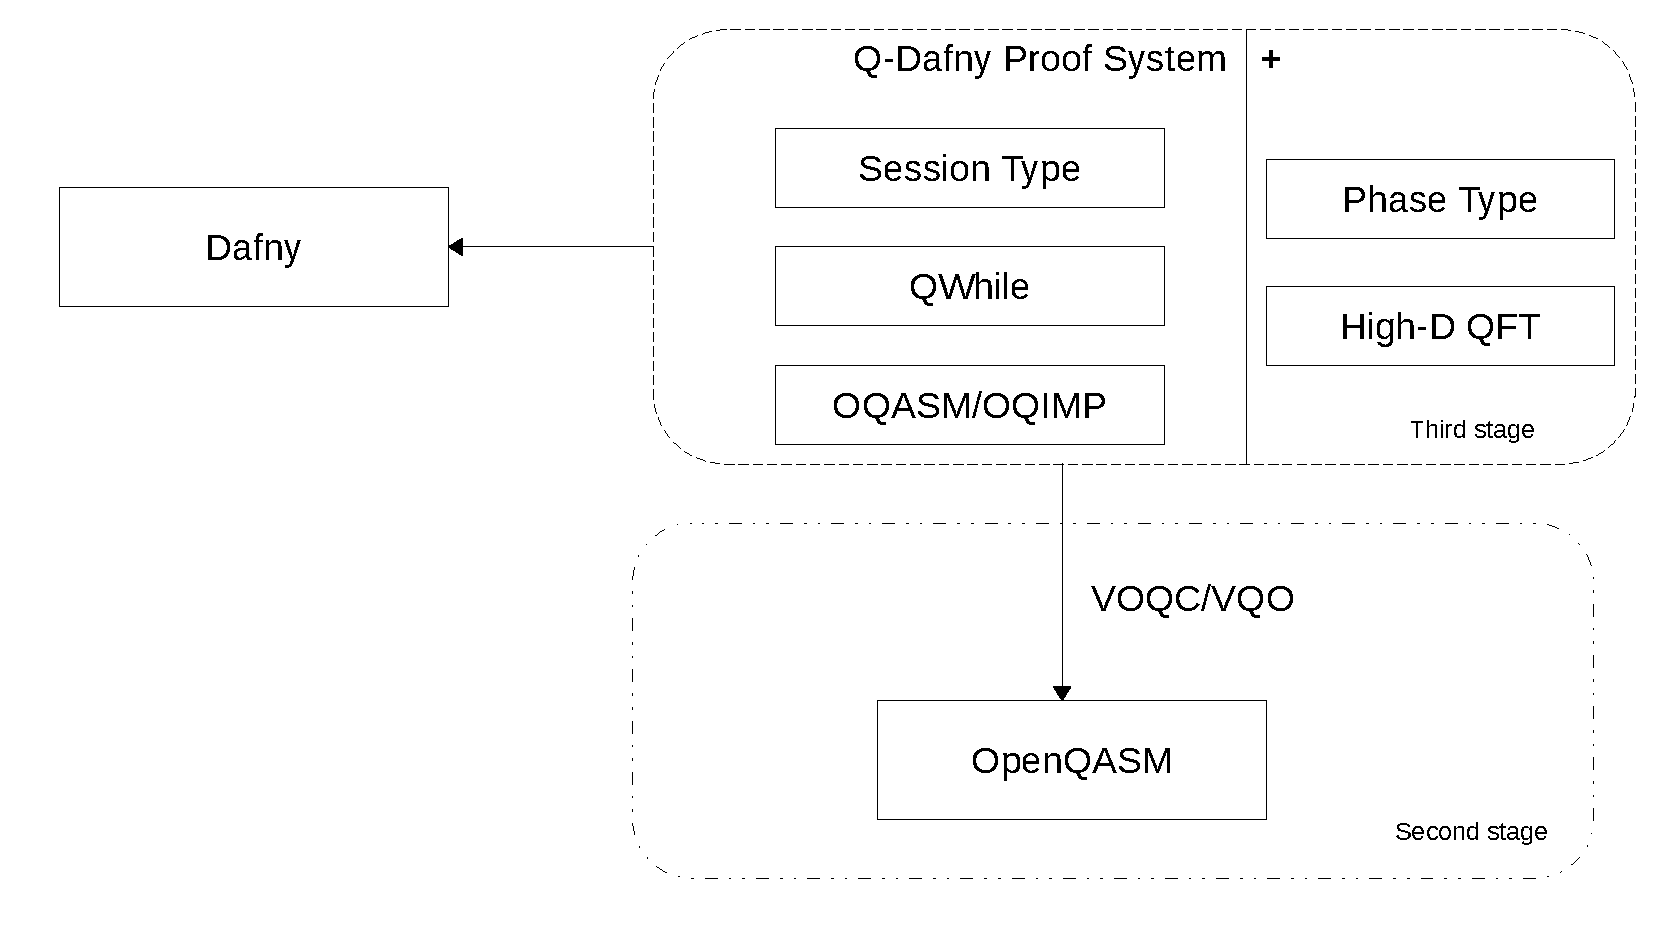
\includegraphics[width=.75\textwidth]{stage}
  \caption{QNP Development Stages and the Key Aspects}
\label{fig:arch}
\end{figure}

On the other hand, there are many classical data state structures that have already had good proof automation theorems,
such as first order array, linked list, and graph theories. 
If we can connect quantum states with these existing classical theories, 
many quantum algorithms can be reasoned by these existing classical proof theories. 
We propose Quantum Natural Proof (QNP), a system to map quantum algorithms 
to classical programs that run on the classical Hoare Logic style proof system, 
and efficiently and automatically certify quantum program properties.
The key observation is that although quantum algorithms running on quantum computers have quantum supremacy,
the structures of many algorithms are simple. 
In addition, the states appearing in these algorithms can be mapped to classical array structures.

\Cref{fig:arch} provides the QNP development plan. 
In the first stage, we develop the Q-Dafny proof system including a quantum language (QWhile) 
that contains operations for writing oracles (\oqasm/\sourcelang),
a type system to record the qubit state forms for easing property proofs, 
as well as a proof system built on top of the classical Hoare Logic array theory.
In addition, Q-Dafny is compiled to Dafny, 
such that a quantum program with its user-defined properties is compiled to Dafny with additional auto-generated Q-Dafny axioms.
The program properties are eventually automatically proved in Dafny with the auto-generated Q-Dafny axioms.
The second stage is to compile programs in QWhile, as a quantum language, to ones in OpenQASM,
such that a verified QWhile program can be run on a quantum computer. 
The third stage upgrades Q-Dafny's type system to track not only quantum state bases but also phases.
Then, a multi-denominational quantum Fourier transformation (High-D QFT) theory can be built on top of the upgraded type system,
so that the Q-Dafny+ proof system is capable of defining advanced quantum algorithms that rely on the High-D QFT theory.
One example is quantum signal processing \cite{Low_2017}.

In this document, we mainly focus on the explanation of the first stage. Here are three key aspects.

\myparagraph{Based on Hoare Logic Array Theory}
We first select the target mapping classical data structure -- arrays, because of two reasons.
First, quantum states can be represented by arrangement of quantum qubits which usually can be thought of as special arrays.
Thus, quantum entanglement of some qubits can be thought as some properties defined on the qubits, 
such that once a qubit is measured, the other qubits consequentially perform some state changes.
Second, classical array structures are the most commonly used data structure 
that has many proved theories and axioms, which does not rely on array sizes, for proof automation;
while other data structure automated proof theories (axioms), such as linked lists, 
finish a property proof by an exclusive proof search on the list of elements in the data structure \cite{DBLP:conf/pldi/Qiu0SM13}.
To represent $n$ qubits as an array in Q-Dafny and verify a property on them, sometimes,
we create a $2^n$ array to capture the entanglement relations among the qubits
and expect the array theory to prove the property symbolically regardless the array size.

\myparagraph{Using a Session Type System to Classify State Forms}
Consequentially, representing quantum states by arrays has its limitations.
Conceptually, state representations in the Q-Dafny proof system
implies the arrange of a set of axioms that facilitate program property proof automation.
Nevertheless, quantum states are high dimensional while arrays are linear.
This fact almost always indicates that the set of axioms might be huge 
and the way of applying the axioms for proof automation is not linear,
so that the proof automation faces major obstacles. 

To overcome these obstacles, we identify three different quantum state representations (\Cref{fig:vqir-state}) in Q-Dafny, 
which are associated with different axioms for proof automation.
Then, the Q-Dafny session type system tracks the transformation of different state 
representations for different \textit{sessions}, collections of qubit array segments that are possibly entangled.
Conceptually, the different state representations guarantee the Q-Dafny proof system can be expressed
in terms of the Hoare Logic array theory.
In compiling Q-Dafny to Dafny,
for proving a local property for a session, we generate and identify different axioms for different state representations,
and we also generate axioms that handle the transformation between state representations.

\begin{figure}[t]
{\small
  \begin{lstlisting}[numbers=left,language=C++,xleftmargin=4 mm]
method Shor ( a : int, N : int, n : int, m : int, x : Q[n], y : Q[n] )
 requires (n > 0)
 requires (1 < a < N)
 requires (N < 2^(n-1))
 requires (N^2 < 2^m <= 2 * N^2)
 requires (gcd(a, N) == 1)
 requires ( type(x) = Tensor n (Nor 0))
 requires ( type(y) = Tensor n (Nor 0))
 ensures (gcd(N, r) == 1)
 ensures (p.pos >= 4 / (PI ^ 2))
{
  x *= H ;
  y *= cl(y+1); //cl can be omitted.
  for (int i = 0; i < n; x[i]; i ++)
    invariant (0 <= i <= n)
    invariant (saturation(x[0..i]))
    invariant (type(y,x[0..i]) = Tensor n (ch (2^i) {k | j baseof x[0..i] && k = (a^j mod N,j)}))
    //psum(k=b,M,p(k),b(k)) = sum_{k=b}^M p(k)*b(k)
    invariant ((y,x[0..i]) == psum(k=0,2^i,1,(a^k mod N,k))) 
  {
    y *= cl(a^(2^i) * y mod N);
  }

 M z := measure(y);//partial measurement, actually measure(y,r) r is the period
 x *= RQFT;
 M p := measure(x); //p.pos and p.base
 var r := post_period(m,p.base) // exists t. 2^m * t / r = p.base
}
  \end{lstlisting}
}
\caption{Shor's Algorithm in Q-Dafny}
\label{fig:shorexample}
\end{figure}


\myparagraph{Enabling Complicated Oracle and Reflection Operations}
The first stage session type system tracks only qubit bases.
As a consequence, the set of quantum algorithms that are efficiently reasonable has the scheme $\texttt{QFT};U;\texttt{QFT}^{-1}$,
where $\texttt{QFT}$ and $\texttt{QFT}^{-1}$ are Hadamard or QFT gates that switch qubits array state forms between normal and superposition, $U$ is an arbitrary combination of QWhile operations that use Hadamard or QFT gates in a manageable manner.
For rich expressiveness, we permit two kinds of managed operations that might involve Hadamard or QFT gates: 
oracle assignments written in \oqasm/\sourcelang and quantum reflection operations (\texttt{amplify} and \texttt{diffuse} in \Cref{fig:vqimp}).
The concept of "management" refers to the fact that there is a type system in \oqasm/\sourcelang to ensure the use of Hadamard or QFT gates do not cause entanglement, as well as the Hadamard or QFT gate usage in quantum reflections has a fixed implementation, such that its semantics is well-known and its property reasoning is captured by Q-Dafny.

Almost all near term quantum algorithms are definable in terms of the above scheme, such as GHZ, Grover's, Shor's, and Childs' Boolean equation algorithms.
To prove properties about advanced quantum algorithms, the session type system needs to track qubit phases, which will complicate its design, and it is the major task of stage 3 in the QNP development.


















%\section{Background}
\label{sec:background}

We begin with some background on quantum computing and quantum algorithms. 

\myparagraph{Quantum States} A quantum state consists of one or more quantum bits (\emph{qubits}). A qubit can be expressed as a two dimensional vector $\begin{psmallmatrix} \alpha \\ \beta \end{psmallmatrix}$ where $\alpha,\beta$ are complex numbers such that $|\alpha|^2 + |\beta|^2 = 1$.  The $\alpha$ and $\beta$ are called \emph{amplitudes}. 
%
We frequently write the qubit vector as $\alpha\ket{0} + \beta\ket{1}$ where $\ket{0} = \begin{psmallmatrix} 1 \\ 0 \end{psmallmatrix}$ and $\ket{1} = \begin{psmallmatrix} 0 \\ 1 \end{psmallmatrix}$ are \emph{computational basis states}. When both $\alpha$ and $\beta$ are non-zero, we can think of the qubit as being ``both 0 and 1 at once,'' a.k.a. a \emph{superposition}. For example, $\frac{1}{\sqrt{2}}(\ket{0} + \ket{1})$ is an equal superposition of $\ket{0}$ and $\ket{1}$. 

We can join multiple qubits together to form a larger quantum state with the \emph{tensor product} ($\otimes$) from linear algebra. For example, the two-qubit state $\ket{0} \otimes \ket{1}$ (also written as $\ket{01}$) corresponds to vector $[~0~1~0~0~]^T$. 
Sometimes a multi-qubit state cannot be expressed as the tensor of individual states; such states are called \emph{entangled}. One example is the state $\frac{1}{\sqrt{2}}(\ket{00} + \ket{11})$, known as a \emph{Bell pair}.
Entangled states lead to exponential blowup: A general $n$-qubit state must be described with a $2^n$-length vector, rather than $n$ vectors of length two. The latter is possible for unentangled states like $\ket{0} \otimes \ket{1}$; \vqir's type system guarantees that qubits remain unentangled.

\begin{figure}[t]
  \centering
\begin{tabular}{c@{$\quad\qquad$}c}
\begin{minipage}[b]{\textwidth}
  \Small
  \Qcircuit @C=0.5em @R=0.5em {
    \lstick{} & \gate{H} & \gate{R_2} & \gate{R_3} & \gate{R_4} & \qw        & \qw            & \qw     &\qw   & \qw &\qw &\qw\\
    \lstick{} & \qw        & \ctrl{-1}       & \qw   &\qw         & \gate{H} & \gate{R_2} & \gate{R_3}      & \qw  & \qw &\qw&\qw\\
    \lstick{} & \qw        & \qw            & \ctrl{-2}       & \qw      &\qw   & \ctrl{-1}      &\qw & \gate{H} & \gate{R_2} &\qw&\qw\\
    \lstick{} & \qw        & \qw           &\qw & \ctrl{-3}       & \qw    &\qw     & \ctrl{-2}      & \qw & \ctrl{-1} & \gate{H} & \qw 
    }
\end{minipage}
&
\begin{minipage}[b]{\textwidth}
  \Small
  \Qcircuit @C=0.5em @R=0.5em {
    \lstick{} & \gate{H} & \gate{R_2} & \gate{R_3} & \qw & \qw        & \qw            & \qw     &\qw   & \qw &\qw &\qw\\
    \lstick{} & \qw        & \ctrl{-1}       & \qw   &\qw         & \gate{H} & \gate{R_2} & \qw      & \qw  & \qw &\qw&\qw\\
    \lstick{} & \qw        & \qw            & \ctrl{-2}       & \qw      &\qw   & \ctrl{-1}      &\qw & \gate{H} & \qw &\qw&\qw\\
    \lstick{} & \qw        & \qw           &\qw & \qw       & \qw    &\qw     & \qw      & \qw & \qw & \gate{H} & \qw 
    }
\end{minipage}
\end{tabular}
\caption{Example quantum circuits: QFT over 4 qubits (left) and approximate QFT with 3 qubit precision (right). $R_m$ is a $z$-axis rotation by $2\pi / 2^m$.}
\label{fig:background-circuit-example}
\end{figure}

\myparagraph{Quantum Circuits} 
Quantum programs are commonly expressed as \emph{circuits}, like those shown in \Cref{fig:background-circuit-example}. In these circuits, each horizontal wire represents a qubit, and boxes on these wires indicate quantum operations, or \emph{gates}. Gates may be \emph{controlled} by a particular qubit, as indicated by a filled circle and connecting vertical line. The circuits in  \Cref{fig:background-circuit-example} use four qubits and apply 10 (left) or 7 (right) gates: four \emph{Hadamard} ($H$) gates and several controlled $z$-axis rotation (``phase'') gates.
%
When programming, circuits are often built by meta-programs embedded in a host language, e.g., Python (for Qiskit~\cite{Qiskit}, Cirq~\cite{cirq}, PyQuil~\cite{PyQuil}, and others), Haskell (for Quipper~\cite{Green2013}), or Coq (for \sqir and our work).

\myparagraph{Quantum Fourier Transform}
The quantum Fourier transform (QFT) is the quantum analogue of the discrete Fourier transform.
It is used in many quantum algorithms, including the phase estimation portion of Shor's factoring algorithm~\cite{shors}.
The standard implementation of a QFT circuit (for 4 qubits) is shown on the left of \Cref{fig:background-circuit-example}; an \emph{approximate QFT} (AQFT) circuit can be constructed by removing select controlled phase gates~\cite{ApproximateQFT,appox-qft2,appox-qft1}.
This produces a cheaper circuit that implements an operation mathematically similar to the QFT.\@
The AQFT circuit we use in \name (for 4 qubits) is shown on the right of \Cref{fig:background-circuit-example}. 
When it is appropriate to use AQFT in place of QFT is an open research problem, and one that is partially addressed by our work on \oqasm, which allows efficient testing of the effect of AQFT inside of oracles.

\myparagraph{Computational and QFT Bases}
The computational basis is just one possible basis for the underlying vector space.
Another basis is the \emph{Hadamard basis},  written as a tensor product of $\{\ket{+}, \ket{-}\}$, obtained by applying a \emph{Hadamard transform} to elements of the computational basis, where $\ket{+}=\frac{1}{\sqrt{2}}(\ket{0}+\ket{1})$ and  $\ket{-}=\frac{1}{\sqrt{2}}(\ket{0}-\ket{1})$.
A third useful basis is the \emph{Fourier (or QFT) basis}, obtained by applying a \emph{quantum Fourier transform} (QFT) to elements of the computational basis.

% Analogous to the position and momentum representations in Schrodinger's picture of quantum mechanics, there are also two commonly used special bases in the finitely dimensional Hilbert space studied in quantum information. The computational basis refers to classical bit strings written as the tensor product of $\{\ket{0}, \ket{1}\}$, while the dual basis, or the Fourier basis, is obtained by applying \emph{quantum Fourier transformation} (QFT) on the computational basis. The computational space refers to the space spanned by the computational basis, and similarly to the dual space, although the computational and dual spaces are isomorphic to each other.  As shown by~\citet{qft-adder}, arithmetic on the computational basis can sometimes be more efficiently carried in the dual basis, which leads to the use of quantum operations in optimizing circuits with classical functionalities. 


\ignore{
Applying a gate to a state \emph{evolves} the state. The semantics of doing so is expressed by multiplying the state vector by the gate's corresponding matrix representation; single-qubit gates are 2-by-2 matrices, and two-qubit gates are 4-by-4 matrices. A gate's matrix must be \emph{unitary}, ensuring that it preserves the unitarity invariant of quantum states' amplitudes. An entire circuit can be expressed as a matrix by composing its constituent gates.
}

\myparagraph{Measurement} A special, non-unitary \emph{measurement} operation extracts classical information from a quantum state, typically when a computation completes. Measurement collapses the state to a basis states with a probability related to the state's amplitudes. For example, measuring $\frac{1}{\sqrt{2}}(\ket{0} + \ket{1})$ in the computational basis will collapse the state to $\ket{0}$ with probability $\frac{1}{2}$ and likewise for $\ket{1}$, returning classical value 0 or 1, respectively. In all the programs discussed in this paper, we leave the final measurement operation implicit.

\myparagraph{Quantum Algorithms and Oracles}

Quantum algorithms manipulate input information encoded in ``oracles,'' which are callable black box circuits. For example, Grover's algorithm for unstructured quantum search \cite{grover1996,grover1997} is a general approach for searching a quantum ``database,''  which is encoded in an oracle for a function $f : \{0, 1\}^n \to \{0, 1\}$. Grover's finds an element $x \in \{0, 1\}^n$ such that $f(x) = 1$ using $O(2^{n/2})$ queries, a quadratic speedup over the best possible classical algorithm, which requires $\Omega(2^n)$ queries.
% Another famous example is Shor's prime factoring algorithm \cite{shors}, which uses an oracle that performs modular exponentiation. Oracles can dominate the size of the overall quantum program: In the implementation of Shor's, more than 90\% of gates are in the oracle~\cite{Gidney2021howtofactorbit}.
An oracle can be constructed for an arbitrary function $f$ simply by constructing a reversible classical logic circuit implementing $f$ and then replacing classical logic gates with corresponding quantum gates, e.g.,
\texttt{X} for ``not,'' \texttt{CNOT} for ``xor,'' and \texttt{CCNOT} (aka \emph{Toffoli}) for ``and.'' However, this approach does not always produce the most efficient circuits; for example, quantum circuits for arithmetic can be made more space-efficient using the quantum Fourier transform \cite{2000quant}.

%\paragraph{Uncomputation}

% When quantum algorithms are applied to solve classical problems, the oracle $f$ is inherently classical. 
% Programming oracles requires transforming a (potentially large) classical expression into a reversible classical circuit, and then into a quantum circuit.
Transforming an irreversible computation into a quantum circuit often requires introducing ancillary qubits, or \emph{ancillae}, to store intermediate information \cite[Chapter 3.2]{mike-and-ike}.
Oracle algorithms typically assume that the oracle circuit is reversible, so any data in ancillae must be \emph{uncomputed} by inverting the circuit that produced it.
Failing to uncompute this information leaves it entangled with the rest of the state, potentially leading to incorrect program behavior.
To make this uncomputation more efficient and less error-prone, recent programming languages such as Silq \cite{sliqlanguage} have developed notions of \emph{implicit} uncomputation.
We have similar motivations in developing \name: we aim to make it easier for programmers to write efficient quantum oracles, and to assure, through verification and randomized testing, that they are correct.



% Writing a quantum algorithm now, with SQIR (but likewise with Quipper, Pyquil, Circ, etc.). Example: Shor’s
% Write quantum parts (QPE) 
% Classical parts via library functions in meta-language (Modular multiplier)
% Refer to particular quipper functions, e.g., for adding, subtraction, etc.
% https://www.mathstat.dal.ca/~selinger/quipper/doc/Quipper-Libraries-QFTAdd.html qft_add_in_place :: QDInt -> QDInt -> Circ (QDInt, QDInt), Add one QDInt onto a second, in place; i.e. (x,y) ↦ (x,x+y). Arguments are assumed to be of equal size. This implementation follows the implementation in Thomas G. Draper's paper "Addition on a Quantum Computer" which doesn't require the use of any ancilla qubits through a clever use of the quantum Fourier transform.
% Mention Q# too
% https://github.com/microsoft/QuantumLibraries/tree/main/Numerics/src
% Maybe Scaffold:
% Write oracles via “RKQC intrinsic” functions (see sec 4.1 of https://iopscience.iop.org/article/10.1088/2058-9565/ab8c2c/pdf). The intrinsics they talk about here are super simple (swap two registers or add two registers together)
% Quipper: Write in Haskell, build_circuit, is better
% Problems to solve: Efficient compilation, verification of that compilation
% Verification: Prior work with ReverC, but only classical gates

%\input{overview}
\section{QWhile: A High-level Quantum Language}
\label{sec:vqir}

We introduce the language syntax and type system for QWhile and introduce the Q-Dafny Proof system.
As a running example, we specify Shor's algorithm and its proof in Q-Dafny in \Cref{fig:shorexample}.
The Q-Dafny to Dafny compiler is under construction, but the compiled version of the Shor's algorithm proof has been finalized
and can be found at \url{https://github.com/inQWIRE/VQO/blob/naturalproof/Q-Dafny/examples/Shor-compiled.dfy}.


\subsection{Syntax}
\sloppy
QWhile is a high-level language for describing quantum programs,
which permits quantum control and for-loop statements.
\Cref{fig:vqimp} introduces the QWhile syntax. 

\begin{figure}[t]
{
  \small
  \[\begin{array}{llcl} 
      \text{Nat. Num} & m, n & \in & \mathbb{N}       \\
      \text{Real} & r & \in & \mathbb{R}\\
      \text{Variable} & x,y \\
      \text{\cmode-Mode Value} & n\\
      \text{\mmode-Mode Value} & (r,n)\\
      \text{\oqasm Expr} & \mu\\
      \text{Session} & \zeta & ::= & \overline{(x,n,m)} \\
      \text{Type Predicate} & T & ::= & x:\tau  \mid x:\{\zeta:\tau\} \mid ...\\
      \text{State Predicate} & P,Q & ::= & x=n\mid x=(r,n)  \mid \zeta=\rho \mid ...\\
      \text{Mode} & g & ::= & \cmode  \mid \mmode\\
      \text{Mode Check Result} & q & ::= & g  \mid \zeta\\
      \text{Factor} & l & ::= & x \mid x[a] \\
      \text{Arith Expr} & p,a & ::= & l \mid a + a \mid a * a \mid ... \\
      \text{Bool Expr} & b & ::= & x[a] \mid (a = a) @ x[a] \mid (a < a) @ x[a] \mid \neg b  ... \\
      \text{Gate Expr} & op & ::= & \texttt{H} \mid \iqft[\lbrack -1 \rbrack]{}{} \\
      \text{C/M Moded Expr}& e & ::= & a \mid \smea{y}  \\
      \text{Statement} & s & ::= & \sskip \mid \sexp{x}{e}{s} \mid  \ssassign{l}{}{op} \mid \ssassign{\overline{l}}{}{a(\mu)} 
                                 \\ & & \mid & \sseq{s}{s} \mid \sifq{b}{s} \mid
                                     \sqwhile{\sinit{i}{a_1}}{i<a_2}{b(i)}{f(i)}{T(i)}{P(i)}{s}
                     \\&&\mid & \samplify{\ssassign{x}{}{a}}
                      \mid \sdistr{l}
    \end{array}
  \]
}
{\footnotesize
\[
\begin{array}{l}
\rho \text{: Quantum States see \Cref{fig:vqir-state}}
\end{array}
\]
}
  \caption{Core QWhile Syntax, \oqasm Syntax is in \Cref{fig:vqir}}
  \label{fig:vqimp}
\end{figure}

\begin{figure}[t]
  \small
  \[\hspace*{-0.5em}
\begin{array}{l>{$} p{1.2cm} <{$} c l}
      \text{Bit} & d & ::= & 0 \mid 1 \\
      \text{BitString} & \overline{d} & ::= & \mathbb{N} \to d \\
      \text{BitString Indexed Set} & \beta & ::= & \{\overline{d} \} \mid \infty \\
      \text{Phase Type} & w & ::= & \bigcirc \mid \infty \\
      \text{Type Element} & t & ::= & \tnor{\overline{d}} \mid \thad{w} \mid \tch{n}{\beta}\\
      \text{Type} & \tau & ::= & \ttype{n}{t}\\
      \text{Phase} & \alpha(n) & := & e^{2\pi i \frac{1}{n}} \\
      \text{Amplitude} & \theta & := & r \\
      \text{Phi State} & \qket{n} & := & \frac{1}{\sqrt{2}} (\ket{0}+\alpha(n)\ket{1}) \\
      \text{Quantum State} & \rho & ::= & \alpha\ket{\overline{d}}\mid \Motimes_{k=0}^{m}\ket{\Phi(n_k)}
                                         \mid \sum_{k=0}^{m}\theta_k\ket{\overline{d_k}}
    \end{array}
  \]
  \caption{QWhile Sessions and Types and Quantum States}
  \label{fig:vqir-state}
\end{figure}


\begin{figure}[t]
{\Small
  \begin{mathpar}
    \inferrule[ ]{ }{\Omega \vdash x : \Omega(x)}

    \inferrule[ ]{\Omega(x)=(x,0,\Sigma(x)) }{\Omega \vdash x[n] : [(x,n,n+1)]}

    \inferrule[ ]{ \Omega \vdash a_1 : q_1 \\ \Omega \vdash a_2 : q_2 }{\Omega \vdash a_1 + a_2 : q_1 \sqcup q_2}   

    \inferrule[ ]{ \Omega \vdash a_1 : q_1 \\ \Omega \vdash a_2 : q_2 }{\Omega \vdash a_1 * a_2 : q_1 \sqcup q_2}   
 

    \inferrule[ ]{ \Omega \vdash a_1 : q_1 \\ \Omega \vdash a_2 : q_2 \Omega \vdash a_3 : q_3  }{\Omega \vdash (a_1 = a_2)@x[n] : q_1 \sqcup q_2\sqcup q_3}   

    \inferrule[ ]{ \Omega \vdash a_1 : q_1 \\ \Omega \vdash a_2 : q_2 \Omega \vdash a_3 : q_3  }{\Omega \vdash (a_1 < a_2)@x[n] : q_1 \sqcup q_2\sqcup q_3}

    \inferrule[ ]{ \Omega \vdash b : q}{\Omega \vdash \neg b : q}  

    \inferrule[ ]{ \Omega \vdash e : \zeta_2 \sqcup \zeta_1 }{\Omega \vdash e : \zeta_1 \sqcup \zeta_2}   

  \end{mathpar}
}
{\footnotesize
\[
\begin{array}{l}
\zeta_1 \sqcup \zeta_2 = \zeta_1 \uplus \zeta_2
\zeta \sqcup g = \zeta
\qquad 
g \sqcup \zeta = \zeta
\qquad
\cmode \sqcup \cmode = \cmode
\qquad
\mmode \sqcup \cmode = \mmode
\qquad
\cmode \sqcup \mmode = \mmode
\qquad
\cmode \le \mmode \le \zeta
\\[0.2em]
\bot \uplus l = l
\qquad 
l \uplus \bot = l

\qquad

[(x,v_1,v_2)] \uplus [(y,v_3,v_4)] = [(x,v_1,v_2), (y,v_3,v_4)]

\\

[v_2,v_2] \cap [v_3,v_4] \neq \emptyset \Rightarrow [(x,v_1,v_2)] \uplus [(x,v_3,v_4)] = [(x,\texttt{min}(v_1,v_3),\texttt{max}(v_2,v_4))]

\end{array}
\]
}
  \caption{Arith, Bool, Gate Mode Checking}
  \label{fig:exp-well-typed}
\end{figure}

A QWhile program consists of a sequence of C-like statements $s$.
Values and variables (ranged by $x$ and $y$) in a statement
are classified as three different categories: compilation time classical values, 
classical values generated from quantum measurement, and quantum state registers.
We use variable \textit{modes} to classify the first two kinds as \cmode and \mmode modes.
We represent \cmode-mode values as natural numbers, while $M$-mode values are represented as pairs of reals and natural numbers.
The reals represent the conceptual occurrence probability of the result measurement,
and the natural numbers are the measurement results.
Any further arithmetic operations on $M$-mode values are applied on the measurement results,
such as $(r,n_1)+n_2=(r,n_1+n_2)$.

Quantum registers refer to quantum qubit arrays in QWhile.
They are always associated with disjoint sets of qubit array fragments, named \textit{sessions}.
We represent a qubit array fragment as $(x,n,m)$, where $x$ is a variable representing a qubit array, $n$ is the start position in $x$ for the array fragment and $m$ is the exclusive ending point.
In \Cref{fig:shorexample}, an example array fragment for \code{x} is \code{x[0..i]}.
\code{y} is an abbreviation of array fragment \code{y[0..n]} where \code{n} is the ending point of array \code{y}.
\code{(y,x[0..i])} is a session containing two array fragments.
It is worth noting that the ordering of fragments in a session only 
serves for recording the qubit positions in a quantum register.
The swapping of fragment ordering does not affect the register state.
In Q-Dafny, the fragment ordering might affect the property proof automation.
In \Cref{fig:shorexample}, we fix fragment order as \code{(y,x[0..i])}
to enhance the Shor's algorithm proof automation. 

We use $x[a]$ to represent the $a$-th position qubit in $x$.
It is worth noting that the variable $x$ in $x[a]$ must represent quantum registers. 
We name a variable $x$ or an array index $x[a]$ as a factor.
In a QWhile program, \cmode and \mmode mode variables act like stack variables
and they must be bounded by variables introduced by \texttt{let} statements;
while quantum registers represent arrays in a "quantum heap" and are bounded by $\Sigma$.

The statements $s$ in the first row in \Cref{fig:vqimp} are \sskip (SKIP) and assignment operations.
Classic assignment (\sexp{x}{e}{s}) evaluates $e$ and assigns the value to \cmode or \mmode mode variable $x$ that is used in $s$.
Expressions $e$ can be an arithmetic or a measurement operation.
$\sexp{x}{\smea{y}}{...}$ assigns the measurement result of qubit array $y$ to $x$.
$\ssassign{l}{}{op}$ and $\ssassign{\overline{l}}{}{a(\mu)}$ are quantum assignments.
The former applies a simple quantum gate ($\texttt{H}$ or $\texttt{QFT}$)
to a single qubit ($x[a]$) or a qubit array ($x$) \footnote{$\texttt{QFT}$ gate must apply to a variable $x$}.
$\ssassign{\overline{l}}{}{a(\mu)}$ is a generalized quantum assignment that implements quantum oracle circuits $a$ and applies an \oqasm/\sourcelang operation on a list of qubit array $\overline{l}$.
We assume all arithmetic ($a$) and Boolean ($b$) expressions are reversible.
For example, the operation $(a_1 < a_2) @ x[a]$ compares $a_1$ and $a_2$ and stores the value in $x[a]$.
$\mu$ is the circuit implementation of the expression $a$ in \oqasm, whose syntax is given in \Cref{sec:vqir}.
One can utilize \oqasm expressions ($\mu$) to implement singleton $\texttt{X}$ and $\irz[\lbrack -1 \rbrack]{n}{}$ gates,
thus, the QWhile syntax is universal with respect to quantum gates.
In addition, \sourcelang is a C-like reversible arithmetic language built on \oqasm.
The reversible expression $a$ in \Cref{fig:vqimp} is based on \sourcelang operations.
For simplicity, we write $\ssassign{\overline{l}}{}{a}$ in examples here to
mean that it applies a \sourcelang circuit that computes $a$ to $\overline{l}$.

The second row of statements in \Cref{fig:vqimp} are control-flow operations.
$\sseq{s_1}{s_2}$ is a sequential operation.
$\sifq{b}{s}$ is a conditional and $b$ might contain quantum factors.
Every quantum factor $l$ appearing in $b$ must not appear in $s$.
In QWhile, we define a \texttt{well\_formed} predicate to check such property.
$\sqwhile{\sinit{i}{a_1}}{i<a_2}{b(i)}{f(i)}{T(i)}{P(i)}{s}$ is a possibly quantum for-loop depending on if the Boolean guard $b(i)$ ($b(i)$ is a Boolean expression that contains variable $i$) contains quantum factors (also needing to be \texttt{well\_formed}).
A classical variable $i$ is introduced and it is initialized as the lower bound $a_1$, increments in each loop step by the monotonic increment function $f(i)$, and ends at the upper bound $a_2$.
$T(i)$ is the type predicate (type predicate syntax in \cref{fig:vqimp}) where for $i$-th loop step,
$T(i)$ is true in the beginning and $T(f(i))$ is maintained after the execution.
Similarly, $P(i)$ is the loop-invariant (state predicate in \cref{fig:vqimp}) for the for-loop structure, where for $i$-th loop step,
$P(i)$ is true in the beginning and $P(f(i))$ is maintained after the execution. 

The last row contains quantum reflection operations,
which are used to adjust the occurrence probability of
some quantum states in a quantum qubit array.
For example, in Grover's search algorithm \cite{grover1996},
the Grover's diffusion operation is a quantum reflection
that increases the occurrence probability of a target quantum state in a qubit array being in superposition.
We identify two kinds of quantum reflections that previous works tent to combine together.
The first one is an amplifier ($\samplify{\ssassign{x}{}{a}}$)
that amplifies the occurrence probability of the target state,
which is represented by a classical value $a$,
in a quantum qubit array $x$.
The second one is a diffusion operator ($\sdistr{x}$)
that diffuses the state of a qubit array $x$ to a superposition of 
all possible bases in $x$ with possibly different amplitudes \footnote{The possible bases do not depend on $x$'s state, and it is only related to the qubit size of $x$; i.e., if $x$ is a two qubit array, then the operation reflects the superposition of all possible two qubit states as: $\frac{1}{2}(\ket{00}+\ket{01}+\ket{10}+\ket{11})$.  }.
For example, applying the diffusion operator on a two-qubit array $x$ having state $\ket{00}$
results in a superposition of $-\frac{1}{2}\ket{00}+\frac{1}{2}\ket{01}+\frac{1}{2}\ket{10}+\frac{1}{2}\ket{11}$.
In general, if an $n$-qubit array $x$ has the state $\sum_{j=0}\alpha_j\ket{x_j}$,
the result of applying a diffusion operator is $\frac{1}{2^{n}}(2\sum_{i=0}^{2^n}(\sum_{j=0}\alpha_j)\ket{i} - \sum_{j=0}\alpha_j\ket{x_j})$.

\subsection{Type Checking: A Quantum Session Type System}\label{sec:typesystem}

The QWhile type system can be viewed as a mapping from lists of factors ($x$ or $x[n]$) to QWhile types in \Cref{fig:vqir-state}.
Generally, factors represent a range of locations in a "quantum heap".
Variable $x$ can be viewed as a range $(x,0,\Sigma(x))$, meaning the heap range starting at $x$ and ending at $x+n$.
Index $x[n]$ can be viewed as a range $(x,n,n+1)$.
Thus, a list of \textbf{quantum} factors is essentially a list of disjoint fragments, which it is called a \textit{session}.

A type is written as $\ttype{n}{t}$, where $n$ refers to the total number of qubits in a session,
and $t$ describes the qubit state form. 
A session being type $\ttype{n}{\tnor{\overline{d}}}$
means that every qubit is in normal basis (either $\ket{0}$ or $\ket{1}$),
and $\overline{d}$ describes basis states for the qubits.
The type corresponds to a single qubit basis state $\alpha(n)\ket{\overline{d}}$,
where the global phase $\alpha(n)$ has the form $e^{2 \pi i \frac{1}{n}}$ and $\overline{d}$ is a list of bit values.
Global phases for \texttt{Nor} type are usually ignored in many semantic definitions.
In QWhile, we record it because in quantum conditionals, such global phases might be turned to local phases.

$\ttype{n}{\thad{w}}$ means that every qubit in the session has the state: $(\alpha_1\ket{0} + \alpha_2\ket{1})$;
the qubits are in superposition but they are not entangled.
$\bigcirc$ represents the state is a uniform superposition,
while $\infty$ means the phase amplitude for each qubit is unknown.
If a session has such type, it then has the value form $\Motimes_{k=0}^{m}\ket{\Phi(n_k)}$,
where $\ket{\Phi(n_k)}=\frac{1}{\sqrt{2}}(\ket{0}+\alpha(n_k)\ket{1})$.

All qubits in a session that has type $\ttype{n}{\tch{m}{\beta}}$ are supposedly entangled (eventual entanglement below).
$m$ refers to the number of possible different entangled states in the session,
and the bitstring indexed set $\beta$ describes each of these states, while every element in $\beta$ is indexed by $i\in [0,m)$.
$\beta$ can also be $\infty$ meaning that the entanglement structure is unknown.
For example, in quantum phase estimation, after applying the $\texttt{QFT}^{-1}$ operation, the state has type $\ttype{n}{\tch{m}{\infty}}$. In such case, the only quantum operation to apply is a measurement.
If a session has type $\ttype{n}{\tch{m}{\beta}}$ and the entanglement is a uniform superposition,
we can describe its state as $\sum_{i=0}^{m}{\frac{1}{\sqrt{m}}\beta(i)}$, and the length of bitstring $\beta(i)$ is $n$.
For example, in a $n$-length GHZ application, the final state is: $\ket{0}^{\otimes n}+\ket{1}^{\otimes n}$. 
Thus, its type is $\ttype{n}{\tch{2}{\{\overline{0}^n,\overline{1}^n\}}}$, where $\overline{d}^n$ is a $n$-bit string having bit $d$.

The type $\ttype{n}{\tch{m}{\beta}}$ corresponds to the value form $\sum_{k=0}^{m}\theta_k\ket{\overline{d_k}}$.
$\theta_k$ is an amplitude real number, and $\overline{d_k}$ is the basis.
Basically, $\sum_{k=0}^{m}\theta_k\ket{\overline{d_k}}$ represents a size $m$ array of basis states
that are pairs of $\theta_k$ and $\overline{d_k}$. For a session $\zeta$ of type $\texttt{CH}$,
one can use $\zeta[i]$ to access the $i$-th basis state in the above summation, and the length is $m$.
In the Q-Dafny implementation section, we show how we can represent $\theta_k$ for effective automatic theorem proving.

The QWhile type system has the type judgment: $\Omega,\itau\vdash_g s : \zeta\triangleright \tau$, where $g$ is the context mode, mode environment $\Omega$ maps variables to modes or sessions ($q$ in \Cref{fig:vqimp}), type environment $\itau$ maps a session to its type, $s$ is the statement being typed, $\zeta$ is the session of $s$, and $\tau$ is $\zeta$'s type. 
The QWhile type system in \Cref{fig:exp-sessiontype} has several tasks. First, it enforces context mode restrictions.
Context mode $g$ is either \cmode or \mmode.
$Q$ represents the current expression lives inside a quantum conditional or loop, while \cmode refers to other cases.
In a $Q$ context, one cannot perform $M$-mode operations, i.e., no measurement is allowed.
There are other well-formedness enforcement. For example,
the session of the Boolean guard $b$ in a conditional/loop is disjoint with the session in the conditional/loop body,
i.e., qubits used in a Boolean guard cannot appear in its conditional/loop body.

Second, the type system enforces mode checking for variables and expressions in \Cref{fig:exp-well-typed}.
In QWhile, \cmode-mode variables are evaluated to values during type checking.
In a \texttt{let} statement (\Cref{fig:exp-sessiontype}),
\cmode-mode expression is evaluated to a value $n$, and the variable $x$ is replaced by $n$ in $s$.
The expression mode checking (\Cref{fig:exp-well-typed}) has the judgment: $\Omega \vdash (a\mid b) : q$. It takes a mode environment $\Omega$, and an expression ($a$, $b$), and judges if the expression has the mode $g$ if it contains only classical values, or a quantum session $\zeta$ if it contains some quantum values. 
All the supposedly \cmode-mode locations in an expression are assumed
to be evaluated to values in the type checking step,
such as the index value $x[n]$ in difference expressions in \Cref{fig:exp-well-typed}.
It is worth noting that the session computation ($\uplus$)
is also commutative as the last rule in \Cref{fig:exp-well-typed}.

Third, by generating the session of an expression, the QWhile type system assigns a type $\tau$ for the session indicating its state format, which will be discussed shortly below. Recall that a session is a list of quantum qubit fragments.
In quantum computation, qubits can entangled with each other.
We utilize type $\tau$ (\Cref{fig:vqir-state}) to state entanglement properties appearing in a group of qubits.
It is worth noting that the entanglement property refers to \textit{eventual entanglement}, .i.e. a group of qubits that are eventually entangled. Entanglement classification is tough and might not be necessary. In most near term quantum algorithms, such as Shor's algorithm \cite{shors} and Childs' Boolean equation algorithm (BEA) \cite{ChildsNAND}, programmers care about if qubits eventually become entangled during a quantum loop execution. This is why the normal basis type ($\ttype{n}{\tnor{\overline{d}}}$) can also be a subtype of a entanglement type ($\ttype{n}{\tch{1}{\{\overline{d}\}}}$) in our system (\Cref{fig:exp-subtyping}).

\myparagraph{Entanglement Types}
We first investigate the relationship between the types and entanglement states.
It is well-known that every single quantum gate application
does not create entanglement ($\texttt{X}$, $\texttt{H}$, and $\texttt{RZ}$).
It is enough to classify entanglement effects through a control gate application, i.e., 
$\sifq{x[i]}{e(y)}$, where the control node is $x[i]$ and $e$ is an operation applying on $y$.

A qubit can be described as $\alpha_1\ket{b_1}+\alpha_2\ket{b_2}$,
where $\alpha_1$/$\alpha_2$ are phase amplitudes, and $b_1$/$b_2$ are bases.
For simplicity, we assume that
when we applying a quantum operation on a qubit array $y$, we either solely change the qubit amplitudes or bases.
We identify the former one as $\mathpzc{R}$ kind, referring to its similarity of applying an \texttt{RZ} gate;
and the latter as $\mathpzc{X}$ kind, referring to its similarity of applying an \texttt{X} gate.
The entanglement situation between $x[i]$ and $y$ after applying a control statement $\sifq{x[i]}{e(y)}$ is described in \Cref{fig:control-entanglement}.

\begin{figure*}[t]
{\footnotesize
\begin{tabular}{|c|c|c|c|c|c|c|c|c|c|}
\hline                           
&  Case 1 & Case 2 & Case 3 & Case 4 & Case 5 & Case 6 & Case 7 & Case 8 & Case 9 \\
\hline
$x[i]$ & \texttt{Nor} & \texttt{Had} & \texttt{Had} & \texttt{Had} & \texttt{Had} & \texttt{Had} & \texttt{Had} & \texttt{CH} & \texttt{CH} \\
$y$  & any & \texttt{Nor} & \texttt{Nor} & \texttt{Had} & \texttt{Had} & \texttt{CH} & \texttt{CH} & \texttt{CH} & \texttt{CH}   \\\hline
$y$'s operation type  & any & $\mathpzc{X}$ & $\mathpzc{R}$ & $\mathpzc{X}$ & $\mathpzc{R}$ & $\mathpzc{X}$ & $\mathpzc{R}$ &  $\mathpzc{X}$ & $\mathpzc{R}$ \\\hline
Output Type Entangled?  & N & Y & N & N & Y & Y & Y & Y & Y  \\
\hline                           
\end{tabular}
  \caption{Control Gate Entanglement Situation}
  \label{fig:control-entanglement}
}
\end{figure*}

If $x[i]$ has input type \texttt{Nor}, the control operation acts as a classical conditional, i.e., no entanglement is possible.
In most quantum algorithms, $x[i]$ will be in superposition (type \texttt{Had}) to enable entanglement creation.
When $y$ has type $\texttt{Nor}$, if $y$'s operation is of $\mathpzc{X}$ kind, an entanglement between $x[i]$ and $y$ is created, such as the GHZ algorithm; 
if the operation is of $\mathpzc{R}$ kind, there is not entanglement after the control application, such as the Quantum Phase Estimation (QPE) algorithm.

When $x[i]$ and $y$ are both of type \texttt{Had}, if we apply an $\mathpzc{X}$ kind operation on $y$,
it does not create entanglement. An example application is the phase kickback pattern.
If we apply a $\mathpzc{R}$ operation on $y$, this does create entanglement.
This kind of operations appears in state preparations, such as preparing a register $x$ to have state $\sum_{t=0}^N i^{-t}\ket{t}$ in Childs' Boolean equation algorithm \cite{ChildsNAND}. 
The main goal for preparing such state is not to entanglement qubits, but to prepare a state with phases related to its bases.

\begin{figure}[t]
{\small
$
\begin{array}{l}
\ttype{n}{\tnor{\overline{d}}} \sqsubseteq \ttype{n}{\tch{1}{\{\overline{d}\}}}
\qquad 
\ttype{n}{\tch{2^n}{\beta}} \sqsubseteq \ttype{n}{\tch{2^n}{\infty}}
\qquad 
\ttype{n}{\thad{\bigcirc}} \sqsubseteq \ttype{n}{\tch{2^n}{\tpower{n}}}
\end{array}
$
}
  \caption{Session Type Subtyping}
  \label{fig:exp-subtyping}
\end{figure}

The case when $x[i]$ and $y$ has type \texttt{Had} and \texttt{CH}, respectively,
happens in the middle of executing a quantum loop, such as in the Shor's algorithm and BEA.
Applying both $\mathpzc{X}$ and $\mathpzc{R}$ kind operations result in entanglement.
In this narrative, algorithm designers intend to
merge an additional qubit $x[i]$ into an existing entanglement session $y$.
$x[i]$ is commonly in uniform superposition,
but there can be some additional local phases attached with some bases,
which we named this situation as saturation, i.e.,
In an entanglement session written as $\sum_{i=0}^n \ket{x_l,y,x_r}$,
for any fixing $x_l$ and $x_r$ bases, if $y$ covers all possible bases,
we then say that the part $y$ in the entanglement is in saturation.
This concept is important for generating auto-proof, which will be discussed in \Cref{sec:logical}.

\begin{figure}[t]
{
{\Small
  \begin{mathpar}

    \inferrule[TA-NOR]{ \Omega \vdash \overline{l}:\zeta
                  \\ \llbracket a \rrbracket\ket{\overline{d}}=\alpha\ket{\overline{d'}}}{\Omega,\itau[\zeta \mapsto \ttype{n}{\tnor{\overline{d}}}] \vdash_g \ssassign{\overline{l}}{}{a} : \zeta \triangleright_g \ttype{n}{\tnor{\overline{d'}}} }


    \inferrule[TA-HAD]{ \Omega \vdash \overline{l}:\zeta\\ \zeta \subseteq \zeta'
                  \\ (\forall \overline{d}\;.\;\llbracket a \rrbracket\ket{\overline{d}}=\ket{\overline{d'}}) \\ }{\Omega,\itau[\zeta'\mapsto \ttype{n}{\thad{\bigcirc}}] \vdash_g \ssassign{\overline{l}}{}{a} : \zeta' \triangleright \ttype{n}{\thad{\bigcirc}}}

    \inferrule[TEXP]{\Omega[x\mapsto \cmode],\itau\vdash_g s[v/x] :\zeta \triangleright \tau}{\Omega,\itau \vdash_g \sexp{x}{v}{s} :\zeta\triangleright \tau }

    \inferrule[TMEA]{ \Omega \vdash y:\zeta \\ n'=\size{\zeta'}
     \\ m' = \texttt{size}(\{\overline{c'}|\overline{c}\cdot\overline{c'}\in\beta\cdot\beta'\wedge \overline{c}=\texttt{val}(x)\})
\\\\
           \Omega[x\mapsto \mmode],\itau[\zeta' \mapsto \ttype{n'}{\tch{m'}{\{\overline{c'}|\overline{c}\cdot\overline{c'}\in\beta\cdot\beta'\wedge \overline{c}=\texttt{val}(x)\}}}]\vdash_{\cmode} s : \zeta''\triangleright  \tau}{\Omega,\itau[\zeta\uplus \zeta'\mapsto \ttype{n}{\tch{m}{(\beta\cdot\beta')}} ] \vdash_{\cmode} \sexp{x}{\smea{y}}{s} : \zeta'' \triangleright \tau }

    \inferrule[TA-CH]{ \Omega \vdash \overline{l}:\zeta \\ \zeta' = \zeta\uplus\zeta_r \\ }{\Omega,\itau[\zeta' \mapsto \ttype{n}{\tch{k}{\beta}}] \vdash_g \ssassign{\overline{l}}{}{a} :\zeta' \triangleright \ttype{n}{\tch{k}{\{\overline{d'}\cdot\overline{d_r} \;|\;\overline{d}\cdot\overline{d_r}\in \beta(\downarrow\zeta)\cdot \beta(\downarrow\zeta_r)
\wedge \llbracket a \rrbracket\ket{\overline{d}}=\alpha\ket{\overline{d'}} \}}} }

    \inferrule[TA-Mu]{ \Omega,\itau[\zeta_1\uplus\zeta_3\uplus\zeta_2\uplus \zeta_4 \mapsto \ttype{n}{\tch{k}{\beta_1\cdot\beta_3 \cdot \beta_2 \cdot \beta_4}}] \vdash_g s :\zeta_1\uplus\zeta_3\uplus\zeta_2\uplus \zeta_4 
       \triangleright \ttype{n}{\tch{k}{\beta_1\cdot\beta'_3 \cdot \beta'_2 \cdot \beta_4}}}{\Omega,\itau[\zeta_1\uplus\zeta_2\uplus\zeta_3\uplus \zeta_4 \mapsto \ttype{n}{\tch{k}{\beta_1\cdot\beta_2 \cdot \beta_3 \cdot \beta_4}}] 
   \vdash_g s :\zeta_1\uplus\zeta_2\uplus\zeta_3\uplus \zeta_4 
       \triangleright \ttype{n}{\tch{k}{\beta_1\cdot\beta'_2 \cdot \beta'_3 \cdot \beta_4}} }

    \inferrule[TSEQ-1]{ \Omega,\itau \vdash_g s_1 :\zeta\triangleright \ttype{n}{\tnor{\overline{d}}} \\ \\ \zeta \cupdot \zeta'
\\\\ \Omega,\itau[\zeta \mapsto \ttype{n}{\tnor{\overline{d}}}] \vdash_g s_2 :\zeta'\triangleright \ttype{n'}{\tnor{\overline{d'}}} }{\Omega,\itau \vdash_g \sseq{s_1}{s_2} :\zeta \uplus \zeta'\triangleright \ttype{n+n'}{\tnor{\overline{d}\cdot\overline{d'}}} }

    \inferrule[TSEQ-2]{ \Omega,\itau \vdash_g s_1 :\zeta\triangleright \ttype{n}{\tch{k}{\beta}}
     \\\\ \Omega,\itau[\zeta \mapsto \ttype{n}{\tch{k}{\beta}}] \vdash_g s_2 :\zeta'\triangleright \tau }{\Omega,\itau \vdash_g \sseq{s_1}{s_2} :\zeta' \triangleright \tau }

    \inferrule[TIF]{ \Omega\vdash b(@x[v]) : \zeta \\ \itau(\zeta)=\ttype{n}{\tch{k}{(\beta_1\cdot 0 \cup \beta_2\cdot 1)}} 
   \\\\ \zeta \cupdot \zeta' \\ \texttt{last}(\zeta)=(x,v,v+1)
     \\ \Omega,\itau \vdash_{\mmode} s :\zeta' \triangleright \ttype{n'}{\tch{k'}{\beta'}} }{\Omega,\itau[\zeta\mapsto \ttype{n}{\tch{k}{\beta}}] \vdash_g \sifq{x[v]}{s} : \zeta\uplus\zeta' \triangleright \ttype{n+n'}{\tch{(k\times k')}{
(\beta_1\cdot 0 \cdot \beta' \cup \beta_2\cdot 1 \cdot \beta')}} }

    \inferrule[TLOOP]{ v_1 \le v < v_2 \\ \Omega \vdash f(v):\cmode \\ \Omega\vdash b(@x[v]) : \zeta(v) \\ \zeta(v) \cupdot \zeta'(v) \\ \texttt{last}(\zeta)=(x,v,v+1)
\\ \Omega,\itau \vdash_g \sifq{b(@x[v])}{s}: \zeta(v) \uplus \zeta'(v) \triangleright\tau(v) }
                  {\Omega,\itau \vdash_g \sqwhile{\sinit{i}{v_1}}{i<v_2}{b(@x[i])}{f(i)}{T(i)}{P(i)}{s} : \zeta(v_2) \uplus \zeta'(v_2) \triangleright\tau(v_2) }

    \inferrule[TDIS]{ \Omega \vdash x : \zeta \\\zeta' = \zeta\uplus \zeta_r \\ n'=\size{\zeta} 
     \\ m' = \texttt{size}(\{\tpower{n'}\cdot\overline{d_r} \;|\;\overline{d}\cdot\overline{d_r}\in \beta(\downarrow\zeta)\cdot \beta(\downarrow\zeta_r) \})}{\Omega,\itau[\zeta'\mapsto \ttype{n}{\tch{m}{\beta}} ] \vdash_g \sdistr{x} :\zeta' \triangleright 
\ttype{n}{\tch{m'}{\{\tpower{n'}\cdot\overline{d_r} \;|\;\overline{d}\cdot\overline{d_r}\in \beta(\downarrow\zeta)\cdot \beta(\downarrow\zeta_r) \}}}}
  \end{mathpar}
}
{\footnotesize
\[
\begin{array}{l}
\overline{d}\cdot\overline{d'} : \text{list concatenation.}
\qquad
\zeta\cupdot \zeta': \text{The two sessions are disjoint.}
\\
\beta(\downarrow\zeta) : \text{Get the position range of }\zeta
\text{ in the session and form a new set}
\\
\qquad\qquad\text{of bitstrings containing only the positions in the range.}
\\
\llbracket a \rrbracket\ket{\overline{d}}:
\text{\oqasm semantics of interpreting reversible expression }a\text{ in \Cref{fig:deno-sem}.}
\end{array}
\]
}
}
  \caption{Session Type System}
  \label{fig:exp-sessiontype}
\end{figure}

When $x[i]$ and $y$ are both of type \texttt{CH}, there are two situations.
When the two parties belong to the same entanglement session,
it is possible that an $\mathpzc{X}$ or $\mathpzc{R}$ operation de-entangles the session.
Since QWhile tracks eventual entanglement.
In many cases, \texttt{HAD} type can be viewed as a kind of entanglement.
In addition, the QWhile type system make sure that most de-entanglements happen
at the end of the algorithm by turning the qubit type to $\tch{m}{\infty}$,
so that after the possible de-entanglement, the only possible application is a measurement.

If $x[i]$ and $y$ are in different entanglement sessions,
the situation is similar to when $x[i]$ having \texttt{Had} and $y$ having \texttt{CH} type.
It merges the two sessions together through the saturation $x[i]$.
For example, in BEA, The quantum Boolean guard computes the following operation $(z < i) @ x[i]$
on a \texttt{Had} type variable $z$ (state: $\sum_{k=0}^{2^n}\ket{k}$)
and a $\texttt{Nor}$ type factor $x[i]$ (state: $\ket{0}$).
The result is an entanglement $\sum_{k=0}^{2^n}\ket{k,k < i}$,
where the $x[i]$ position stores the Boolean bit result $k < i$. \footnote{When $k<i$, $x[i]=1$ while $\neg (k<i)$, $x[i]=0$.}
The algorithm further merges the $\ket{z,x[i]}$ session with a loop body entanglement session $y$. 
In this cases, both $\ket{z,x[i]}$ and $y$ are of \texttt{CH} type. 


\ignore{
\begin{definition}\label{def:type-saturation}\rm[Saturation]
For any qubit array $y$, if applying $\mathpzc{X}$ kind operations does not change its state, we call $y$ is in saturation.
\end{definition}
}


\myparagraph{Session Type System}
Selected type rules are given in \Cref{fig:exp-sessiontype}.
As we have mentioned above, the type system tracks 
possible eventual entanglement for a group of qubits, which we named a session.
The type judgment is given as $\Omega,\itau\vdash_g s : \zeta\triangleright \tau$.

Rule \text{TEXP} is the type rule for \cmode-mode expressions.
The expression $a$ is evaluated and variable $x$ is substituted with the value $v$ in $s$.
\text{TMEA} is a similar rule as \text{TEXP}, but for $M$-mode variable.
We allow partial measurements in QWhile.
Thus, we need to find out a possible entanglement session $\zeta\uplus \zeta'$ that contains $y$'s session ($\zeta$), that is going to disappear because of measurement.
Then, we re-calculate the entanglement type information for $\zeta'$.

\text{TA-NOR}, \text{TA-HAD} and \text{TA-CH} are rules for quantum assignments with different input types.
$\llbracket a \rrbracket$ appearing in these rules is a semantic function for interpreting the expressions $a$.
The semantic function takes an expression in \texttt{Nor} type and output a \texttt{Nor} value,
i.e., inputting classical values and output classical results.
The semantics of \oqasm (\Cref{fig:deno-sem}) and the arithmetic language \sourcelang
is the role model of such semantic function.
In \text{TA-HAD}, when $\overline{l}$ is in uniform superposition ($\thad{\bigcirc}$),
for every bit in $\overline{l}$, if the semantic function judges that its global phase keeps in uniformity, .i.e, $1$,
the output type is still a uniform superposition without entanglement.
In \text{TA-CH}, the factor $\overline{l}$ that is assigning
might be a sub-session $\zeta$ of the whole entanglement session $\zeta'$,
such that $\zeta'= \zeta\cdot \zeta_r$.
Here, for every element $\overline{d}\cdot\overline{d_r}\in\beta$,
we find out the corresponding part $\overline{d}$ belonging to the session
$\zeta$ ($\overline{d}\cdot\overline{d_r}\in\beta(\downarrow\zeta)\cdot\beta(\downarrow\zeta_r)$),
and updates the $\overline{d}$ in the result type.

Rules \text{TSeq-1} and \text{TSeq-2} describe the type for a sequence operation.
If $s_1$ and $s_2$ are of type \texttt{Nor} or \texttt{Had} (rule \text{TSeq-1}),
the output session order can be mutated as long as the two sessions are disjoint.
If the two sessions are not disjoint, we only need to keep the type for $\zeta'$,
since it is obvious that $\zeta \subseteq \zeta'$. 
If $s_1$ and $s_2$ are of type \texttt{CH} (rule \text{TSeq-2}),
we only permit the case when  $\zeta \subseteq \zeta'$ for simplicity.
It has no technical difficulty to allow $\tau$ to be a list
and two entanglement sessions to bind together,
but it makes the type system a lot messier,
and there is no current algorithms that require the modification of 
two distinct entanglement sessions inside a conditional block.
On the other hand, if two distinct entanglement sessions live in a conditional block,
the block can always be split into two different conditionals with the same Boolean guard.

Rule \texttt{TIF} describes the type for conditionals when the Boolean guard $b(@x[v])$ having type \texttt{CH},
and $x[v]$ is the result bit storing the Boolean evaluation result.
The result type of such conditionals is an \texttt{CH} type
by merging the session of $b(@x[v])$ into the entanglement session.
Assume that the \texttt{CH} bases for $b(@x[v])$ are $\beta_1\cdot 0$ and $\beta_2\cdot 1$, meaning
that we can split nicely for all possible bases of a quantum state to two different sets where the last bit, 
which represents the $x[v]$ position, is $0$ and $1$.
For the $0$ set, we extend $\beta_1\cdot 0$ to $\beta_1\cdot 0\cdot \beta$ 
by doing a cross product of the elements in set $\beta_1\cdot 0$ and set $\beta$.
For the $1$ set, the cross product is applied on set $\beta_1\cdot 0$ and set $\beta'$, 
where $\beta'$ is the result type bases of the body statement $s$.
It is worth noting that by the subtyping relation in \Cref{fig:exp-subtyping}, any type can be turned to a \texttt{CH} type.
When the Boolean guard has type \texttt{Nor}, it is no more than a classical conditional.
When the Boolean guard has type \texttt{Had}, its behavior is similar to the \texttt{CH} case.

Rule \texttt{TLOOP} describes the type for a \texttt{for}-loop.
It is a generalization of the conditional case when the Boolean guard $b(@x[i])$ having type \texttt{CH}.
In the type rule, we pick a number $v$ to represent variable $i$, 
and check if a single loop step $\sifq{b(@x[v])}{s}$ is well typed.
If so, we can conclude that when we replace $v$ by $v_2$, the \texttt{for}-loop is type checked.

Rule \texttt{TDIS} types a diffusion operator.
The rule finds the right part of $x$ in the session $\zeta'$.
For every right session bitstring $\overline{d}$ in $\overline{d_l}\cdot\overline{d}\cdot\overline{d_r}$,
it generates a set of new type sequence by replacing $\overline{d}$ with elements in the power set $\tpower{n'}$, 
where $n'$ is the bit length of $\overline{d}$.
Here, we need to compute the $\texttt{size}$ of the new bitstring set as $m'$.
Sometimes, this computation can be hard, but for most quantum algorithms,
depending on the session data structures, the $\texttt{size}$ can be computed effectively.


\begin{figure*}[t]
{\footnotesize
  \begin{mathpar}

    \inferrule[PA-NOR ]{(\itau ,\itau')\models_g (T,\ssassign{\overline{l}}{}{a},T'):\zeta\triangleright\ttype{n}{\tnor{\overline{d}}}}
                {\Omega\vdash_g\fivepule{T}{P[\llbracket a \rrbracket \zeta /\zeta] } {\ssassign{\overline{l}}{}{a}} {T'}{P}}


    \inferrule[PA-CH ]{(\itau,\itau')\models_g (T,\ssassign{\overline{l}}{}{a},T'):\zeta\uplus\zeta'\triangleright \ttype{n}{\tch{m}{\beta}}
                 \\ \itau(\overline{l})=\zeta}
       {\Omega\vdash_g\fivepule{T}{P[\forall k < m.\;\llbracket a \rrbracket(\zeta[k]) / \zeta[k]] } {\ssassign{\overline{l}}{}{a}}{T'}{P}}


    \inferrule[P-MEA ]{ (\itau[\forall \zeta'\;.\;\zeta\uplus\zeta' \mapsto \ttype{n+n'}{\tch{(m\times m')}{(\beta\cdot\beta')}}],\itau'[\forall \zeta'\;.\;\zeta' \mapsto \ttype{n'}{\tch{m'}{\beta'}}])\models_{\cmode} (T,y,T''):\zeta\triangleright \ttype{n}{\tch{m}{\beta}}
  \\ v < m \\
   \Omega[x\mapsto M,y\mapsto \bot]\vdash_{\cmode} \fivepule{T''}{P[(\iasa{2}{\zeta[v]},\ibs{\zeta[v]}) /x, \bot / \zeta] } {s} {T'}{Q} } {\Omega\vdash_{\cmode}\fivepule{T}{P}{\sexp{x}{\smea{y}}{s}}{T'}{Q}}

    \inferrule[P-IF ]{(\itau,\itau')\models_{\mmode} (T,s,T'):\zeta'\triangleright \ttype{n'}{\tch{m'}{\beta'}}
      \\\Omega\vdash b(@x[v]): \zeta\uplus[(x,v,v+1)] \\ \itau(\zeta\uplus[(x,v,v+1)])= \ttype{n}{\tch{2m}{(\beta_1\cdot 0 \cup \beta_2\cdot 1)}}
       }{\Omega\vdash_{g}\fivepule{T}{P[(\zeta\uplus 0 \uplus \zeta')\texttt{++}(\zeta\uplus 1 \uplus \llbracket s \rrbracket\zeta') /\zeta\uplus[(x,v,v+1)]\uplus\zeta'] }
      {\sifq{b(@x[v])}{s}}{T'}{P}}

    \inferrule[P-LOOP ]{(\itau,\itau')\models_g (T(i),\sifq{b(@x[i])}{s},T(f(i))):\zeta\triangleright \tau 
            \\ \Omega\vdash_g\fivepule{T(i)}{P(i)}{\sifq{x[i]}{s}}{T(f(i))}{P(f(i))} }
     {\Omega\vdash_g\fivepule{T(a_1)}{P(a_1) }{\sqwhile{\sinit{i}{a_1}}{i<a_2}{x[i]}{f(i)}{T(i)}{P(i)}{s}}{T(a_2)}{P(a_2)}}
    
    \inferrule[P-DIS ]{(\itau,\itau')\models_g (T,\sdistr{x},T'):\zeta\triangleright \ttype{n'}{\tch{m'}{\beta'}}
             \\ \itau(x)=\{\zeta:\ttype{n'}{\tch{m}{\beta}}\}
    \\\zeta = \zeta' \uplus (x,0,\Sigma(x))
    \\ \beta_1 \cdot \beta_2=\beta(\downarrow (x,0,\Sigma(x)))\cdot \beta(\downarrow \zeta') } 
           {\Omega\vdash_g\fivepule{T}{P[\texttt{dis}(n',\zeta,\beta,\beta_1,\beta_2) /\zeta] }
      {\sdistr{x}}{T'}{P}}


  \end{mathpar}
}
{\footnotesize
\[
\begin{array}{l}
\texttt{ln}(\zeta)\text{: length of }\zeta
\qquad
\texttt{as}(\zeta[v])\text{: the amplitude of }\zeta[v]
\qquad
\texttt{bs}(\zeta[v])\text{: the base of }\zeta[v]
\qquad
\texttt{++}\text{: array concatenation.}
\\
\texttt{dis}(n,\zeta,\beta,\beta_1,\beta_2)\equiv \{\frac{1}{2^{n-1}}(\sum_k \texttt{as}(\zeta[k])-\texttt{as}(\zeta[j]))\beta_1[j]
                           \;|\; \beta_1[j]\in \tpower{n} \}
\\
\qquad\qquad\qquad\qquad\qquad
\cup  \bigcup_{j\in \beta_2}\{\frac{1}{2^{n}}\sum_k \texttt{as}(\zeta[k])z
                           \;|\; z\in \tpower{n} \wedge (\forall k.\;z \cdot \beta_2[j] \neq \beta[k]) \}
\end{array}
\]
}
\caption{Selected Proof System Rules}
\label{fig:exp-proofsystem}
\end{figure*}

\subsection{Logic Proof System}\label{sec:logical}


The reason of having the session type system in \Cref{fig:exp-sessiontype}
is to enable the proof system given in \Cref{fig:exp-proofsystem}.
Every proof rule is a structure as $\Omega\vdash_g \fivepule{T}{P}{s}{T'}{Q}$,
where $g$ and $\Omega$ are the type entities mentioned in \Cref{sec:typesystem}.
$T$ and $T'$ are the pre- and post- type predicates for the statement $s$, 
meaning that there is type environments $\itau$ and $\itau'$, such that $\itau\models T$,
$\itau'\models T'$, $g,\Omega,\itau \vdash s : \zeta\triangleright \tau$, and $(\zeta\mapsto \tau) \in \itau'$.
We denote $(\itau,\itau')\models (T,s,T'):\zeta\triangleright\tau$ as the property described above.
$P$ and $Q$ are the pre- and post- Hoare conditions for statement $s$.

The proof system is an imitation of the classical Hoare Logic array theory.
We view the three different quantum state forms in \Cref{fig:vqir-state} as arrays with elements in different forms,
and use the session types to guide the occurrence of a specific form at a time.
Sessions, like the array variables in the classical Hoare Logic theory,
represent the stores of quantum states.
The state changes are implemented by the substitutions of sessions
with expressions containing operation's semantic transitions.
The substitutions can happen for a single index session element or the whole session.

Rule \text{PA-NOR} and \text{PA-CH} specify the assignment rules.
If a session $\zeta$ has type \texttt{Nor}, it is a singleton array,
so the substitution $\llbracket a \rrbracket \zeta /\zeta$ means
that we substitute the singleton array by a term with the $a$'s application.
When $\zeta$ has type \texttt{CH}, term $\zeta[k]$ refers to each basis state in the entanglement.
The assignment is an array map operation that applies $a$ to every element in the array.
For example, in \Cref{fig:shorexample} line 12,
we apply a series of \code{H} gates to array $x$.
Its post-condition is $[(x,0,n)]=\Motimes_{k=0}^{n}\ket{\Phi(0)}$,
where $[(x,0,n)]$ is the session representing register variable $x$.
Thus, replacing the session $[(x,0,n)]$ with the \code{H} application
results in a pre-condition as $\code{H}[(x,0,n)]=\Motimes_{k=0}^{n}\ket{\Phi(0)}$,
which means that $[(x,0,n)]$ has the state $\ket{0}^n$.

Rule \text{P-MEA} is the rule for partial/complete measurement.
$y$'s session is $\zeta$, but it might be a part of an entangled session $\zeta\uplus\zeta'$.
After the measurement, $M$-mode $x$ has the measurement result $(\ias{\zeta[v]}^2,\ibs{\zeta[v]})$ coming
from one possible basis state of $y$ (picking a random index $v$ in $\zeta$), 
$\ias{\zeta[v]}$ is the amplitude and $\ibs{\zeta[v]}$ is the base.
We also remove $y$ and its session $\zeta$ ($\bot/\zeta$) in the new pre-condition because it is measured away.
The removal means that the entangled session $\zeta\uplus\zeta'$ is replaced by $\zeta'$ 
with the re-computation of the amplitudes and bases for each term.

Rule \text{P-IF} deals with a quantum conditional where the Boolean guard $b(@x[v])$ is of type $\ttype{n}{\tch{2m}{(\beta_1\cdot 0 \cup \beta_2\cdot 1)}}$. The bases are split into two sets $\beta_1\cdot 0$ and $\beta_2\cdot 1$, where the last bit represents the base state for the $x[v]$ position.
In quantum computing, a conditional is more similar to an assignment, where we create a new array to substitute 
the current state represented by the session $\zeta\uplus[(x,v,v+1)]\uplus\zeta'$.
Here, the new array is given as $(\zeta\uplus 0 \uplus \zeta')\texttt{++}(\zeta\uplus 1 \uplus \llbracket s \rrbracket\zeta')$,
where we double the array: if the $x[v]$ position is $0$, we concatenate the current session $\zeta'$ for the conditional body,
if $x[v]=1$, we apply $\llbracket s \rrbracket$ on the array $\zeta'$ and concatenate it to $(\zeta\uplus 1)$.

Rule \text{P-Loop} is an initiation of the classical while rule in Hoare Logic with the loop guard possibly having quantum variables.
In QWhile, we only has \texttt{for-loop} structure and we believe it is enough to specify any current quantum algorithms.
For any $i$, if we can maintain the loop invariant $P(i)$ and $T(i)$ with the post-state $P(f(i))$ and $T(f(i))$
for a single conditional $\sifq{x[i]}{s}$, the invariant is maintained for multiple steps
for $i$ from the lower-bound $a_1$ to the upper bound $a_2$.

Rule \text{P-DIS} proves a diffusion operator $\sdistr{x}$.
The quantum semantics for $\sdistr{x}$ is $\frac{1}{2^{n}}(2\sum_{i=0}^{2^n}(\sum_{j=0}\alpha_j)\ket{i} - \sum_{j=0}\alpha_j\ket{x_j})$.
As an array operation, $\sdistr{x}$ with the session $\zeta$ is an array operation as follows:
assume that $\zeta=(x,0,\Sigma(x))\uplus\zeta_1$, for every $k$,
if $\zeta[k]$'s value is $\theta_k(\overline{d_x}\cdot \overline{d_1})$,
for any bitstring $z$ in $\tpower{\Sigma(x)}$, if $z\cdot \overline{d_1}$
is not a base for $\zeta[j]$ for any $j$, then the state is
$\frac{1}{2^{n-1}}\sum_{k=0}\theta_k(z\cdot \overline{d_1})$;
if the base of $\zeta[j]$ is $z\cdot \overline{d_1}$,
then the state for $\zeta[j]$ is $\frac{1}{2^{n-1}}(\sum_{k=0}\theta_k)-\theta_j(z\cdot \overline{d_1})$.








%\section{\name Quantum Oracle Framework}
\label{sec:implementation}

This section presents \name, our framework for specifying, compiling,
testing, and verifying quantum oracles, whose architecture was
given in \Cref{fig:arch}. We start by considering translation
from \oqasm to \sqir and proof of its correctness. Next, we discuss \name's
property-based random testing framework for \oqasm
programs. Finally, we discuss \vqimp, a simple imperative language for
writing oracles, which compiles to \oqasm. We also present its proved-correct 
compiler and means to test the correctness of \vqimp oracles.

\subsection{Translation from \oqasm to \sqir}\label{sec:vqir-compilation}

\newcommand{\tget}{\texttt{get}}
\newcommand{\tstart}{\texttt{start}}
\newcommand{\tfst}{\texttt{fst}}
\newcommand{\tsnd}{\texttt{snd}}
\newcommand{\tucom}[1]{\texttt{ucom}~{#1}}
\newcommand{\tif}{\texttt{if}}
\newcommand{\tthen}{\texttt{then}}
\newcommand{\telse}{\texttt{else}}
\newcommand{\tlet}{\texttt{let}}
\newcommand{\tin}{\texttt{in}}

\name translates \oqasm to \sqir by mapping \oqasm positions to \sqir 
concrete qubit indices and expanding \oqasm instructions to sequences
of \sqir gates.
%
% Most \oqasm instructions are easily mapped to operations in \sqir, with the exception of the position shifting instructions.  
% The difficulty there is the virtual-to-physical qubit compilation.
% In \oqasm, a position $p$ is a pair of a qubit variable and offset, not
% a physical qubit location in a quantum circuit. We keep track of a map
% from each \oqasm position to a concrete \sqir qubit index.
%
Translation is expressed as the judgment
$\Sigma\vdash (\gamma,\instr) \steps
(\gamma',\epsilon)$ where $\Sigma$ maps \oqasm variables to their sizes, 
$\epsilon$ is the output \sqir circuit, and $\gamma$ maps an \oqasm 
position $p$ to a \sqir concrete qubit index (i.e., offset into a 
global qubit register).  At the start of translation, for every
variable $x$ and $i < \Sigma(x)$, $\gamma$ maps $(x,i)$ to a unique
concrete index chosen from 0 to $\sum_{x}(\Sigma(x))$.

\begin{figure}[t]
{\Small

  \begin{mathpar}
    \inferrule{ }{\Sigma\vdash(\gamma,\inot{p}) \to (\gamma,\textcolor{blue}{\inot{\gamma(p)}})}
          
    \inferrule{\gamma'=\gamma[\forall i.\; i < \Sigma(x) \Rightarrow (x,i)\mapsto \gamma(x,(i+1)\%\Sigma(x))]}{\Sigma\vdash(\gamma,\ilshift{x}) \to (\gamma',\textcolor{blue}{\iskip{(\gamma'(x,0))}})}
    
    \inferrule{\Sigma\vdash(\gamma,\instr) \to (\gamma,\textcolor{blue}{\epsilon})\\
      \textcolor{blue}{\epsilon' = \texttt{ctrl}(\gamma(p),\epsilon)}}{\Sigma\vdash(\gamma,\ictrl{p}{\instr}) \to (\gamma,\textcolor{blue}{\epsilon')}}    
     
    \inferrule{ \Sigma\vdash (\gamma,\instr_1) \to (\gamma',\textcolor{blue}{\epsilon_1}) \\ \Sigma\vdash(\gamma',\instr_2) \to (\gamma'',\textcolor{blue}{\epsilon_2})}{\Sigma\vdash(\gamma,\sseq{\instr_1}{\instr_2}) \to (\gamma'',\textcolor{blue}{\sseq{\epsilon_1}{\epsilon_2}})}             
  
  \end{mathpar}
}
\vspace*{-1em}
\caption{Select \oqasm to \sqir translation rules (\sqir circuits are marked blue)}
\label{fig:compile-vqir}
\end{figure}

\Cref{fig:compile-vqir} depicts a selection of translation rules.\footnote{Translation in fact threads through the typing judgment, but we elide that for simplicity.}
The first rule shows how to translate
$\inot{p}$, which has a directly corresponding gate in \sqir.
The second rule left-shifts the qubits of the target variable in the
map $\gamma$, and produces an identity gate (which will be removed in a subsequent optimization pass).
For example, say we have variables $x$ and $y$ in the map $\gamma$ and variable $x$ has three qubits so $\gamma$ is $\{(x,0)\mapsto 0,(x,1)\mapsto 1, (x,2)\mapsto 2,(y,0)\mapsto 3,...\}$.
Then after $\ilshift{x}$ the $\gamma$ map becomes $\{(x,0)\mapsto 1,(x,1)\mapsto 2, (x,2)\mapsto 0,(y,0)\mapsto 3,...\}$. 
%
The last two rules translate the \texttt{CU} and sequencing instructions. In the \texttt{CU} translation, the rule assumes that $\instr$'s translation does not affect the $\gamma$ position map. This requirement is assured for well-typed programs per rule \rulelab{CU} in \Cref{fig:exp-well-typed}. \texttt{ctrl} generates the controlled version of an arbitrary \sqir program using standard decompositions \cite[Chapter 4.3]{mike-and-ike}.

\newcommand{\transs}[3]{[\!|{#1}|\!]^{#2}_{#3}}

We have proved \oqasm-to-\sqir translation correct. To formally state
the correctness property we relate $d$-qubit \oqasm states to \sqir states, which are vectors of $2^d$ complex numbers, via a function $\transs{-}{d}{\gamma}$, where $\gamma$ is the virtual-to-physical qubit map.
%
For example, say that our program uses two variables, $x$ and $y$, and both have two qubits.
The qubit states are $\ket{0}$ and $\ket{1}$ (meaning that $x$ has type \texttt{Nor}), and $\qket{r_1}$ and $\qket{r_2}$ (meaning that $y$ has type \texttt{Phi}).
Furthermore, say that $\gamma = \{(x,0)\mapsto 0,(x,1)\mapsto 1, (y,0)\mapsto 2, (y,1)\mapsto 3\}$. 
This \oqasm program state will be mapped to the $2^4$-element vector $\ket{0}\otimes \ket{1}\otimes (\ket{0}+e^{2\pi i r_1}\ket{1})\otimes (\ket{0}+e^{2\pi i r_2}\ket{1})$.


\begin{theorem}\label{thm:vqir-compile}\rm[\oqasm translation correctness]
  Suppose $\Sigma; \Omega \vdash \instr \triangleright \Omega'$ and
  $\Sigma \vdash(\gamma,\instr) \to (\gamma',\epsilon)$. %, and $\overline{\gamma}$ and $\overline{\gamma'}$ are the inverse functions of $\gamma$ and $\gamma'$, respectively.\footnote{$\gamma$ and $\overline{\gamma}$ form a finite bijection. I.e., for every $k<d$, $\overline{\gamma}(k)$ is defined, $\gamma(\overline{\gamma}(k))=k$, and for every $p$ that appears in $\instr$, $\gamma(p)$ is defined, $\gamma(p)< d$, and $\overline{\gamma}(\gamma(p)) = p$.} 
Then for $\Sigma; \Omega \vdash \varphi$, $\llbracket \instr \rrbracket\varphi=\varphi'$, and we have 
$\llbracket \epsilon \rrbracket \times \transs{\varphi}{d}{\gamma} = \transs{\varphi'}{d}{\gamma'}$ where $\llbracket \epsilon \rrbracket$ is the matrix interpretation of $\epsilon$ per \sqir's semantics.
\end{theorem}

The proof of translation correctness is by induction on the \oqasm program $\instr$. 
Most of the proof simply shows the correspondence of operations in $\instr$ to their translated-to gates $\epsilon$ in \sqir, except for shifting operations, which update the virtual-to-physical map.
% Notice that a \oqasm shifting operation on variable $x$ changes the virtual to physical map from $\gamma$ to $\gamma'$ while generating only \texttt{ID} gates. The map shifting changes the ``world view'' of later operations on $x$, because the qubit physical positions are different between $\gamma$ and $\gamma'$.
% To prove the correctness, for physical positions in $x$, we compare their virtual positions before and after the shifting by using the inverse maps of $\gamma$ and $\gamma'$. Then, we show that difference implements the shifting operation semantics.

Note that to link a complete, translated oracle $\instr$ into a larger \sqir program may require that $\gamma = \gamma'$, i.e., $\texttt{neutral}(\instr)$, so that logical inputs match logical outputs. This requirement is naturally met for programs written to be reversible, as is the case for all arithmetic circuits in this paper, e.g., \coqe{rz_adder} from \Cref{fig:circuit-example}. % If necessary, the programmer could add dynamic swap instructions manually (encodable in \oqasm).

\ignore{
\begin{lemma}\label{thm:subgroupoid-lemma}\rm
   For all $\epislon \in \{\epsilon^{(\Sigma,\Omega)}\}$, if $\epislon$ is valid operation in $\hsp{S}_n$, $n \le m$, and $\hsp{S}_m$ and it every qubit in $\hsp{S}_m$ satisfies $\Omega$'s restriction, then 
\end{lemma}


We view $(\mathcal{H}, \instr )$ as a groupoid over Hilbert space $\mathcal{H}$, we can then defined a subset of $\mathcal{H}$ as $\mathcal{H}^n_s$, where it has the following conditions:

\begin{itemize}
\item Each element in $\mathcal{H}^n_s$ has the form: $\ket{q_1}\otimes ... \otimes \ket{q_n}$, where $\ket{q_1}$,...,$\ket{q_n}$ are 1-dimensional qubit. 
\item For any element $\ket{q_1}$,...,$\ket{q_n}$ in $\mathcal{H}^n_s$, $\ket{q_i}$ has three possible forms:  $\alpha\ket{c}$, $\frac{1}{\sqrt{2}} \alpha( s_1 \ket{0}+ s_2 \ket{1})$, or $\frac{1}{\sqrt{2}}\alpha~(\ket{0}+\beta\ket{1})$.
\end{itemize}

We view $\Sigma;\Omega\vdash \iota \triangleright \Omega'$ as a predicate for each \oqasm operation $\iota$ on where a program $\iota$ is defined given a subspace $\mathcal{H}_{(x, p)}$, then $(\mathcal{H}^n_s, \instr )$ is a sub-groupoid of $(\mathcal{H}, \instr )$ for all $\instr$ that is type-checked in $\mathcal{H}^n_s$.

We then define a superoperator over $\instr$ as $\instr^*(\rho)= \llbracket \instr \rrbracket \rho \llbracket \instr \rrbracket^{\dag}$ where $\rho \in (\mathcal{H}^n_s)^*$. $(\mathcal{H}^n_s)^*$ is the collection of density matrices seen as linear transformations from $\mathcal{H}^n_s$ to $\mathcal{H}^n_s$.
The superoperator gives the density matrix interpretation of the \oqasm semantics. We define a $2^m$ dimensional database $D$ as $\mathcal{H}^n_s \otimes D$, and $D$ has the format $\ket{q_1}$,...,$\ket{q_{2^n}}$ where $q_i$ is a $k$ array bitstring, each of the bitstring position is either $0$ or $1$.
We define a new operation in $\instr$ as $\texttt{read}\;y\;x$, such that $y$ is a $k$-length qubit, and $x$ is a $m$ length qubit representing the position. The desity matrix semantics of the $\texttt{read}$ operation is given as:

{
\[\Sigma^{2^m-1}_{0}\ket{i}\bra{i}\otimes D_{i}\]
}

With finite bijection mapping $\tget(\rho)$ and $\varrho$, we develop the translation process as the function $(d * \Sigma * \rho * \instr * \varrho) \to (\tucom{d}* \rho * \varrho)$, where $d$ is the dimension number indicating the number of qubits in the system, $\Sigma$ maps variables to qubit numbers in \oqasm, $\rho$ is the position mapping database, $\varrho$ is the inverse function of $\tget(\rho)$, $\instr$ is an \oqasm program, and $\delta\in\tucom{d}$ is a \sqir circuit. 


create a mapping database $\rho$ that maps positions $p$ to a data structure $\coqe{nat} * (\coqe{nat} \to \coqe{nat}) * (\coqe{nat} \to \coqe{nat})$. We assume that all qubit locations in \sqir are managed as a number line counting from $0$. The first \coqe{nat} value is the starting position for an \oqasm variable $x$ on the number line. We assume that $\texttt{start}(\rho,x)$ is a function to get the start position of $x$ in the map $\rho$. The second function ($\mu$, $\coqe{nat} \to \coqe{nat}$) is a mapping from position offset to the offset number of the physical position in \sqir. 
\khh{Moved from earlier text: Function $\tstart(\rho,x)$ is equivalent to $\rho(x,0)$. }
For example, a position $(x,i)$ is mapped to $\tstart(\rho,x)+\mu(i)$ in the number line. The third function ($\nu$, $\coqe{nat} \to \coqe{nat}$) is the inverse function mapping from an offset in \sqir back to the offset in \oqasm. For every offset $i$ for $x$ in \oqasm, if $\mu$ and $\nu$ are the two maps in $\rho(x)$, then $\mu(\nu(i)) = i$, and vice versa. We assume that the actual virtual to physical position mapping is $ \tget(\rho)$, which gets the physical position in \sqir for $p$.
$\tget(\rho,p)$ gives us the \sqir position for $p$ and its definition is $\texttt{start}(\rho,\texttt{fst}(p))+\texttt{get\_}\mu(\rho,\texttt{fst}(p))(\texttt{snd}(p))$.
On the other hand, since different virtual positions map to different physical positions, the function $\tget(\rho)$ is bijective; there is an inverse function $\varrho$ for $\tget(\rho)$, such that $\tget(\rho,p)=i \Rightarrow \varrho(i) = p$. The functions $\rho$, $\tget(\rho)$, and its inverse function $\varrho$ are also useful in the translation process, and we assume that they satisfy \textbf{finite bijection}, where for a set of positions $\overline{p}$, there exists a mapping database $\rho$, a dimension number $d$ and an inverse function $\varrho$, such that for all $p$ in $\overline{p}$, $\tget(\rho,p)=i$, $i<d$, $\varrho(\tget(\rho,p))=p$, and $\tget(\rho,\varrho(i))=i$.}
\ignore{
\begin{definition}\label{def:vars-def}\rm
(\textbf{finite bijection})
Given a virtual to physical position mapping database $\rho$, and the mapping function $\tget(\rho)$, its inverse function $\varrho$, a map from \oqasm variables to its qubit size $\Sigma$, and $d$ is the dimension of the qubits in \sqir and it is a maximum number that is larger than all physical position number in the image of $\tget{\rho}$, we say that $\rho$ and $\varrho$ is finitely bijective iff:

\begin{itemize}
  \item For all $p$, if $\tfst(p))$ is in the domain of $\rho$ and $\tsnd(p)< \Sigma(\tfst(p))$, then $\tget(\rho,p)<d$.
  \item For all $i$, if $i < d$, then $\tfst(\varrho(i))$ is in the domain of $\rho$ and $\tsnd(\varrho(i))< \Sigma(\tfst(\varrho(i)))$
\item For all $p$, if $\tfst(p))$ is in the domain of $\rho$ and $\tsnd(p)< \Sigma(\tfst(p))$, then $\varrho(\tget(\rho,p)) = p$.
\item For all $i$, if $i < d$, then $\tget(\rho, \varrho(i))=i$.
\item For all $p_1$ $p_2$, if $p_1 \neq p_2$, then $\tstart(\rho,p_1) \neq \tstart(\rho,p_1)$.
\item For all $x$ $y$, if $x \neq y$, then for all $i$ $j$, such that $i < \Sigma(x)$ and $j < \Sigma(y)$, $\tget(\rho,(x,i)) \neq \tget(\rho,(y, j))$.
\item For all $p$, if $\tsnd(p) < \Sigma(\tfst(p))$, then $\tget\_\mu(\rho,\tfst(p))(\tsnd(p))<\Sigma(\tfst(p))$.
\item For all $p$, if $i < \Sigma(x)$, then $\tget\_\nu(\rho,x)(i)<\Sigma(x)$.
\end{itemize}

\end{definition}
}

% \mwh{The bits that were here about proof engineering were not
%   understandable to someone without context. If you want to say that
%   somehow our design made things easier, you have to present the
%   alternative, to indicate why it would be otherwise be hard. Being
%   more concrete (e.g., framing it for a particular proof) will make it
%   more understandable too. If this is a general benefit, I would
%   suggest saying something back in section 3, or speaking about the
%   proofs of particular operators in section 5.}

% \subsection{\oqasm Proof Engineering}
% \label{sec:oqasm-sem}

% We benefit from three key features when writing proofs about \oqasm programs: \textit{separability}, \textit{discreteness}, and \textit{well-formedness}.
% Separability means that when reasoning about state $\varphi$, we can consider each qubit separately.
% This is reflected in the data structures in Coq that represent the three qubit forms in \Cref{def:well-formed}:

% {\footnotesize
% \noindent
% $
%  \inval{c}{b} \equiv  e^{2 \pi i b}\ket{c} \quad
%  \insttwo{Hval}{h}{b} \equiv  e^{2\pi{i} b}\ket{h} \quad
%   \iqval{b_1}{b_2} \equiv e^{2\pi{i} b_1}\qket{b_2}
% $
% }
% \noindent
% In this representation, each qubit has its own complex global phase factors ($b, b_1$), which are independent of other qubits'.

% Discreteness refers to the fact that the bits $c$ and phase values $b$ can be represented by natural numbers, which is a benefit for randomized testing in \Cref{sec:rand-testing}.

% Well-formedness means that we can use assumptions about a state's form from \Cref{def:well-formed} to simplify proofs.
% For example, consider applying a $\texttt{SR}^{[-1]}$ gate to a variable $x$ of type \texttt{Phi}.
% In the result of this application, the $b_2$ value of every qubit $k$ in $x$ will be of the form $\frac{\upsilon}{2^{n - k}}$ for some $\upsilon$ (which is the same over all $k$).
% Therefore, proving a property about the $b_2$ values of qubits in $x$ only requires reasoning about $\varphi(x,0)$.
% If $\varphi(x,0)$'s local phase is $\frac{\upsilon}{2^{n}}$ for some $\upsilon$, then the local phase for $\varphi(x,k)$ is $\frac{\upsilon}{2^{n- k}}$.

\subsection{Property-based Random Testing}\label{sec:rand-testing}

% Proofs of operator correctness can be time-consuming and repetitive.
\oqasm's type system ensures that states can be efficiently
represented. We leverage this fact to implement a testing framework
for \oqasm programs using QuickChick \cite{quickchick}, which is
a property-based testing (PBT) framework for Coq in the style of
Haskell's QuickCheck~\cite{10.1145/351240.351266}. We use this
framework for two purposes: To test correctness
properties of \oqasm programs and to experiment with the consequences of
approximation for efficiency and correctness.

\myparagraph{Implementation}

PBT randomly generates inputs using a hand-crafted \emph{generator}, 
and confirms that a property holds for the given inputs. Since
arithmetic/oracle operations are defined over \texttt{Nor}-basis
inputs, we wrote a generator for these inputs. 
%
A single test of an \oqasm program involves five steps:
(1) generate (or specify) $n$, which is the number of qubits in the input;
(2) for each input variable $x$, generate uniformly random bitstrings $b_0b_1...b_{n-1}$ of length $n$, representing $x$'s initial qubit value $\bigotimes_{i=0}^{n-1} \alpha(0)\ket{b_i}$;
(3) prepare an \oqasm state $\varphi$ containing all input variables' encoded bitstrings;
(4) execute the \oqasm program with the prepared state; and
(5) check that the resulting state satisfies the desired property.
%\footnote{Given a binary operation $\oplus$, its bitstring form $\overline{\oplus}$, and operation $[-]_n$ to turn a number into a size $n$ bitstring, we aim to prove the following property about \oqasm program $\oplus(z,x,y)$: For variables $x$ and $y$, state $\varphi$, if $\varphi(x)=e^{2 \pi i b_x}\ket{[v_x]_n}$, $\varphi(y)=e^{2 \pi i b_y}\ket{[v_y]_n}$, and $\varphi(z)=e^{2 \pi i b_z}\ket{0}$, then $\llbracket \oplus(z,x,y) \rrbracket\varphi=\varphi[z\mapsto \ket{[[v_x]_n\overline{\oplus}[v_y]_n]_n}]$.}

We took several steps to improve testing performance. 
First, we streamlined the representation of states:
Per the semantics in \Cref{fig:deno-sem}, in a state with $n$ qubits, the phase associated with each qubit can be written as $\alpha(\frac{\upsilon}{2^n})$ for some natural number $\upsilon$. 
Qubit values in both bases are thus pairs of natural numbers: the global phase $\upsilon$ (in range $[0,2^n)$) and $b$ (for $\ket{b}$) or $y$ (for $\qket{\frac{y}{2^n}}$). 
An \oqasm state $\varphi$ is a map from qubit positions $p$ to qubit values $q$; in our proofs, this map is implemented as a partial function, but for testing, we use an AVL tree implementation (proved equivalent to the functional map). 
To avoid excessive stack use, we implemented the \oqasm semantics function tail-recursively. 
To run the tests, QuickChick runs OCaml code that it \emph{extracts} from the Coq definitions; during extraction, we replace natural numbers and operations thereon with machine integers and operations. We present performance results in \Cref{sec:arith-oqasm}.

\myparagraph{Testing Correctness}

A full formal proof is the gold standard for correctness, but it is also
laborious. It is especially deflating to be well through a proof only
to discover that the intended property does not hold and, worse,
that nontrivial changes to the program are necessary.
Our PBT framework gives assurance that an \oqasm
program property is correct by attempting to falsify it using
thousands of randomly generated instances, with good coverage of the
program's input space. We have used PBT to test the correctness of a
variety of operators useful in oracle programs, as presented in
\Cref{sec:arith-oqasm}. When implementing a QFT-adder circuit, using
PBT revealed that we had encoded the wrong endianness. 
We have also used PBT with \vqimp programs by first
compiling them to \oqasm and then testing their correctness at that
level.

\myparagraph{Assessing the Effect of Approximation}

Because of the resource limitations of near-term machines, programmers
may wish to \emph{approximate} the implementation of an operation to
save qubits or gates, rather than implement it exactly. For example, a
programmer may prefer to substitute QFT with an approximate QFT, which
requires fewer gates. Of course, this substitution will affect the
circuit's semantics, and the programmer will want to understand the
\emph{maximum distance} (similarity) between the approximate and exact
implementations, to see if it is tolerable. To this end, we can test
a relational property between the outputs of an exact and approximate circuit, 
on the same inputs, to see if the difference is
acceptable. \Cref{sec:approx-circs} presents experiments comparing
the effect of approximation on circuits using QFT-based adders.

% There are two modes of the comparison framework. First, we randomly generate same inputs for the two circuits, and answer the question how many percentages of outputs are exactly the same. If the difference rate is small, in some cases, the approximate circuit could be useful. Second, we also generate same inputs for the two circuits and answer the question that what parts in the output bitstrings are exactly the same. In analyzing circuits and their approximate implementations, most likely, a circuit might produce results that are almost always different from the results from its approximate implementation. However, some parts of their outputs might be the same. For example, in comparing the QFT-based addition circuit and the AQFT-based one, we find that the result high bits that are within the AQFT precision number range are the same as long as the low bits do not produce extra carry bit.
% Then, we can utilize the similarity being discovered in our framework to construct other useful oracles. See \Cref{sec:qft-case}.

% For PBT to be efficient, careful consideration must be given to the datatypes used to represent program states.
% As shown in \Cref{def:well-formed}, all possible phase values have the form $e^{2 \pi i b}$ for some real value $b$.In our implementation, we consider a finite approximation of $b$, such that there is a bitstring $[\upsilon]_n$ with $b\approx\frac{1}{2^{1\cdot [\upsilon]_n(k)}}+...+\frac{1}{2^{n-k\cdot [\upsilon]_n(n-1)}}$.
% This is why we have a smallest phase precision number $r_0$ (represented by the $n$ here) in translation from \oqasm to \sqir.
% Obviously, $[\upsilon]_n$ can be represented by a natural number $\upsilon$.
% The remaining issue is that we need to find a good number representation of $b$, so that phase rotation gate applications ($\texttt{RZ}^{[-1]}$ and $\texttt{SR}^{[-1]}$) can be implemented by natural number operations.
% We choose to record $b$ as a number $\upsilon'$ whose bitstring representation is $\texttt{rev}([\upsilon]_n)$ \footnote{$\texttt{rev}([c_1,...,c_n])=[c_n,...,c_1]$}, i.e, $[\upsilon']_n=\texttt{rev}([\upsilon]_n)$, where $[\upsilon]_n$ is the bitstring mentioned above.
% Then, applying the operation $(\upsilon'+2^{n - j})\%2^{n}$ is exactly the same as applying a phase rotation $e^{\frac{2 \pi i}{2^j}}$ to $b$ as $e^{2\pi i * (b+\frac{1}{2^j})}$, and applying $(\upsilon'+2^{n}-2^{n - j})\%2^{n}$ is the same as applying a phase rotation $e^{-\frac{2 \pi i}{2^j}}$ to $b$ as $e^{2\pi i * (b-\frac{1}{2^j})}$.
% Since $\texttt{SR}^{[-1]}$ is a series of $\texttt{RZ}^{[-1]}$, the $\upsilon'$ representation allows us to represent phases (and phase rotations) as natural numbers (and arithmetic operations).

\subsection{\vqimp: A High-level Oracle Language}\label{sec:qimp}

\begin{figure}[t]
{\footnotesize
\centering
\[\hspace*{-1em}
\begin{array}{c}
\begin{array}{l}
\texttt{fixedp sin}(\textcolor{red}{Q~\texttt{fixedp }x_{/8}},\;\textcolor{red}{Q~\texttt{fixedp }x_r},\;C~\texttt{nat }n)\{
\\[0.2em]
\;\;\textcolor{red}{x_r\texttt{ = }x_{/8};} \;\;C~\texttt{fixedp }n_y;\;\;\textcolor{red}{Q~\texttt{fixedp }x_z;}\;\;
\textcolor{red}{Q~\texttt{fixedp }x_1;}
\\[0.2em]
\;\;
C~\texttt{nat }n_1;\;\;
C~\texttt{nat }n_2;\;\;
C~\texttt{nat }n_3;\;\;
C~\texttt{nat }n_4;\;\;
C~\texttt{nat }n_5;
\\[0.2em]
\;\;\texttt{for }(C~\texttt{nat }i\texttt{ = }0;\; i\texttt{ < }n;\;i\texttt{++})\{\\
\;\;\quad n_1\texttt{ = }i+1;\;\;n_2\texttt{ = }2*n_1;\;\;n_3\texttt{ = }\texttt{pow}(8,n_2);\;\;
          n_4\texttt{ = }n_2+1;
\\[0.2em]
\;\;\quad n_5\texttt{ = }n_4!;\;\;n_y\texttt{ = }n_3 / n_5;\;\;
\textcolor{red}{x_z\texttt{ = }\texttt{pow}(x_{/8},n_4);}\\[0.2em]
\;\;\quad \texttt{if }(\texttt{even}(n_1))\;\;{\{
\textcolor{red}{{x_1}\texttt{ = }{n_y}*{x_z};\;\;
x_r\texttt{ += }{x_1};}

\}}\\[0.2em]
\;\;\quad\texttt{else } {\{\textcolor{red}{{x_1}\texttt{ = }{n_y}*{x_z};\;\;{x_r}\texttt{ -= }{x_1};}\};}\\[0.2em]
\;\;\quad\textcolor{red}{\texttt{inv}(x_1);\;\;\texttt{inv}(x_z);}

\}\\
\;\;\texttt{return }\textcolor{red}{(8*x_r)};\\
\}
\end{array}\\[8em]
\sin{x}\approx 8*(\frac{x}{8}-\frac{8^2}{3!}(\frac{x}{8})^3+\frac{8^4}{5!}(\frac{x}{8})^5-\frac{8^6}{7!}(\frac{x}{8})^7+...+(-1)^{n-1}\frac{8^{2n-2}}{(2n-1)!}(\frac{x}{8})^{2n-1})
\end{array}
\]
}
\vspace*{-1em}
\caption{Implementing sine in \vqimp}
\label{fig:sine-impl}
\end{figure}

It is not uncommon for programmers to write oracles as metaprograms in
a quantum assembly's host language, e.g., as we did for \coqe{rz_adder} in
\Cref{fig:circuit-example}. But this process can be tedious and error-prone,
especially when trying to write optimized code.
%
To make writing efficient arithmetic-based quantum oracles easier,
we developed \vqimp, a higher-level imperative language that compiles
to \oqasm. Here we discuss \vqimp's basic features, describe how we 
optimize \vqimp programs during compilation using partial
evaluation, and provide correctness guarantees for \vqimp programs. 
Using \vqimp, we have defined operations for the ChaCha20 hash-function \cite{chacha}, exponentiation, sine, arcsine, and cosine, and tested program correctness by running inputs through \vqimp's semantics. 
%
More details about \vqimp are available in \Cref{sec:appendix}.

\myparagraph{Language Features}

An \vqimp program is a sequence of function definitions, with the last
acting as the ``main'' function. Each function definition is a series
of statements that concludes by returning a value $v$.  \vqimp statements contain
variable declarations, assignments (e.g., $x_r\texttt{ = }x_{/8}$),
arithmetic computations ($n_1\texttt{ = }i+1$), loops, conditionals,
and function calls.
%In declarations, all variables are initialized as $0$.
Variables $x$ have types $\tau$, which are either primitive types
$\omega^m$ or arrays thereof, of size $n$. A primitive type pairs a
base type $\omega$ with a \emph{quantum mode} $m$. There are three base
types: type $\tnat$ indicates non-negative (natural) numbers; type
$\tfixed$ indicates fixed-precision real numbers in the range $(-1,1)$;
and type $\tbool$ represents booleans. The programmer specifies the
number of qubits to use to represent $\tnat$ and $\tfixed$ numbers
when invoking the \vqimp compiler.  
%
The mode $m \in\{C, Q\}$ on a primitive type indicates when a
type's value is expected to be known: $C$ indicates that the value is based
on a classical parameter of the oracle, and should be known at compile
time; $Q$ indicates that the value is a quantum input to the oracle, 
computed at run-time. 

\Cref{fig:sine-impl} shows the \vqimp implementation of the sine function,
which is used in quantum applications such as Hamiltonian
simulation~\cite{feynman1982simulating,Childs_2009}. 
Because $\tfixed$ types must be in the range $(-1,1)$, the function
takes $\frac{1}{8}$ times the input angle in variable $x_{/8}$ (the input 
angle $x$ is in $[0,2\pi)$). The result, stored in variable $x_r$, 
is computed by a Taylor expansion of $n$ terms.
The standard formula for the Taylor expansion is
$\sin{x}\approx
x-\frac{x^3}{3!}+\frac{x^5}{5!}-\frac{x^7}{7!}+...+(-1)^{n-1}\frac{x^{2n-1}}{(2n-1)!}$;
the loop in the algorithm computes an equivalent formula given input
$\frac{1}{8}x$, as shown at the bottom of the figure. 
% Performing this manual transformation is tedious, but allows for
% the significant reduction in qubits required to represent a
% $\tfixed$. We can use property testing to help assure the
% transformation is correct; automating the transformation would be
% interesting future work.

% The return value $8*x_r$ in \Cref{fig:sine-impl} is automatically computed by \vqimp.
% Programmers can set a flag $n$ for a $\tfixed$ variable $x$
% and \vqimp will automatically convert the value of $x$ to $\frac{x}{n}$, like $x_{/8}$ in \Cref{fig:sine-impl}, and multiply $n$ back to the return result, like $8*x_r$.
% \khh{But even if \vqimp adds the multiplication by 8, the user still has to write their algorithm with $x/8$ in mind, right? (E.g., ``pow(8,n2)'' in the code.) This doesn't seem very automatic.}

% Another feature of \vqimp is \emph{reversibility}; we provide two kinds.
% First, every \vqimp function call is reversible. For example, in a call to the \texttt{sin} function, excluding the computed result $x_r$, the side-effects on input variables, e.g., $x_{/8}$, are uncomputed once the call returns. 
% Second, \vqimp's \texttt{inv} operation can be used to manually uncompute a single assignment of a variable.
% For example, $\texttt{inv}(x_1)$ in \Cref{fig:sine-impl} uncomputes $x_1$ in every loop iteration.
% To implement this, we maintain a stack during compilation that tracks the nearest assignment of a variable.
% See \Cref{sec:appendix} for more details.

\myparagraph{Reversible Computation}
\label{sec:revcomp}

Since programs that run on quantum computers must be
\emph{reversible}, \vqimp compiles functions to reverse their
effects upon returning. In \Cref{fig:sine-impl}, after the
\texttt{main} function returns, only the return value is copied and
stored to a target variable. For other values, like $x_{/8}$, the 
compiler will insert an \emph{inverse circuit} to revert all side effects.

When variables are reused within a function, they must be
\emph{uncomputed} using \vqimp's $\sinv{x}$ operation. For
example, in \Cref{fig:sine-impl}, the second \texttt{inv} operation
returns $x_z$ to its state prior to the execution of
$\textcolor{red}{x_z\texttt{=}\texttt{pow}(x_{/8},n_4)}$ so that $x_z$ 
can be reassigned in the next iteration.
We plan to incorporate automatic uncomputation techniques to insert $\sinv{x}$ calls automatically, but doing so requires care to avoid blowup in the generated circuit \cite{unqomp}. 

The \name compiler imposes three restrictions on the use of $\sinv{x}$, 
which aim to ensure that each use uncomputes just one assignment to $x$.
%
First, since the semantics of an \texttt{inv} operation reverses the
most recent assignment, we require that every \texttt{inv} operation
have a definite predecessor. Example \texttt{(1)} in \Cref{fig:inv-examples}
shows an \texttt{inv} operation on a variable that does not have a
predecessor; \texttt{(2)} shows a variable $z$ whose
predecessor is not always executed. Both are invalid in \vqimp.
Second, the statements between an \texttt{inv} operation and its
predecessor cannot write to any variables used in the body of the
predecessor. Example \texttt{(3)} presents an invalid case where $x$
is used in the predecessor of $z$, and is assigned between the
\texttt{inv} and the predecessor.  The third restriction is that, while
sequenced \texttt{inv} operations are allowed, the number of \texttt{inv}
operations must match the number of predecessors. Example \texttt{(4)}
is invalid, while \texttt{(5)} is valid, because the first
\texttt{inv} in \texttt{(5)} matches the multiplication assignment
and the second \texttt{inv} matches the addition assignment.

\begin{figure}[t]
\footnotesize
\[
\begin{array}{c}
\texttt{(1)}
\begin{array}{l}

a\texttt{=}x\texttt{ * }y;
\\
\texttt{inv}(z);
\textcolor{red}{\xmark}
\end{array}
\quad
\texttt{(2)}
\begin{array}{l}
\texttt{if}(x<y)\\
\;\;\;a\texttt{=}x\texttt{ * }y;\\
\texttt{else}\\
\;\;\;z\texttt{=}x\texttt{ * }y;
\\
\texttt{inv}(z);
\textcolor{red}{\xmark}
\end{array}

\quad
\texttt{(3)}
\begin{array}{l}

z\texttt{=}x\texttt{ * }y;
\\
x\texttt{=}x\texttt{ + }1;
\textcolor{red}{\xmark}
\\
\texttt{inv}(z);
\end{array}
\quad
\texttt{(4)}
\begin{array}{l}

z\texttt{=}x\texttt{ * }y;
\\
\texttt{inv}(z);
\\
\texttt{inv}(z);
\textcolor{red}{\xmark}
\end{array}
\quad
\texttt{(5)}
\begin{array}{l}

z\texttt{+=}x;
\\
z\texttt{=}x\texttt{ * }y;
\\
\texttt{inv}(z);
\\
\texttt{inv}(z);
\end{array}
\textcolor{green}{\cmark}
\end{array}
\]
\caption{Example (in)valid uses of \texttt{inv}}\label{fig:inv-examples}
\end{figure}

To implement these well-formedness checks, \name's \vqimp compiler maintains a 
stack of assignment statements. Once the compiler hits an \texttt{inv}
operation, it pops statements from the stack to find a match
for the variable being uncomputed. It also checks that none of the popped
statements contain an assignment of variables
used in the predecessor statement.

\myparagraph{Compilation from \vqimp to \oqasm}

The \vqimp compiler performs \emph{partial evaluation} \cite{partialeval} 
on the input program given
classical parameters; the residual program is compiled to a quantum
circuit.
%
In particular, we compile an \vqimp program by evaluating its $C$-mode
components, storing the results in a store $\sigma$, and then
using these results while translating its $Q$-mode components
into \oqasm code. For example, when compiling the \texttt{for} loop in
\Cref{fig:sine-impl}, the compiler will look up the value of
loop-bound variable $n$ in the store and update $i$'s value in the
store for each iteration. When compiling the loop-body statement
$n_1\texttt{=} i + 1$, variable $n_1$ will simply be updated in the
store, and no code generated. When compiling statement
$\textcolor{red}{x_z \texttt{=} \texttt{pow}({x_{/8}},n_4)}$, the fact that $x_z$ has
mode $Q$ means that \oqasm code must be generated. Thus, each iteration will
compile the non $C$-mode components of the body, essentially inlining the
loop. As an illustration, if we were to initialize $n$
to 3, the partially evaluated program would be equivalent to the
following (in \oqasm rather than \vqimp).

{
\begin{footnotesize}
\begin{center}
$
\begin{array}{l@{~}l}
\textcolor{red}{x_r\texttt{ = }x_{/8};}\; &
\textcolor{red}{{x_z}\texttt{ = }\texttt{pow}(x_{/8},3);}\;
\textcolor{red}{{x_1}\texttt{ = }{\frac{8^2}{3!}}*{x_z};\;{x_r}\texttt{ -= }{x_1};}\;
\textcolor{red}{\sinv{x_1};\;\sinv{x_z};}
\\
&\textcolor{red}{{x_z}\texttt{ = }\texttt{pow}(x_{/8},5);}\;
\textcolor{red}{{x_1}\texttt{ = }{\frac{8^4}{5!}}*{x_z};\;{x_r}\texttt{ += }{x_1};}\;
\textcolor{red}{\sinv{x_1};\;\sinv{x_z};}\;
\\
&\textcolor{red}{{x_z}\texttt{ = }\texttt{pow}(x_{/8},7);}\;
\textcolor{red}{{x_1}\texttt{ = }{\frac{8^6}{7!}}*{x_z};\;{x_r}\texttt{ -= }{x_1};}\;
\textcolor{red}{\sinv{x_1};\;\sinv{x_z};}
\end{array}
$
\end{center}
\end{footnotesize}
}

We have verified that compilation from \vqimp to \oqasm is correct, in
Coq, with a caveat: Proofs for assignment statements are
parameterized by correctness statements about the involved operators.
Each Coq operator function has a correctness statement associated with it; e.g., 
we state that the \oqasm code
produced by invoking \coqe{rz_adder} for addition corresponds to an addition at
the \vqimp level. In the case of \coqe{rz_adder} and a few others, we
have a proof of this in Coq; for the rest, we use PBT to provide some
assurance that the statement is true. Further details about \vqimp compilation and its correctness claims can be found in \Cref{sec:appendix}.
% Programmers can also use PBT to test \vqimp programs, by first compiling them to \oqasm (see \Cref{sec:grovers}).

%\input{compilation-vqir}
%

% \liyi{Outline starts:}

% 1. describing the syntax of \vqimp by using a small graph with a smart way of representing different operations in one chunck. Mainly, we will talk about while,condition operations.

% a. list the syntax figure of \vqimp. \url{https://github.com/inQWIRE/SQIR/blob/rcir-plus/SQIR/MiniQASM.v#L458}

% b. introduce the idea of static-time determinable and dynamic computation determinable. This are useful concepts for doing dynamic constant prorogation in \vqimp. 

% c. focus on the features of \vqimp.
% \begin{itemize}
%    \item function calls and an extra \texttt{inv} operations for reversible computation. 

%    \item difference between constant operations and operations involving quantum qubits. 
%    \item in the for-loop, the iterator is a constant value, so the number of iteration in for-loop is dynamically determinable (meaning that without the involvement of quantum computations).
% \end{itemize}

% 2. Pick an operation to describe its behaviors by using an example. Constructing an example function with only two operations, one for constant expression and the other for quantum expression. Showing that a function call on expression $e$ first happens by evaluating the constants in the expression, and then we construct a circuit as e'; copy ret to x ; inv e'.

% 3. Show type rules for important concepts. Why we need type rules? What is good for? We show some rules with some examples (maybe from overview section). 

% \begin{itemize}
%    \item Describe the type system. \url{https://github.com/inQWIRE/SQIR/blob/rcir-plus/SQIR/MiniQASM.v#L696}. The type system is to discover if a variable is constant/quantum-value in a program. It will traverse every expression in a program and compute the meet type of the input-variables and then determine the type of the output of an expression.

%    \item The second static analysis is to ensure a simplified form of SSA. The SSA is to ensure that for every expression, the output variable is not the same as any of the input arguments. \url{https://github.com/inQWIRE/SQIR/blob/rcir-plus/SQIR/MiniQASM.v#L1176}.
%    \item The third static analysis is to perform on \texttt{inv} expressions. In \vqimp, we allow for single instruction inverse operation. The operation will take in a single expression and reverse the effect of the expression. For simplicity, we require in the region between the expression and its \texttt{inv}, there is no updates of any of the arguments/output of the expression. The way of handling this is to keep a scratch space. The scratch space is empty in the beginning and it is required to be empty after the static analysis process. It will traverse the expressions in a program, and then inserts the expression one at a time. Once it hits an \texttt{inv} expression ($\texttt{inv}\;e$), we pop out expression in the scratch space until it hits the same expression $e$. \url{https://github.com/inQWIRE/SQIR/blob/rcir-plus/SQIR/MiniQASM.v#L1332}.
% \end{itemize}

% \mwh{Changes to make in the body that follows}
% \begin{enumerate}
% \item Use the new syntax given in
%   Figure~\ref{fig:syntax}. Changes from the old syntax figure include:
%   \begin{itemize}
%   \item $t \in n\_ty$ is now ``base type'' $\omega$ and $vt \in
%     var\_ty$ is now ``type'' $\tau$. The formatting of these things
%     has been changed somewhat.
%   \item ``factor'' is now ``value'' with literals expressed in cast notation
%   \item ``qvar'' is now ``lvalue''
%   \item $b$ is a bitstring. In the text, it refers to the
%     function-implementation of bitsrings as maps from nats to bools;
%     this detail can get dropped.
%   \item $cexp$ is now ``boolean expr'' $e$
%   \item operators have been replaced with their mathematical symbols;
%     we overload $\times$ to be both (what was) \texttt{fmul} and
%     \texttt{nmul}, etc.
%   \item  $exp$ (which was not actually an expression) is statement
%     $s$. The \texttt{cast\_Q} expression form has been dropped; it's
%     not needed. The $inv$ form now takes an l-value, rather than a
%     statement. 
%   \item Functions have been extended to have explicit parameter
%     lists. These should always be classical. The $init$ form has been
%     dropped (it was also misnamed, since there initialization is
%     implicit); declarations are now written directly, with overbar
%     notation and the preferred type given, for both function
%     parameters and local variables. It is assumed that all local
%     variables are initialized to 0.
%   \item Programs have a list of declared global variables followed by
%     a sequence of function definitions. We assume (and should say in
%     the text) that the last function definition acts as ``main'' and
%     should have no parameters, so that it can just be run directly.
%     \end{itemize} \liyi{finished}
%   \item We have a ``front end'' that compiles to the language given in
%     the figure, but I don't think we need to talk about that here. It
%     can come in the overview section. So don't mention this as the
%     ``backend'' language. \liyi{finished}
%   \item After describing the syntax, we should go right into the type
%     rules.   The mention of mode C and Q should mention that these are
%     lattice ordered, $C \sqsubset Q$. Comes up in the typing rules
%     with the LUB computation. \liyi{finished}
%  \item The well formedness of \texttt{inv} discussion should come
%     after typing. When introducing the syntax, just mention that
%     there's a well formedness check. Also worth mentioning: The local
%     \texttt{inv} form is never really needed, since uncomputation is
%     done automatically at the end of a function call. The local form
%     is just an optimization. Ideally, this well formedness discussion
%     could get formalized as a judgment. \liyi{finished}
%   \item The discussion about negative numbers should get dropped from
%     this section; what's new/notable in it should get incorporated
%     into section 2. The reader can simply be reminded that we don't
%     need/want negative numbers. \liyi{finished}
%   \item We don't need the max scratch space index for the operational
%     semantics. \liyi{We don't need scratch space index in operational semantics either. finished}
%   \item The operational semantics should be presented as a step
%     relation. For example, we can define a runtime configuration $C$
%     as a pair $\langle n, \sigma\rangle$, where $n$ is the scratch
%     space index and $\sigma$ is the store (a map from variables to
%     values). Then the semantics has the form $F \vdash_n C;s
%     \longrightarrow C'$, where $F$ is the map from function names to
%     function bodies, and $n$ is the number of bits to use for
%     numbers. I have dropped the ``max scratch space index'' because I
%     don't think we need that. \liyi{finished}

% \item Probably there should be some sort of soundness theorem, i.e.,
%   that all well-typed programs have a proper meaning, i.e., don't get
%   stuck looking up variables etc. \liyi{finished}
%   \end{enumerate}
    
% \liyi{Here starts body:}

  % \mwh{TODO: For the operational semantics and type rules, use the
  %   mathpartir library, or something like that. Looks better. E.g.,
  %   see}
  %   \url{https://github.com/plum-umd/checkedc-atc/blob/master/post2019/paper.tex#L754}

  %   The most prominent feature of \vqimp is the division between the classical ($C$) and quantum ($Q$) variables. If a \vqimp expression contains quantum variables ($Q$), a quantum circuit is generated for it; otherwise, we partially evaluate the expression to a constant value and create a circuit directly for initializing the value (using \coqe{X} gates to give a list of $\ket{0}$ qubits to the same binary format as the value's). 
% Another feature is \vqimp provides reverse operations. All functions in \vqimp are automatically reversible. If a function $f$ has the form: $e; \texttt{return}\;a$, and a function-call ($x=\texttt{call}\;f$) is applied, its semantics is that we evaluate the function $f$, and assigns the value of $a$ to $x$, and discards other side-effects of $f$.
% Users are also able to manually uncompute a $Q$-mode variable by using the \texttt{inv} operation, but this is only valid for uncomputing an expression that outputs a $Q$-mode value.
% We have a well-formedness check for \texttt{inv} operations. 
% Since every function in \vqimp is automatically reversible, \texttt{inv} operations are not necessary for users to implement. However, it serves as an optimization strategy to optimize the total qubit usage. For example, in Fig.~\ref{fig:sine-impl}, the statement $\sinv{z}$ is not needed. It is there because we can now reuse the quantum variable $z$ to store the computation result for a loop-step; otherwise, every time when a loop-step is called, we create a new instance of $z$ during compilation.


\subsection{Data Representations: Rationale}
\label{sec:data-rationale}

\qvm's representations---that numbers are nonnegative, and real
numbers are limited to the range $[0,1)$---aim to save resources over
common alternatives.  Upon examining a variety of quantum algorithms,
we found that negative arithmetic computations have no significant
use. When quantum algorithms might involve subtractions, the expected
result is usually greater than zero, or made so by the computation
$a+2^n-b$ if $b$ is less than $a$ and $n$ is the bit-width, such as subtractions
in Shor's algorithm.  As such, we eschewed 1s or 2s complement
representations of integers, as used in prior work, for natural
numbers (represented as bitstrings), to save both gates and qubits.
% The problem with one's complement representation is that it has two different representations of $0$, To add two numbers $x$ and $y$, one needs to compare the sign-bits to see if $x$ and $y$ are negative numbers or not; and the circuits constructed for the comparison of positive and negative values are different. In particular, every time users perform an addition, the circuit requires an ancillary qubit for comparison, which is definitely unacceptable. Two's complement representation may be a better choice, but it is still expensive. In doing subtraction, the circuit in two's complement needs to negate the result and then add $1$ only to get the negative number, so it means that a subtraction needs to double the size of a circuit. This is expensive. 
% This is why we choose not to allow negative numbers, so that we can
% save as many qubits/gates in computing arithmetic operations as
% possible.

We also save qubits by limiting real numbers to the range $[0,1)$, but
at the cost of added size of the computation and complexity for the
programmer. In the near term, researchers are willing to increase
quantum gate counts by a square-root factor to reduce qubit
usage by 20\% \cite{ccx-adder}, so we believe that our design choice makes
sense.
%
Most prior schemes represent real numbers with
fixed precision, preallocating bits to each side of the decimal point;
e.g., Quipper~\cite{10.1145/2491956.2462177} uses 64 bits with 32 on
either side of the decimal point. This can lead to wasted qubits. 
%
For example, when input $x$ has the range $[0,\frac{\pi}{2}]$, then
$0\le\sin{x}\le 1$, which means almost half of the bits in Quipper's
format are wasted. $\sin{x}$ can be computed for other values of $x$
efficiently via equivalence formulas (as Quipper does, itself).

For computing with larger numbers, \qvm allows the programmer to
specify, for a $\tfixed$ number $x$, a compiler parameter $\eta$ to
indicate the number should be interpreted as in range
$[0,2^\eta)$. The compiler will insert necessary left- and
right-shifts to support this interpretation. For example, when
assigning a literal $i$ to $x$, the compiler would assign
$\frac{i}{2^{\eta}}$ instead. To compute $\texttt{sin}(1)$ in
Fig.~\ref{fig:sine-impl}, a user could set $\eta$ of $x$ to $1$ so
that the logical literal $1$ is represented as
$\frac{1}{2^1}$ as an input.
For an output value, we re-assign the decimal point in the value so that the output $\frac{1}{2^1}$ is interpreted as $1$.
The computation itself operates on numbers in the range $[0,1)$.
When computing $\texttt{sin}(x)$, the input $x$ is represented as $\frac{x}{2}$
We want to compute the output of $\frac{\texttt{sin}(x)}{2}$, because we know it is interpreted as $\texttt{sin}(x)$ in the end.
Fig.~\ref{fig:sine-impl} shows the computation of sine via such an adjusted Taylor expansion.

The sine example has an output in the range $[0,1)$.
But consider computing $\texttt{arcsin}(x)$, whose input is in $[0,1)$
but whose output is in the range $[0,2)$. To accommodate it, we set $\eta$ to be $1$.
We know the input $x$ is represented as $\frac{x}{2}$,
so we want to compute $\frac{\texttt{arcsin}(x)}{2}$. 
We then rewrite the standard Taylor series for computing arcsine as: $\frac{\texttt{arcsin}(x)}{2}=\frac{x}{2}+\frac{1}{2}\frac{2^2*\frac{x}{2}^3}{3}+(\frac{1}{2}\frac{3}{4})\frac{2^4*\frac{x}{2}^5}{5}...=\Sigma^{\infty}_{n=0}\frac{(2n-1)!!}{2n!!}\frac{2^{2n}*\frac{x}{2}^{2n+1}}{2n+1}$.

\ignore{\mwh{In essence, we are supporting different fixed-point
  representations---should we have different tfixed types, indicating
  the range of numbers allowed by those types, and conversions as
  well? This could be future work; would be nice to verify that it's correct.}}

\subsection{Semantics, Typing, Soundness}\label{sec:qimp-sem}

We define a big-step operational semantics for \vqimp, which is
essentially standard. The main judgment has the form
$\Xi \vdash \sigma; s \steps r$ which states that under function
environment $\Xi$ and input store $\sigma$, statement $s$ evaluates to
result $r$. Here, $\Xi$ is a partial map from function variables $f$
to their definitions, and $\sigma$ is a partial map from lvalues $x$
and $\eindex{x}{n}$ to a \emph{history} of literal
values $\overline{\econst{\omega}{b}}$. A read of an lvalue $l$
returns the topmost element of the history.
An assignment ($\sassign{l}{op}{v_1}{v_2}$) computes the result of the rhs $v_1\;op\;v_2$,
looks up the most recent value ($v$) of $l$, and pushes $v\oplus (v_1\;op\;v_2)$ to $l$'s history.
Uncomputation (by
$\sinv{x}$ or a return from a function) pops the topmost
element. A result $r$ is either an output store $\sigma'$ or a run-time failure
\texttt{Error}, which arises due to an out-of-bounds index or a
division by zero. Further details are given in \Cref{sec:source-semantics}.

We define a type system for \vqimp whose main judgment has the form
$\Xi;\Gamma; q \vdash s$, which states that under function environment
$\Xi$, variable environment $\Gamma$, and computation label $q$,
statement $s$ is well formed. The type system treats modes $q$ on base
types like information flow labels \cite{Sabelfeld-flow},
implementing a kind of \emph{binding time analysis} \cite{Core_Calculus}: $Q$-mode data may not
flow into $C$-mode data, but the reverse is allowed; i.e.,
$C \sqsubset Q$. These restrictions are needed
to ensure that partial evaluation during compilation will work
out.  The computation label $q$ is like the \emph{program counter
  label} in information flow type systems,
and is used to prevent implicit flows from $Q$-mode conditional guards
to $C$-mode variables via assignments in the branches. In
\Cref{fig:sine-impl}, the conditional is allowed because the guard has
mode $C$ and the branches are mode $Q$. Further details are given in \Cref{sec:source-typing}.

\vqimp enjoys a standard type soundness result. In sum: If \vqimp
program $P$ type checks, then evaluating that program in an empty
store will produce a final result of the expected type, or else will
terminate with an \texttt{Error}. Proof is by progress and
preservation, as usual. Further details are given in \Cref{app:source-soundness}.

\subsection{Compilation from \vqimp to \vqir}\label{sec:vqimp-vqir}


\begin{figure}[h]
{\footnotesize
\begin{tabular}{c}
\begin{minipage}{.5\textwidth}
\begin{coq}
Fixpoint rz_adder_c' (a) (b:nat -> bool) (n:nat) (size:nat) :=
  match n with 
  | 0 => ID (a,0)
  | S m => rz_adder_c' a b m size
           ; if b m then SR (size - n) a else ID (a,m)
  end.
\end{coq}
\end{minipage} 
\\
\begin{minipage}{.4\textwidth}
\begin{coq}
Definition rz_adder_c (a:var)
                      (b:nat -> bool) (n:nat) := 
  Rev a ; $QFT$ a ;
  rz_adder_c' a b n n;
  $QFT^{-1}$ a; Rev a.
\end{coq}
\end{minipage}
\end{tabular}
}
\caption{Adding a \vqimp variable to a constant, in \vqir}
\label{fig:circuit-example2}
\end{figure}

\qvm compiles a core \vqimp program by evaluating its $C$-mode
components, storing the results in a store $\sigma$, and at the same
time using these results while translating its $Q$-mode components
into \vqir code. For example, when compiling the \texttt{for} loop in
\Cref{fig:sine-impl}(b), the compiler will look up the value of
loop-bound variable $n$ in the store and update $i$'s value in that
store, for each iteration. When compiling the loop-body statement
$n_1 \leftarrow i + 1$, variable $n_1$ will simply be updated in the
store, and no code generated whereas when compiling statement
$x_z \leftarrow \texttt{pow}^{x/2} (n_4)$, the fact that $x_z$ has
mode $Q$ means that \vqir code must be generated. Each iteration will
compile the non $C$-mode aspects of the body, essentially inlining the
loop (as illustrated at the end of \Cref{sec:partial-eval}, but in
terms of \vqir code, not \vqimp code).

Each \vqimp arithmetic operator is associated with a handful of Coq
functions that generate the appropriate \vqir code. For example, for
addition the compiler uses \coqe{rz_adder} from
\Cref{fig:circuit-example} when adding two variables $x$ and $y$: for
a statement $\sassign{x}{+}{y}{z}$, \qvm will invoke \coqe{rz_adder}
on $y~z~n$ (where $n$ is the bitwidth of $x$ and $y$} to generate the
addition circuit, and then emit some additional code to connect its
output wire $x$. Operators also have functions for operating on
constants; e.g., \Cref{fig:circuit-example2} shows \coqe{rz_adder_c},
which adds a variable to a constant (represented as a bitstring of
type \coqe{nat -> bool}). 

We have partially verified the compilation from core \vqir to \sqir is
correct, in Coq. Details are presented in
\Cref{sec:source-compilation-correctness}. The proof proceeds by
induction on the compilation judgment. All cases are fully proved
except for those involving some arithmetic expressions. Proofs for
assignment statements are parameterized by correctness statements
about the involved operators.  Each Coq operator function has a
correctness statement associated with it, e.g., that \vqir code
produced by compiling an addition operation corresponds to addition at
the \vqimp level. Mechanized proofs of operator correctness can be
tedious, so these are not all completed. Fortunately, because \vqir is
efficiently simulatable, we can use randomized testing to provide some
assurance that operators are implemented correctly. We tabulate which
operators we have fully verified and which we have randomly tested in
\Cref{sec:arith-circuits}.

The compiler from frontend \vqimp to core \vqimp is not verified, and
is provided as a convenience. It applies standard techniques for
breaking down compound expressions into simpler ones, and also
performs the shifting operations mentioned in
\Cref{sec:data-rationale}. We consider this part of \qvm a work in
progress and at present, we always inspect, and sometimes modify, the
output core \vqimp to ensure it is correct.


%\input{compilation-vqimp}
%\section{Evaluation: Arithmetic Operators in \oqasm}
\label{sec:arith-oqasm}

We evaluate \name by (1) demonstrating how it can be used for validation, both by verification and random testing, and (2) by showing that it gets good performance in terms of resource usage compared to Quipper, a state-of-the-art quantum programming framework~\cite{Green2013}.
%
This section presents the arithmetic operators we have implemented in
\oqasm, while the next section discusses the geometric operators and
expressions implemented in \vqimp. The following section presents an
end-to-end case study applying Grover's search.

\subsection{Implemented Operators}

\Cref{fig:circ-evaluation} and \Cref{fig:op-table} tabulate the
arithmetic operators we have implemented in \vqir. 

The addition and modular multiplication circuits 
(parts (a) and (d) of \Cref{fig:circ-evaluation}) are components of the oracle used in Shor's factoring algorithm~\cite{shors}, which accounts for most of the algorithm's cost \cite{Gidney2021howtofactorbit}.
The oracle performs modular exponentiation on natural numbers via modular multiplication, which takes a quantum variable $x$ and two co-prime constants $M, N \in \mathbb{N}$ and produces $(x * M) \% N$. We have implemented two modular multipliers---inspired by \citet{qft-adder}
and \citet{ripple-carry-mod}---in \vqir. 
Both modular multipliers are constructed using controlled modular addition by a constant, which is implemented in terms of controlled addition and subtraction by a constant, as shown in \Cref{fig:mod-mult}.
The two implementations differ in their underlying adder and subtractor circuits: the first (QFT) uses a quantum Fourier transform-based circuit for addition and subtraction \cite{Draper2000AdditionOA}, while the second (TOFF) uses a ripple-carry adder \cite{ripple-carry-mod}, which makes use of classical controlled-controlled-not (Toffoli) gates.

Part (b) of \Cref{fig:circ-evaluation} shows results for \oqasm implementations of multiplication (without the modulo) and part (c) shows results for modular division by a constant, which is useful in Taylor series expansions used to implement operators like sine and cosine.
\Cref{fig:op-table} lists additional operations we have implemented in \vqir for arithmetic and Boolean comparison using natural and fixed-precision numbers.

\begin{figure*}[t]
\centering
\centering
\begin{tabular}{c@{$\quad=\quad$}c}
  \begin{minipage}{0.2\textwidth}
  \Small
  \Qcircuit @C=0.5em @R=0.5em {
    & \qw & \ctrl{1} & \qw \\
    & \qw & \multigate{3}{\texttt{ADD(c)\%n}} & \qw \\
    & \vdots & & \\
    & & & \\
    & \qw & \ghost{\texttt{ADD(c)\%n}} & \qw \\
    }
  \end{minipage} &
  \begin{minipage}{0.75\textwidth}
  \Small
  \Qcircuit @C=0.5em @R=0.5em {
    & \ket{x_i}\quad & & \qw & \ctrl{1}  & \qw & \qw & \qw & \ctrl{1} & \qw & \qw & \qw & \ctrl{1} & \qw & \ket{x_i} \\
    & && \qw & \multigate{4}{\texttt{ADD(c)}} & \multigate{4}{\texttt{SUB(n)}} & \qw & \multigate{4}{\texttt{ADD(n)}} & \multigate{4}{\texttt{SUB(c)}} & \qw & \qw & \qw & \multigate{4}{\texttt{ADD(c)}} & \qw & \\
    & \push{\ket{b}\quad} & & \qw & \ghost{\texttt{ADD(c)}} & \ghost{\texttt{SUB(n)}} & \qw & \ghost{\texttt{ADD(n)}} & \ghost{\texttt{SUB(c)}} & \qw & \qw & \qw & \ghost{\texttt{ADD(c)}} & \qw & \push{\quad\ket{(c+b)\%n}} \\
    & & & \vdots & & & & & & & & & & & & \\
    & & & & & & & & & & & & & & & \\
    & & & \qw & \ghost{\texttt{ADD(c)}} & \ghost{\texttt{SUB(n)}} & \ctrl{1} & \ghost{\texttt{ADD(n)}} & \ghost{\texttt{SUB(c)}} & \targ & \ctrl{1} & \targ & \ghost{\texttt{ADD(c)}} & \qw & \\
    & \ket{0}\quad && \qw & \qw & \qw & \targ & \qw & \qw & \qw & \targ & \qw & \qw & \qw & \ket{0}
    \gategroup{2}{3}{6}{3}{1em}{\{}
    \gategroup{2}{14}{6}{14}{1em}{\}}
    }
  \end{minipage}
\end{tabular}

\vspace{1em}
\begin{tabular}{c}
  \begin{minipage}{0.5\textwidth}
  \Small
  \Qcircuit @C=0.5em @R=0.5em {
    & & & \qw & \ctrl{6} & \qw & \qw & \qw & \qw & \qw & \qw & \\
    & \push{\ket{x}\quad} & & \qw & \qw & \ctrl{5} & \qw & \qw & \qw & \qw & \qw & \ket{x} \\
    & & & \vdots & & & & \dots & & & & \\
    & & & & & & & & & & & \\
    & & & & & & & & & & & \\
    & & & \qw & \qw & \qw & \qw & \qw & \qw & \ctrl{1} & \qw & \\
    & & & \qw & \multigate{4}{\texttt{ADD($2^0$c)\%n}} & \multigate{4}{\texttt{ADD($2^1$c)\%n}} & \qw & \qw & \qw & \multigate{4}{\texttt{ADD($2^{n-1}$c)\%n}} & \qw & \\
    & \push{\ket{0}\quad} & & \qw & \ghost{\texttt{ADD($2^0$c)\%n}} & \ghost{\texttt{ADD($2^1$c)\%n}} & \qw & \qw & \qw & \ghost{\texttt{ADD($2^{n-1}$c)\%n}} & \qw & \push{\quad\ket{cx\%n}} \\
    & & & \vdots & & & & \dots & & & & \\
    & & & & & & & & & & & \\
    & & & \qw & \ghost{\texttt{ADD($2^0$c)\%n}} & \ghost{\texttt{ADD($2^1$c)\%n}} & \qw & \qw & \qw & \ghost{\texttt{ADD($2^{n-1}$c)\%n}} & \qw
    \gategroup{1}{3}{5}{3}{1em}{\{}
    \gategroup{7}{3}{11}{3}{1em}{\{}
    \gategroup{1}{11}{5}{11}{1em}{\}}
    \gategroup{7}{11}{11}{11}{1em}{\}}
    }
  \end{minipage}
\end{tabular}
\caption{Structure of modular multiplication circuits}
\label{fig:mod-mult}
\end{figure*}

\begin{figure*}[t]
{\footnotesize
\hspace*{-1em}
\begin{tabular}{c @{\quad} c}
\begin{minipage}[b]{0.48\textwidth}
\centering
\begin{tabular}{|l|c|c|c|}
\hline
		     & \# qubits  & \# gates & Verified \\
                     \hline
\oqasm TOFF & 33 & 423 & \cmark \\
\oqasm QFT & 32 & 1206 & \cmark \\
\oqasm QFT (const) & 16 & $756 \pm 42$ &  \cmark \\ \hline
Quipper TOFF & 47 & 768 &   \\
Quipper QFT & 33 & 6868 &   \\
Quipper TOFF (const) & 31 & $365 \pm 11$  &   \\
\hline                           
\end{tabular}
  \subcaption{Addition circuits (16 bits)}
\end{minipage}
&
\begin{minipage}[b]{0.52\textwidth}
\centering
\begin{tabular}{|l|c|c| >{\centering\arraybackslash} m{1cm} |}
\hline
                     & \# qubits  & \# gates & QC time (16 / 60 bits)\\
                     \hline
\oqasm TOFF & 49 & 11265  & 6 / 74 \\
\oqasm TOFF (const) & 33 & $1739 \pm 367$  & 3 / 31 \\
\oqasm QFT & 48 & 4339 & 4 / 138 \\
\oqasm QFT (const)  & 32 & $1372 \pm 26$  & 4 / 158 \\ \hline
Quipper TOFF & 63 & 8060  & \\
Quipper TOFF (const)  & 41 & $2870\pm 594$   & \\       
\hline                           
\end{tabular}
  \subcaption{Multiplication circuits (16 bits)}
\end{minipage}
\vspace{0.5mm}
\end{tabular}
\\
\hspace*{-1em}
\begin{tabular}{c @{\;\;} c}
\begin{minipage}[b]{0.52\textwidth}
\centering
\begin{tabular}{|l|c|c| >{\centering\arraybackslash} m{1cm} |}
\hline
		     & \# qubits  & \# gates &  QC time (16 / 60 bits) \\
                     \hline
\oqasm TOFF (const) & 49 & $28768 $ &  16 / 397 \\
\oqasm QFT (const) & 34 & 15288 & 5 / 412 \\
\oqasm AQFT (const) & 34 & 5948 & 4 / 323 \\\hline
Quipper TOFF & 98 & 37737 &  \\
\hline                           
\end{tabular}
  \subcaption{Division/modulo circuits (16 bits)}
\end{minipage}
&
\begin{minipage}[b]{0.52\textwidth}
\centering
\begin{tabular}{|l|c|c|c|}
\hline
      & \# qubits  & \# gates & Verified   \\
                     \hline
\oqasm TOFF (const) & 41 & 56160 & \cmark \\
\oqasm QFT (const) & 19 & 18503 &\cmark \\
\hline                           
\end{tabular}
  \subcaption{Modular multiplication circuits (8 bits)}
\end{minipage}
\end{tabular}
}

\caption{Comparison of \oqasm and Quipper arithmetic operations. In the ``const'' case, one argument is a classically-known constant parameter. 
For (a)-(b) we present the average ($\pm$ standard deviation) over 20 randomly selected constants $c$ with $0 < c < 2^{16}$.
For the division/modulo circuits $x \textsf{ mod } n$, we only consider the gate counts for the maximum iteration case when $n=1$; the Quipper version assumes $n$ is a variable, but they use the same algorithm as us by guessing a maximum iteration number for $n$. 
In (d), we use the constant 255 ($=2^8-1$) for the modulus and set the other constant to 173 (which is invertible mod 255). 
Quipper supports no QFT-based circuits aside from an adder. ``QC time'' is the time (in seconds) for QuickChick to run 10,000 tests.}
\label{fig:circ-evaluation}
\end{figure*}

\begin{figure}[t]
\centering
{\small
\hspace*{-1em}
\begin{tabular}{|l|>{\centering\arraybackslash}p{3.2cm}<{}|>{\centering\arraybackslash}p{3.3cm}<{}|}
\hline
type &Verified & Randomly Tested 
\\[0.5em]
\hline
Nat /Bool &
\vspace{-0.5em}
 \begin{adjustwidth}{-1em}{}
\begin{tabular}{l}
 $[x\texttt{-}N]_{q}\;$ $[N\texttt{-}x]_{q}\;$ $[x\texttt{-}y]_{q,t}\;$\\
  $[x\texttt{=}N]_{q,t}\;$
 $[x\texttt{<}N]_{q,t}\;$ \\$[x\texttt{=}y]_{q,t}\;$ $[x\texttt{<}y]_{q,t}$
\end{tabular}
\end{adjustwidth}
&
\vspace{-0.5em}
 \begin{adjustwidth}{-1em}{}
\begin{tabular}{l}
$[x\texttt{+}N]_{a}\;$
$[x\texttt{+}y]_{a}\;$
$[x\texttt{-}N]_{t}$ \\
$[N\texttt{-}x]_{t}\;$
 $[x\texttt{-}y]_{q}\;$
 $[x\texttt{\%}N]_{a,q,t}$\\
 $[x\texttt{/}N]_{a,q,t}\;$
\end{tabular}
\end{adjustwidth}
\\[0.5em]
\hline
FixedP &
\vspace{-0.5em}
 \begin{adjustwidth}{-1em}{}
\begin{tabular}{l}
$[x\texttt{+}N]_{q}\;$ $[x\texttt{+}y]_{t}\;$ $[x\texttt{-}N]_{q}$ \\
 $[N\texttt{-}x]_{q}\;$ $[x\texttt{-}y]_{t}\;$ $[x\texttt{=}N]_{q,t}$\\
 $[x\texttt{<}N]_{q,t}$ $[x\texttt{=}y]_{q,t}$ $[x\texttt{<}y]_{q,t}$
\end{tabular}
\end{adjustwidth}
&
\vspace{-0.5em}
 \begin{adjustwidth}{-1em}{}
\begin{tabular}{l}
$[x\texttt{+}N]_{t}\;$  $[x\texttt{+}y]_{q}\;$  $[x\texttt{-}N]_{t}$\\
 $[N\texttt{-}x]_{t}\;$  $[x\texttt{-}y]_{q}\;$  $[x\texttt{*}N]_{q,t}$\\
 $[x\texttt{*}y]_{q,t}\;$  $[x\texttt{/}N]_{q,t}$
\end{tabular}
\end{adjustwidth}
\\[0.5em]
\hline
\end{tabular}\\[1em]
}
{\scriptsize $x$,$y$ = variables, $N$ = constant,\\
 $[]_{a,q,t}$ = AQFT-based ($a$), QFT-based ($q$), or Toffoli-based ($t$)\\
All testing is done with 16-bit/60-bit circuits.
}
\caption{Other verified \& tested operations}
\label{fig:op-table}
\end{figure}

\subsection{Validating Operator Correctness}

As shown in \Cref{fig:circ-evaluation}, we have fully verified the
adders and modular multipliers used in Shor's
algorithm. These constitute the first proved-correct implementations
of these functions, as far as we are aware. 
% Virtual qubits, and invariants enforced by \oqasm's type system, were of significant help in completing these proofs. 
% \liyi{we could say: The QFT-based modular multiplier is verified by utilizing the state well-formedness property (\Cref{def:well-formed}). For qubits in \texttt{Phi} space, since there is a uniformity across all qubits of qubits ($\frac{\upsilon}{2^{n - k}}$), we are able to know $\upsilon$ by only looking at qubit $(x,0)$ without looking at other qubits. This saves many proof cases to analyze. }

% We benefit from three key features when writing proofs about \oqasm programs: \textit{separability}, \textit{discreteness}, and \textit{well-formedness}.
% Separability means that when reasoning about state $\varphi$, we can consider each qubit separately.
% This is reflected in the data structures in Coq that represent the three qubit forms in \Cref{def:well-formed}:

% {\footnotesize
% \noindent
% $
%  \inval{c}{b} \equiv  e^{2 \pi i b}\ket{c} \quad
%  \insttwo{Hval}{h}{b} \equiv  e^{2\pi{i} b}\ket{h} \quad
%   \iqval{b_1}{b_2} \equiv e^{2\pi{i} b_1}\qket{b_2}
% $
% }
% \noindent
% In this representation, each qubit has its own complex global phase factors ($b, b_1$), which are independent of other qubits'.

% Discreteness refers to the fact that the bits $c$ and phase values $b$ can be represented by natural numbers, which is a benefit for randomized testing in \Cref{sec:rand-testing}.

% Well-formedness means that we can use assumptions about a state's form from \Cref{def:well-formed} to simplify proofs.
% For example, consider applying a $\texttt{SR}^{[-1]}$ gate to a variable $x$ of type \texttt{Phi}.
% In the result of this application, the $b_2$ value of every qubit $k$ in $x$ will be of the form $\frac{\upsilon}{2^{n - k}}$ for some $\upsilon$ (which is the same over all $k$).
% Therefore, proving a property about the $b_2$ values of qubits in $x$ only requires reasoning about $\varphi(x,0)$.
% If $\varphi(x,0)$'s local phase is $\frac{\upsilon}{2^{n}}$ for some $\upsilon$, then the local phase for $\varphi(x,k)$ is $\frac{\upsilon}{2^{n- k}}$.

All other operations in the figure were tested with Quick\-Chick. To
ensure these tests were efficacious, we confirmed they could find
hand-injected bugs; e.g., we reversed the input bitstrings for the QFT
adder (\Cref{fig:circuit-example}) and confirmed that testing found
the endianness bug.  The tables in \Cref{fig:circ-evaluation} give the
running times for the QuickChick tests---the times include the cost of
extracting the Coq code to OCaml, compiling it, and running it with
10,000 randomly generated inputs. We tested these operations both on
16-bit inputs (the number that's relevant to the reported qubit and
gate sizes) and 60-bit inputs. For the smaller sizes, tests complete
in a few seconds; for the larger sizes, in a few minutes. For
comparison, we translated the operators' \vqir programs to \sqir,
converted the \sqir programs to OpenQASM 2.0 \cite{Cross2017}, and
then attempted to simulate the resulting circuits on test inputs using
the DDSim~\cite{ddsim}, a state-of-the-art quantum simulator. Unsurprisingly, the simulation
of the 60-bit versions did not complete when running overnight. 

We also verified and property-tested several other operations, as
shown in \Cref{fig:op-table}.

During development, we found two bugs in the original presentation of the QFT-based modular multiplier \cite{qft-adder}. The first issue was discovered via random testing and relates to assumptions about the endianness of stored integers. The binary number in Figure 6 of the paper uses a little-endian format whereas the rest of the circuit assumes big-endian.
Quipper's implementation of this algorithm solves the problem by creating a function in their Haskell compiler to reverse the order of qubits. 
%\footnote{This is one of the reasons why Quipper's QFT-based adder uses many gates in \Cref{fig:circ-evaluation}. } 
In \vqir, we can use the \texttt{Rev} operation (which does not insert \texttt{SWAP}s) to correct the format of the input binary number.

The second issue was discovered during verification. \citet{qft-adder} indicates that the input $x$ should be less than $2^n$ where $n$ is the number of bits. However, to avoid failure the input must \emph{actually} be less than $N$, where $N$ is the modulus defined in Shor's algorithm. To complete the proof of correctness, we needed to insert a preprocessing step to change the input to $x \% N$. 
The original on-paper implementation of the ripple-carry-based modular multiplier \cite{ripple-carry-mod} has the same issue. 

\ignore{
In addition to formal verification and random testing, we also ``spot-checked'' results by translating \vqir programs to \sqir, converting the \sqir programs to OpenQASM 2.0 \cite{Cross2017}, and simulating the resulting circuits on test inputs.
For this manual testing, we generated circuits for 8 bits and simulated each circuit with four manually generated inputs using DDSIM \cite{ddsim}.
This helped to prevent bugs in the parts of our toolchain not implemented in Coq (e.g., extraction from Coq to OCaml and OpenQASM file I/O).
}

\subsection{Operator Resource Usage}

\Cref{fig:circ-evaluation} compares the resources used by \vqir operators with counterparts in Quipper. In both cases, we compiled the operators to OpenQASM 2.0 circuits,\footnote{We converted the output Quipper files to OpenQASM 2.0 using a compiler produced at Dalhousie University \cite{quipper-qasm}.} and then ran the circuits through the \voqc optimizer~\cite{VOQC} to ensure that the outputs account for inefficiencies in automatically-generated circuit programs (e.g., no-op gates inserted in the base case of a recursive function). \voqc outputs the final result to use gates preferred by the Qiskit compiler~\cite{Qiskit}, which are the single-qubit gates $U_1, U_2, U_3$ and the two-qubit gate $CNOT$. 

We also provide resource counts (computed by the same procedure) for our implementations of 8-bit modular multiplication. Quipper does not have a built-in operation for modular multiplication (which is different from multiplication followed by a modulo operator in the presence of overflow). 

We define all of the arithmetic operations in \Cref{fig:circ-evaluation} for arbitrary input sizes; the limited sizes in our experiments (8 and 16 bits) are to account for inefficiencies in \voqc. For the largest circuits (the modular multipliers), running \voqc takes about 10 minutes.

\myparagraph{Comparing QFT and Toffoli-based operators}

The results show that the QFT-based implementations always use fewer
qubits. This is because they do not need ancillae
to implement reversibility. For both division/modulo and modular
multiplication (used in Shor's oracle), the savings are substantial
because those operators are not easily reversible using Toffoli-based
gates, and more ancillae are needed for uncomputation.

The QFT circuits also typically use fewer gates. 
This is partially due to algorithmic advantages of QFT-based arithmetic, 
partially due to \voqc (\voqc reduced QFT circuit gate
counts by 57\% and Toffoli circuit gate counts by 28\%) 
and partially due to the optimized decompositions we use to convert 
many-qubit gates to the one- and two-qubit gates supported by \voqc.%
\footnote{We use the decompositions for Toffoli and controlled-Toffoli at \url{https://qiskit.org/documentation/_modules/qiskit/circuit/library/standard_gates/x.html}; the decomposition for controlled-$Rz$ at \url{https://qiskit.org/documentation/_modules/qiskit/circuit/library/standard_gates/u1.html}; and the decomposition for controlled-controlled-$Rz$ at \url{https://quantumcomputing.stackexchange.com/questions/11573/controlled-u-gate-on-ibmq}. The decompositions we use are all proved correct in the \sqir development. All of these decompositions are ancilla free.}
We found during evaluation that gate counts are highly sensitive
to the decompositions used: Using a more
na\"{i}ve decomposition of the controlled-Toffoli gate (which simply
computes the controlled version of every gate in the standard Toffoli
decomposition) increased the size of our Toffoli-based modular multiplication circuit by 1.9x, and a similarly na\"{i}ve decomposition of the controlled-controlled-$Rz$ gate increased the size of our QFT-based modular multiplication circuit by 4.4x.
Unlike gate counts, qubit counts
are more difficult to optimize because they require fundamentally
changing the structure of the circuit; this makes QFT's qubit savings
for modular multiplication even more impressive.

In addition, when we test different constant inputs for different arithmetic circuits, we find that the gate counts for Toffoli-based circuits tend to vibrate more than the QFT-based ones. This means that Toffoli-based circuits are more sensitive towards input constant changes. For example, with different constant inputs, the gate counts of the QFT-based Multiplication circuits are in the range $1372\pm 26$, while the gate counts of our Toffoli-based circuits are in the range $1739 \pm 367$, and the Quipper ones are in the range $2870 \pm 594$.

Overall, our results suggest that QFT-based arithmetic provides better performance, so when compiling \vqimp programs (like the sine function in \Cref{fig:sine-impl}) to \oqasm, we should bias towards using the QFT-based operators.

\myparagraph{Comparing to Quipper}

Overall, \Cref{fig:circ-evaluation}(a)-(c) shows that operator
implementations in \vqir consume resources comparable to those
available in Quipper, often using fewer qubits and gates, both for
Toffoli- and QFT-based operations.
In the case of the QFT adder, the difference is that the Quipper-to-OpenQASM converter we use has a more expensive decomposition of controlled-$Rz$ gates.\footnote{\citet{quipper-qasm} decomposes a controlled-$Rz$ gate into a circuit that uses two Toffoli gates, an $Rz$ gate, and an ancilla qubit. In \voqc, each Toffoli gate is decomposed into 9 single-qubit gates and 6 two-qubit gates. In contrast, \name's decomposition for controlled-$Rz$ uses 3 single-qubit gates, 2 two-qubit gates, and no ancilla qubits.}
In the other cases (all Toffoli-based circuits), we made choices
when implementing the oracles that improved their
resource usage. Nothing fundamental stopped the Quipper
developers from having made the same choices, but we note they did
not have the benefit of the \oqasm type system and PBT
framework. Quipper has recently begun to develop a random testing
framework based on QuickCheck~\cite{10.1145/351240.351266},
but it only applies to Toffoli-based (i.e., effectively classical) gates.
% In the Quipper development, we found that they are developing a random testing kit. This work is under construction. From what we see so far, it can test small circuits (a 5 bit addition circuit). The random testing kit is based on classical gates, including \texttt{X}, \texttt{CNOT} and Toffoli gates. 
% Our random testing kit is a product that can finish different tasks mentioned in the paper (\Cref{sec:rand-testing} and \Cref{sec:approx-circs}).

\subsection{Approximate Operators}
\label{sec:approx-circs}

% One use case for \name is in the selection between competing circuit implementations.
% For example, someone implementing a quantum algorithm involving something as simple as \textit{integer addition} must choose from at least three different circuit implementations \cite{ripple-carry-mod,qft-adder,Gidney2019ApproximateEP}, and different contexts may favor different implementations.
% Complicating the decision, one may wish to use \textit{approximate} components (such as the approximate QFT, see \Cref{fig:background-circuit-example}) to improve performance, but it may not be clear precisely what effect such an approximation will have on an algorithm as a whole.

\oqasm's efficiently-simulable semantics can be used to predict the effect of using approximate components, which enables a new workflow for optimizing quantum circuits:
Given an exact circuit implementation, replace a subcomponent with an
approximate implementation; use \name's PBT framework to compare the
outputs between the exact and approximate circuits; and finally
decide whether to accept or reject the approximation based on the results of these tests, iteratively improving performance.

In this section, we use \name's PBT framework to study the effect of replacing QFT circuits with AQFT circuits (\Cref{fig:circuit-example}) in addition and division/modulo circuits.

\myparagraph{Approximate Addition}

\Cref{fig:approx-results}(a) shows the results of replacing QFT with AQFT in the QFT adder from \Cref{fig:circ-evaluation}(a).
As expected, a decrease in precision leads to a decrease in gate count.
On the other hand, our testing framework demonstrates that this also increases error (measured as absolute difference accounting for overflow, maximized over randomly-generated inputs).
Random testing over a wider range of inputs suggests that dropping $b$ bits of precision from the exact QFT adder always induces an error of at most $\pm 2^b - 1$.
This exponential error suggests that the ``approximate adder'' is not particularly useful on its own, as it is effectively ignoring the least significant bits in the computation.
However, it computes the most significant bits correctly: if the inputs are both multiples of $2^b$ then an approximate adder that drops $b$ bits of precision will always produce the correct result.

\begin{figure*}[t]
  {\footnotesize
  \hspace*{-1em}
  \begin{tabular}{c @{\quad} c}
  \begin{minipage}[b]{0.4\textwidth}
  \centering
  \begin{tabular}{|l|c|c|}
    \hline
    Precision & \# gates & Error \\
    \hline
    16 bits (full) & 1206 & $\pm$ 0 \\
    15 bits & 1063 & $\pm$ 1 \\
    14 bits & 929 & $\pm$ 3 \\ \hline
  \end{tabular}
    \subcaption{Varying the precision in a 16-bit adder}
  \end{minipage}
  &
  \begin{minipage}[b]{0.55\textwidth}
  \centering
  \begin{tabular}{|l|c|c|c|c|}
  \hline
  \# iters. ($I+1$) & TOFF & QFT & AQFT & \% savings \\ \hline
  1 & 1798 & 1794 & 1717 & 4.5 / 4.5 \\
  $4$ & 7192 & 4432 & 3488 & 48.5 / 21.2 \\
  $8$ & 14384 & 8017 & 4994 & 65.2 / 37.7 \\
  ${12}$ & 21576 & 11637 & 5684 & 73.6 / 51.1 \\
  ${16}$ & 28768 & 15288 & 5948 & 79.3 / 61.1 \\
  \hline
  \end{tabular}
    \subcaption{Gate counts for TOFF vs. QFT vs. AQFT division/modulo circuits, the left saving numbers in the savings column are comparing TOFF vs. AQFT, and the right one are QFT vs. AQFT}
  \end{minipage}
  \vspace{0.5mm}
  \end{tabular}
  }
  
  \caption{Effects of approximation}
  \label{fig:approx-results}
  \end{figure*}


\myparagraph{Exact Division/Modulo using an Approximate Adder}
\label{sec:qft-moder}

\begin{figure*}[t]
{\hspace*{2.3em}
\begin{tabular}{c }
\begin{minipage}{.4\textwidth}
% 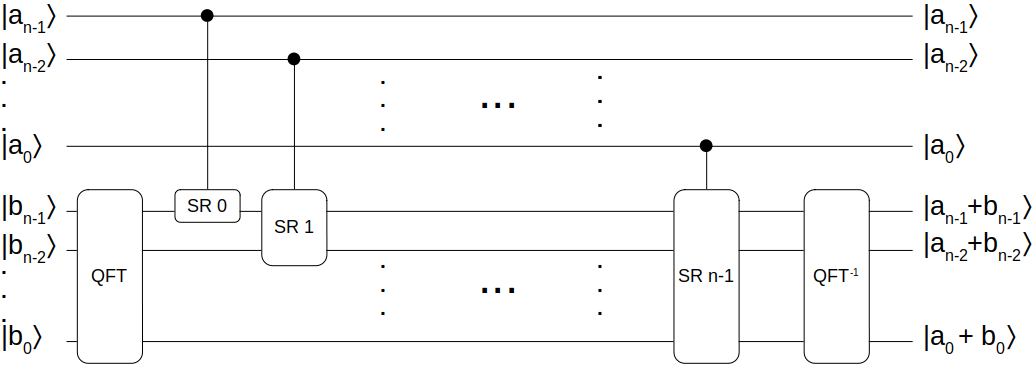
\includegraphics[width=1\textwidth]{qft-adder.png}
  \footnotesize
  \Qcircuit @C=0.25em @R=0.4em {
    \lstick{\qket{x_{n-1}}} & \multigate{4}{\texttt{$x-2^{I-i} n$}} & \multigate{4}{ \texttt{QFT}^{-1}\;N } & \ctrl{9} & \multigate{4}{ \texttt{QFT}\;N } & \multigate{4}{\texttt{$x+2^{I-i} n$}} & \qw & \qw & \qw \\
    \lstick{\qket{x_{n-2}}} &  \ghost{\texttt{$x-2^{I-i} n$}} & \ghost{ \texttt{QFT}^{-1}\;N } & \qw & \ghost{ \texttt{QFT}\;N } & \ghost{\texttt{$x+2^{I-i} n$}} & \qw & \qw & \qw \\
    \lstick{\vdots} & & & & & & & &  \rstick{\vdots} \\
    \lstick{} & &  & & & & & & \\
    \lstick{\qket{x_0}} & \ghost{\texttt{$x-2^{I-i} n$}}  & \ghost{ \texttt{QFT}^{-1}\;N } & \qw & \ghost{ \texttt{QFT}\;N } & \ghost{\texttt{$x+2^{I-i} n$}} & \qw & \qw & \qw  \\
\lstick{} & & & & & & & & &\\
    \lstick{\ket{b_{n-1}}} & \qw & \qw & \qw  & \qw & \qw & \qw & \qw & \qw   \\
    \lstick{\vdots} & & & & \dots &  & &   \\
    \lstick{} & & & & &  & & &   \\
    \lstick{\ket{b_{1}}} & \qw & \qw  &  \targ  & \qw & \ctrl{-5} & \qw & \targ & \qw   \\
    \lstick{\vdots} & & & & & & & &  \rstick{\vdots} \\
    \lstick{} & & & & & & & & &  \\
    \lstick{\ket{b_0}} & \qw & \qw & \qw & \qw & \qw & \qw & \qw & \qw  
    }
\subcaption{QFT-based}
\end{minipage} 
\\\\
\begin{minipage}{.7\textwidth}
% 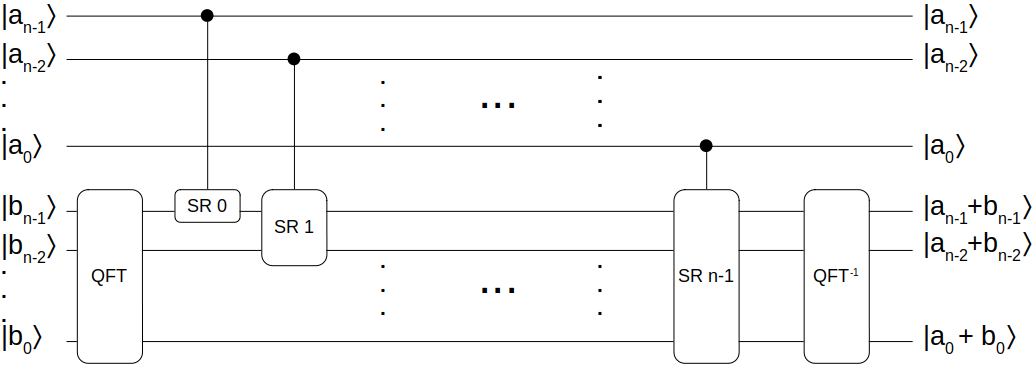
\includegraphics[width=1\textwidth]{qft-adder.png}
  \footnotesize
  \Qcircuit @C=0.25em @R=0.4em {
    \lstick{\qket{x_{n-1}}} & \multigate{4}{\texttt{$x-2^{I-i} n$}} & \multigate{4}{ \texttt{QFT}^{-1}\;(N-i) } & \qw & \qswap & \qw & \multigate{4}{ \texttt{RSH} } & \multigate{4}{ \texttt{QFT}\;(N-i-1) } & \multigate{4}{x+(2^{I-i} n \!\mod 2^{I-i-1})} & \qw & \qw & \qw & \qw  \\
    \lstick{\qket{x_{n-2}}} &  \ghost{\texttt{$x-2^{I-i} n$}} & \ghost{ \texttt{QFT}^{-1}\;(N-i) } & \qw & \qw \qwx &\qw & \ghost{ \texttt{RSH} } & \ghost{ \texttt{QFT}\;(N-i-1) } & \ghost{x+(2^{I-i} n \!\mod 2^{I-i-1})} & \qw & \qw & \qw & \qw \\
    \lstick{\vdots} & & & & \qwx & & & & & & & &  \rstick{\vdots} \\
    \lstick{} & &  & & \qwx & & & & & & & &  \\
    \lstick{\qket{x_0}} & \ghost{\texttt{$x-2^{I-i} n$}}  & \ghost{ \texttt{QFT}^{-1}\;(N-i) } & \qw & \qw \qwx & \qw & \ghost{\texttt{RSH}} & \ghost{ \texttt{QFT}\;(N-i-1) } & \ghost{x+(2^{I-i} n \!\mod 2^{I-i-1})} & \qw & \qw & \qw & \qw  \\
    \lstick{} & & & & \qwx & & & & & & & & & \\
    \lstick{\ket{b_{n-1}}} & \qw & \qw & \qw & \qw \qwx & \qw & \qw & \qw & \qw & \qw & \qw & \qw & \qw \\
    \lstick{\vdots} & & & & \qwx & & & \dots &  & & & & \\
    \lstick{} & & & & \qwx & & & & & & & & & \\
    \lstick{\ket{b_{1}}} & \qw & \qw  & \qw &  \qswap \qwx & \qw & \qw & \qw & \ctrl{-5} & \qw & \targ & \qw & \qw \\
    \lstick{\vdots} & & & & & & & & &&  & &  \rstick{\vdots} \\
    \lstick{} & & & & & & & & && & &  \\
    \lstick{\ket{b_0}} & \qw & \qw & \qw & \qw & \qw & \qw & \qw & \qw & \qw & \qw & \qw  & \qw 
    }
\subcaption{AQFT-based (addition and subtraction are approximate)}
\end{minipage} 
\end{tabular}
}
\caption{One step of the QFT/AQFT division/modulo circuit}
\label{fig:qft-moder}
\end{figure*}

\ignore{
\begin{figure*}[t]
\centering

\begin{coq}
Fixpoint appx_moder' i (n:nat) (b:nat) (x ex:var) (M:nat -> bool) := 
     match i with 0 =>  (SKIP (x,0))
           | S j => appx_compare_half3 x n b (ex,j) M ;  Rshift x;
                     QFT x b; (CU (ex,j) ((appx_adder x n b M)));
                      (X (ex,j)); 
                       appx_moder' j n (b+1) x ex (cut_n (div_two_spec M) n)
     end.
\end{coq}
\caption{Approximate QFT Modulo Operation (Core of Addition/Subtraction in \Cref{fig:circuit-add-sub})}
\label{fig:qft-moder}
\end{figure*}
}

Even though the approximate adder is not particularly useful for addition, there are still cases where it can be useful as a subcomponent. 
For example, the modulo/division circuit relies on an addition subcomponent, but does not need every bit to be correctly added.

\Cref{fig:qft-moder}(a) shows one step of an $N$-bit QFT-based modulo circuit that computes $x\!\!\mod n$ for constant $n$.
The algorithm runs for $I+1$ iterations, where $2^{N-1} \le 2^I n <2^N$, with the iteration counter $i$ increasing from 0 to $I$ (inclusive).
In each iteration, the circuit in \Cref{fig:qft-moder}(a) computes $x-2^{I-i} n$ and uses the result's most significant bit (MSB) to check whether $x < 2^{N-1-i}$.
If the MSB is $0$, then $x \ge 2^{N-1-i}$ and the circuit continues to next iteration; otherwise, it adds $2^{I-i} n$ to the result and continues.

We can improve the resource usage of the circuit in \Cref{fig:qft-moder}(a) by replacing the addition, subtraction, and QFT components with approximate versions, as shown in \Cref{fig:qft-moder}(b).
At the start of each iteration, $x < 2^{N-i}$, so it is safe to replace components with versions that will perform the intended operation on the lowest $(N-i)$ bits.
The circuit in \Cref{fig:qft-moder}(b) begins by subtracting the top $(N-i)$ bits, and then converts $x$ back to the \texttt{Nor} basis using an $(N-i)$-bit precision QFT\@.
It then swaps the MSB with an ancilla, guaranteeing that the MSB is 0. 
Next, it uses a \texttt{Rshift} to move the cleaned MSB to become the lowest significant bit (effectively, multiplying $x$ by 2) and uses a $(N-i-1)$-bit precision QFT to convert back to the \texttt{Phi} basis.
Finally, it conditionally adds back the top $(N-i-1)$ bit of the value $(2^{I-i} n \!\mod 2^{I-i-1})$, ignoring the original MSB.

The result is a division/modulo circuit that uses approximate components, but, as our testing assures, is exactly correct.
\Cref{fig:approx-results}(b) shows the required resources for varying numbers of iterations.
Compared to QFT-based circuit,
for a single iteration, the approximation provides a 4.5\% savings, and the saving increases with more iterations.
For $n = 1$, we need 16 iterations. In this case, the AQFT-based division/modulo circuit uses 61.1\% fewer gates than the QFT-based implementation.
If we compare the AQFT-based division/modulo circuit with the Toffoli-based one, the result is more significant. For 16 iterations, the AQFT-based division/modulo circuit uses 79.3\% fewer gates than the Toffoli-based implementation.

\section{Evaluation: \vqimp Oracles and Partial Evaluation}
\label{sec:partial-eval}

The prior section considered arithmetic operators implemented in
\oqasm. They are building blocks for operators we have programmed using
\vqimp, which include sine, 
arcsine, cosine, arccosine, and exponentiation on fixed-precision
numbers. We used \vqimp's source semantics to test each operator's
correctness.
These operators are useful in near-term applications; e.g., the
arcsine and sine functions are sub-components to repair the phase
values in constructing Hamiltonian simulations~\cite{feynman1982simulating} by the quantum walk
algorithm~\cite{Childs_2009}. 

As discussed in \Cref{sec:qimp}, one of the key features of \vqimp is \emph{partial evaluation} during compilation to \vqir.
The simplest optimization similar to partial evaluation happens for a
binary operation $x := x\odot y$, where $y$ is a constant value. 
\Cref{fig:circ-evaluation} hints at the power of partial evaluation for this case---all constant operations (marked ``const'') generate circuits with significantly fewer qubits and gates.
Languages like Quipper take advantage of this by producing special circuits for operations that use classically-known constant parameters.

Partial evaluation takes this one step further, pre-evaluating as much of the circuit as possible.
For example, consider the fixed precision operation $\frac{x*y}{M}$ where
$M$ is constant and a natural number, and $x$ and $y$ are two fixed precision numbers that may be constants.
This is a common pattern, appearing in many quantum oracles (recall the $\frac{8^n*x}{n!}$ in the Taylor series decomposition of sine). 
In Quipper, this is expression compiled to ${r_1}\texttt{ = }{\frac{x}{M}}; {r_2}\texttt{ = }{r1*y}$.
%
The \vqimp compiler produces different outputs depending on whether $x$ and $y$ are constants. If they both are constant, \vqimp simply assigns the result of computing $\frac{x*y}{M}$ to a quantum variable. If $x$ is a constant, but $y$ is not, \vqimp evaluates $\frac{x}{M}$ classically, assigns the value to $r_1$, and evaluates $r_2$ using a constant multiplication circuit. If they are both quantum variables, \vqimp generates a circuit to evaluate the division first and then the multiplication.

In \Cref{fig:self-data}~(a) we show the size of the circuit generated for $\frac{x*y}{M}$ where zero, one, or both variables are classically known. 
It is clear that more classical variables in a program lead to a more efficient output circuit.
If $x$ and $y$ are both constants, then only a constant assignment circuit is needed, which is a series of \texttt{X} gates. 
Even if only one variable is constant, it may lead to substantial savings: In this example, if $x$ is constant, the compiler can avoid the division circuit and use a constant multiplier instead of a general multiplier.
These savings quickly add up: \Cref{fig:self-data}~(b) shows the qubit size difference between our implementation of sine and Quippers'. Both the TOFF and QFT-based circuits use fewer than $7\%$ of the qubits used by Quipper's sine implementation.
\footnote{\vqimp also benefits from its representation of fixed-precision numbers (\Cref{sec:qimp}), which is more restrictive than Quipper's. Our representation of fixed-precision numbers reduces the qubit usage of the sine function by half, so about half of the qubit savings can be attributed to this.}

\begin{figure}[t]
{\small
\begin{subfigure}[b]{.6\textwidth}
\centering
\begin{tabular}{| l | c | c |}
\hline
                     & \# qubits  & \# gates   \\
                     \hline
OQIMP ($x$, $y$ const) & 16 & 16\\
OQIMP TOFF ($x$ const) & 33 & $1739 \pm 376$ \\
OQIMP QFT ($x$ const) & 16 & $1372 \pm 26$ \\
OQIMP TOFF & 33 & 61470   \\
OQIMP QFT & 32  & 25609  \\
\hline                           
\end{tabular}
  \subcaption{
Fixed-precision circuits for $\frac{x*y}{M}$ with $M=5$ (16 bits)
}
\end{subfigure}
\hfill
\begin{subfigure}[b]{.35\textwidth}
\centering
\begin{tabular}{| l | c|}
\hline
                     & \# qubits   \\
                     \hline
OQIMP TOFF & 418   \\
OQIMP QFT & 384  \\
Quipper & 6142  \\
\hline                           
\end{tabular}
  \subcaption{
Sine circuits (64 bits)}
\end{subfigure}
}
\caption{Effects of partial evaluation}
\label{fig:self-data}
\end{figure}

\section{Case Study: Grover's Search}
\label{sec:grovers}

Here we present a case study of integrating an oracle implemented with \name into a full quantum algorithm, Grover's search algorithm, implemented and verified in \sqir.

Grover's search algorithm \cite{grover1996,grover1997}, described in \Cref{sec:background}, has implications for cryptography, in part because it can be used to find collisions in cryptographic hash functions \cite{grover-hash}. Thus, the emergence of quantum computers may require lengthening hash function outputs.

We have used \vqimp to implement the ChaCha20 stream cipher \cite{chacha} as an oracle for Grover's search algorithm. 
%\name proved especially useful for this task, as \vqimp contains many of the operations commonly used by cryptographic hash functions, and any oracles were written can be efficiently tested on a classical machine.
%
This cipher computes a hash of a 256-bit key, a 64-bit message number, and a 64-bit block number, and it is actively being used in the TLS protocol \cite{rfc7905,rfc8446}.
The procedure consists of twenty cipher rounds, most easily implemented when segmented into quarter-round and double-round subroutines. 
The only operations used are bitwise \textsc{xor}, bit rotations, and addition modulo $2^{32}$, all of which are included in \vqimp; the implementation is given in \Cref{fig:chacha-qr}.

To test our oracle implementation, we wrote our specification as a Coq function on bitstrings.
We then defined correspondence between these bitstrings and program states in \vqir semantics and conjectured that for any inputs, the semantics of our compiled oracle matches the corresponding outputs from our specification function.
Using random testing (\Cref{sec:rand-testing}),
we individually tested the quarter-round and double-round subroutines as well as the whole twenty-round cipher, performing a sort of unit testing.
We also tested the oracle for the boolean-valued function that checks whether the ChaCha20 output matches a known bitstring rather than producing the output directly.
This oracle can be compiled to \sqir using our verified compiler, and then the compiled oracle can be used by Grover's algorithm to invert the ChaCha20 function and find collisions.
Grover's algorithm was previously implemented and verified in \sqir \cite{PQPC}, and we have modified this implementation and proof to allow for oracles with ancillae like the ones generated by our compiler; thus, our successful QuickChick tests combined with the previously proved theorems for Grover's algorithm provide confidence that we can find Chacha20's hash collisions in a certain probability through Grover's algorithm.

\begin{figure}[t]
\[\footnotesize
\begin{array}{l}
Q\;\tnat[4]\;qr(Q\;\tnat\;x_1,Q\;\tnat\;x_2,Q\;\tnat\;x_3,Q\;\tnat\;x_4)\;\{
\\
\quad{x_1}\texttt{ += }{x_2};\; {x_4}{\; \oplus\texttt{= } }{x_1};\; x_4\,\texttt{<{}<{}<=}\,16;\\
\quad{x_3}\texttt{ += }{x_4};\; {x_2}{\; \oplus\texttt{= } }{x_3};\; x_4\,\texttt{<{}<{}<=}\,12;\\
\quad{x_1}\texttt{ += }{x_2};\; {x_2}{\; \oplus\texttt{= } }{x_1};\; x_4\,\texttt{<{}<{}<=}\,8;\\
\quad{x_3}\texttt{ += }{x_4};\; {x_2}{\; \oplus\texttt{= } }{x_3};\; x_4\,\texttt{<{}<{}<=}\,7\\
\quad\texttt{return}\;[x_1,x_2,x_3,x_4];\\
\}\\\\
\texttt{void}\;chacha20(Q\;\tnat[16]\;x)\;\{
\\
\quad\texttt{for}(C\;\tnat\;i=20;\;i>0;\;i \texttt{ -= } 2)\;\{\\
\qquad [x[0], x[4], x[8], x[12]] = qr(x[0], x[4], x[8], x[12]);\\
\qquad [x[1], x[5], x[9], x[13]] = qr(x[1], x[5], x[9], x[13]);\\
\qquad [x[2], x[6], x[10], x[14]] = qr(x[2], x[6], x[10], x[14]);\\
\qquad [x[3], x[7], x[11], x[15]] = qr(x[3], x[7], x[11], x[15]);\\
\qquad [x[0], x[5], x[10], x[15]] = qr(x[0], x[5], x[10], x[15]);\\
\qquad [x[1], x[6], x[11], x[12]] = qr(x[1], x[6], x[11], x[12]);\\
\qquad [x[2], x[7], x[8], x[13]] = qr(x[2], x[7], x[8], x[13]);\\
\qquad [x[3], x[4], x[9], x[14]] = qr(x[3], x[4], x[9], x[14]);\\
\quad\}\\
\}
\end{array}
\]
\caption{ChaCha20 implementation in \vqimp}
\label{fig:chacha-qr}
\end{figure}

%\section{Related Work}
\label{sec:related}

\myparagraph{Oracles in Quantum Languages}

Quantum programming languages have proliferated in recent years. 
Many of these languages (e.g. Quil~\cite{quilc}, OpenQASM 2.0~\cite{Cross2017}, \sqir~\cite{VOQC}) describe low-level circuit programs and provide no abstractions for describing quantum oracles.
Higher-level languages may provide library functions for performing common oracle operations (e.g. Q\# \cite{qsharp}, Scaffold~\cite{scaffold,scaffCCnew}) or support compiling from classical programs to quantum circuits (e.g. Quipper~\cite{Green2013}), but still leave some important details (like uncomputation of ancilla qubits) to the programmer.

There has been some work on type systems to enforce that uncomputation happens correctly (e.g. Silq~\cite{sliqlanguage}), and on automated insertion of uncomputation circuits (e.g. Quipper~\cite{Green2013}, Unqomp~\cite{unqomp}), but while these approaches provide useful automation, they also lead to inefficiencies in compiled circuits.
For example, all of these tools force compilation into the classical gate set \texttt{X}, \texttt{CNOT},  and \texttt{CCNOT} (or ``Toffoli''), which precludes the use of QFT-based arithmetic, which uses fewer qubits than Toffoli-based approaches.
Of course, programmers are not obligated to use automation for constructing oracles---they can do it by hand for greater efficiency---but this risks mistakes.
\name allows programmers to produce oracles automatically from \vqimp using \texttt{inv} to uncompute, or to manually implement oracle functions in \vqir, in both cases supporting formal verification and testing.

% VARIOUS OLD TEXT:

% Quipper's approach is efficacious, but it can be inefficient and risks
% bugs. It compiles to a circuit whose gates do not leverage a quantum
% computer's specific capabilities. For example, addition between
% integers compiles to a classical ripple-carry adder rather than one
% based on the \emph{quantum fourier transform} (QFT), which can be more
% space-efficient. Quipper's compilation strategy also blows up the use
% of ancillae. For example, implementing cosine as a Haskell function
% and then building a Quipper circuit from it uses $n^2$ ancilla qubits
% for an $n$ qubit-encoded number, and usage increases linearly with the
% number of steps of the Taylor expansion. Of course, programmers are
% not obligated to use the above recipe for constructing oracles---they
% can do it by hand for greater efficiency---but this risks
% mistakes. While writing this paper we found a bug in Quipper's adder:
% When adding numbers of two different precisions, the lower-precision
% number is shifted incorrectly.\footnote{The \texttt{k} on the last line of
%   \texttt{qdouble\_align} should be \texttt{h}; \url{https://www.mathstat.dal.ca/~selinger/quipper/doc/src/Quipper/Algorithms/QLS/QDouble.html\#line-413}}

% \item Quipper~\cite{10.1145/2491956.2462177} -- see section 4.6. It
%   uses Template Haskell to take a Haskell function $f$ of type
%   \emph{list of bool} $\rightarrow$ \emph{list of bool} (or just a
%   single \emph{bool}), and converts it to $U_f$ for a fixed number of
%   qubits. A subsequent step ``uncomputes'' any ancillae that are no
%   longer needed. Note that Quipper has implemented \texttt{sin},
%   \texttt{cos}, etc. But: This is low-level, since the programmer must
%   manage lists of (physical) qubits and ancillae. No
%   verification. Look at current code and see what it can do now?

% Quipper \cite{Green2013} is a Haskell-like functional quantum language. Many quantum oracles have been defined in Quipper. Users are able to generate quantum circuits by using the Quipper compiler. We have mentioned several Quipper limitations in Sec.~\ref{sec:evaluation}. The major limitations are two. First, the circuits generated from Quipper oracles are not effective in terms of qubits and gates, and most Quipper oracle definitions are not verified. Quipper has a new development of compiling the language to QPMC \cite{Anticoli2017}, which is a model checker that is capable of verifying algorithms defined in Quipper. However, the oracles defined in Quipper are largely not verified. 

\myparagraph{Verified Quantum Programming}

Recent work on formally verifying quantum programs includes \qwire~\cite{RandThesis}, \sqir~\cite{PQPC}, and \qbricks~\cite{qbricks}. These tools have been used to verify a range of quantum algorithms, from Grover's search to quantum phase estimation.
Like these tools, properties of \vqir programs are expressed and verified in a proof assistant.
But, unlike these tools, we focus on a quantum sub-language that, while not able to express any quantum program, is efficiently simulatable.
This allows us to reuse existing infrastructure (like QuickChick~\cite{quickchick}) for testing Coq properties.

% We design \vqir with both efficiency and verification in mind:  on one hand, \vqir allows users to build more efficient quantum circuit constructions by leveraging native quantum operations such as Hadamard and quantum Fourier transformation; on the other hand, 
% we identify a class of such circuit constructions whose semantics can be succinctly expressed and efficiently simulated, the specific form of which is enforced by a type system on \vqir. 
% The latter eases the verification of the compilation and enables
% random testing, for any well-formed \vqir program.

\myparagraph{Verified Compilation of Quantum Programs}

Recent work has looked at verified optimization of quantum circuits (e.g., \voqc~\cite{VOQC}, CertiQ~\cite{Shi2019}), but the problem of verified \emph{compilation} from high-level languages to quantum circuits has received less attention.
The only examples of verified compilers for quantum circuits are ReVerC~\cite{reverC} and ReQWIRE~\cite{Rand2018ReQWIRERA}.
Both of these tools support verified translation from a low-level Boolean expression language to circuits consisting of \texttt{X}, \texttt{CNOT}, and \texttt{CCNOT} gates.
Compared to these tools, \name supports both a higher-level classical source language (\vqimp) and a more interesting quantum target language (\vqir).

% ReVerC \cite{reverC} is a language for writing reversible Boolean expressions by using \texttt{X}, \texttt{CNOT}, and \texttt{CCX} gates, which is similar to RKQC. It has a compiler to compile a relatively high-level reversible language (Revs) \cite{parent2015reversible} to circuits, and it is verified. The limitation of ReverC is that the language it supports is a relatively low-level Boolean expression language. Even though the compiler is verified and contains several examples of defining arithmetic operations, the operations are not verified yet. Additionally, ReverC is a reversible language and it does not provide a connection between quantum algorithms and quantum arithmetic oracles, as we did in Sec.~\ref{sec:grover-search}. 

% % Some prior work has also applied formal methods to compilation of
% % oracles. ReVerC is a formally verified compiler for reversible
% % circuits, but the input language is only boolean expressions, not
% % integers or decimal numbers, and compilation is only to classical
% % gates. ReQWIRE has similar limitations.

% \myparagraph{Entanglement in Quantum Languages}

% Quantum entanglement is an important feature of quantum programs, and also a useful tool for reasoning about quantum programs \cite{quantumseparation,Yuan2022}.
% Unfortunately, entanglement detection is at least an NP-hard problem \cite{entanglementdetection}.
% By design, an \oqasm program can never introduce entanglement.

%\section{Conclusion}

We present \name, a framework for expressing, testing, and verifying quantum oracles. The key component of \name is \vqir, the oracle quantum assembly language, which can express a restricted class of quantum programs that are efficiently simulatable (and hence testable) and are useful for implementing quantum oracles. 
We have verified the translator from \vqir to \sqir and have verified (or randomly tested) many arithmetic circuits written in \vqir.
We also present \vqimp, a high-level imperative language, and compiler from \vqimp to \vqir (framework verified and arithmetic operations randomly tested). We have used \name to implement oracles and oracle components useful in quantum programming, like modular multiplication and sine, and showed that our performance is comparable to the state-of-the-art (unverified) framework Quipper. We also demonstrated the benefit of partial evaluation in \vqimp, showing that partial evaluation results in our implementation of sine using just 7\% of the qubits used in Quipper's implementation.


%\section{RCIR+: its Type System and Semantics}
\label{sec:semantics}

As we have mentioned above, RCIR+ is a language for the purpose of compiling quantum oracle algorithms (or some other quantum algorithms, like Grover's algorithm, quantum walk and singular value transformation). Every quantum state in RCIR+ is represented by one of the three froms: $e^{\alpha}*|0>$ (or $e^{\alpha}*|1>$), $e^{\alpha}*(\pm|0>+\pm|1>)$, and $e^{\beta}*(|0> + e^{\alpha}*|1>)$. Based on the representation, we actually represent our quantum states as:

{
\[
rval = nat \to bool\qquad val = \texttt{nval}\; bool\;rval \;|\;\texttt{hval}\;bool\;bool\;rval\;|\;\texttt{qval}\;rval\;rval 
\]
}

Since all \texttt{Rz} gates in RCIR+ do rotations in the form either $2\pi i *\frac{1}{2^n}$ or $2\pi i *(1-\frac{1}{2^n})$, every angle rotation $\alpha$ in a state can be represented as a Boolean angle function $f$, whose meaning is defined as:

{
\[
 2\pi i * (\frac{1}{2^{1*(f(0))}} + \frac{1}{2^{2*(f(1))}} + ... + \frac{1}{2^{n*(f(n-1))}})
\]
}

\texttt{nval} is the state representation for $e^{\alpha}*|0>$ (or $e^{\alpha}*|1>$), and the Boolean value represents if the qubit state is $|0>$ or $|1>$. \texttt{hval} is the state representation for the form $e^{\alpha}*(\pm|0>+\pm|1>)$. The first Boolean value represents the $\pm$ sign for the $|0>$ qubit, and the second Boolean value represents the $\pm$ sign for the $|1>$ qubit. \texttt{qval} is to represent the states as the form $e^{\beta} * (|0> + e^{\alpha}*|1>)$. The first angle $rval$ represents $\beta$, while the second one represents $\alpha$ in the form with the semantic meaning described in the syntax above. In \texttt{Phi} mode, the only angle that can be rotated is $\alpha$.

For each state, we also have a type system to defines the type for it. The small type system has the following types:

\[
 type \;= \;\texttt{Nor}\; | \;\texttt{Had}\; |\; \texttt{Phi}\;nat
\]
 
The three different types refer to the three different modes of states described above. For a qubit state, it is impossible to have two kinds of states at the same time. \texttt{Nor} represents a state in \texttt{nval}, \texttt{Had} represents a state in \texttt{hval}, and \texttt{Phi} represents a state in \texttt{qval}. The natural number $nat$ associated with the \texttt{Phi} type represents the number of qubits that are related together in a QFT transformation. Turning a group of qubits to the \texttt{Phi} mode is essentially to do QFT on a group of qubits.  The type system will be associated with expressions in RCIR+. We first introduce the RCIR+ expressions here. Expressions in RCIR+ can be divided into three layers described in Fig.~\ref{fig:exp-layer}.

\begin{figure}[h]
\centering
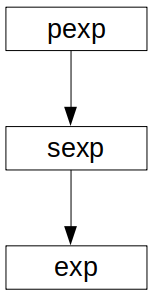
\includegraphics[width=0.15\textwidth]{exp_relation.png}
\caption{The Layer of Expressions in RCIR+}
\label{fig:exp-layer}
\end{figure}

The bottom level ($exp$) contains traditional quantum gates, like \texttt{X}, \texttt{CU}, \texttt{Rz} gates. On top of it, there is a set of operations ($sexp$) that deal with quantum state position swapping. Due to the virtual locations, the position swapping does not really have any effects in the actual physical quantum state locations. Instead, it changes the "view of qubits", which means we change the mapping from virtual state locations to physical locations. The top level ($pexp$) is to switch state space, which means that all operations there enforce certain type of state changes from one form to the other. We will discuss these expressions one by one. 

The syntax of the bottom level ($exp$) is described as follows:

\[
\begin{array}{l}
 exp \;= \texttt{SKIP}\; p \;|\; \texttt{X} \;p\; | \;\texttt{CU} \;p\; exp
        \;| \;\texttt{RZ} \;nat \;p
        \;|\; \texttt{RRZ} \;nat\; p 
\\\qquad
        \;|\; \texttt{SR}\; nat\; var
        \;|\; \texttt{SRR}\; nat\; var
        \;|\; \texttt{HCNOT} \;p\;p
        \;|\; \texttt{Seq} \;exp\; exp
\end{array}
\]

In $exp$, $p$ is a pair of a variable and a natural number. It represents the virtual location of a qubit state, and the application virtual location of a gate. The natural number ($n$, type: \texttt{nat}) appeared in the \texttt{RZ} and \texttt{RRZ} gates represents the rotation angle $2\pi i *\frac{1}{2^n}$ and $2\pi i *(1-\frac{1}{2^n})$, respectively. \texttt{RZ} represents actually the so-called \texttt{Rk} gate \cite{2000quant} in many traditional quantum gate descriptions, and \texttt{RRZ} is to apply an inverse \texttt{Rk} gate, which has the effect of applying the rotation $2\pi i *(1-\frac{1}{2^n})$ on the qubit state. 
\texttt{SR} gate is a special gate that is only used in \texttt{Phi} mode. It is actually a shortcut for a series of \texttt{RZ} gates. 
In \texttt{Phi} space, each qubit forms a suffix relation. In the first qubit in a \texttt{Phi} space, the $i$-th rotation position has to be the same as the $(i - m)$-th position for the $m$ qubit where $m\le i$. We call any of the rotation position across different qubits as linked rotation position. The \texttt{SR} gate is to enforce that every lined rotation position happened in \texttt{Phi} must rotate at the same angle every time. Otherwise, once we apply an inverted QFT after a rotation is applied to a \texttt{Phi} space, the system is not turned back to normal space. \texttt{SRR} is similar to \texttt{SR} but it contains a series of \texttt{RRZ} gates instead of \texttt{RZ} gates. \texttt{HCNOT} gate is essentially a \texttt{CNOT} gate with the restriction that the two positions must all in \texttt{Had} space. We will see examples of using these gates in the next section.

\begin{figure}[h]
\centering
\[\footnotesize
\begin{array}{l}
\begin{array}{llll}
\begin{array}{l}
\texttt{(1)}\;
\AxiomC{$$}
\UnaryInfC{$ \Gamma \vdash \texttt{SKIP}\;p$}
\DisplayProof
\end{array}
&
\begin{array}{l}
\texttt{(2)}\;
\AxiomC{$\Gamma(\texttt{fst}\;p)=\texttt{Nor}$}
\UnaryInfC{$ \Gamma \vdash \texttt{X}\;p$}
\DisplayProof
\end{array}
&
\begin{array}{l}
\texttt{(3)}\;
\AxiomC{$\Gamma(\texttt{fst}\;p)=\texttt{Had}$}
\UnaryInfC{$ \Gamma \vdash \texttt{X}\;p$}
\DisplayProof
\end{array}
&
\begin{array}{l}
\texttt{(4)}\;
\AxiomC{$\Gamma(\texttt{fst}\;p)=\texttt{Nor}\quad
 \Gamma\vdash e $}
\UnaryInfC{$ \Gamma \vdash \texttt{CU}\;p\;e$}
\DisplayProof
\end{array}
\end{array}
\\[2em]
\begin{array}{lll}
\begin{array}{l}
\texttt{(5)}\;
\AxiomC{$\Gamma(\texttt{fst}\;p_1)=\texttt{Had}\quad
 \Gamma(\texttt{fst}\;p_2)=\texttt{Had} $}
\UnaryInfC{$ \Gamma \vdash \texttt{CU}\;p_1\;p_2$}
\DisplayProof
\end{array}
&
\begin{array}{l}
\texttt{(6)}\;
\AxiomC{$\Gamma(\texttt{fst}\;p)=\texttt{Nor} $}
\UnaryInfC{$ \Gamma \vdash \texttt{RZ}\;q\;p$}
\DisplayProof
\end{array}
&
\begin{array}{l}
\texttt{(7)}\;
\AxiomC{$\Gamma(\texttt{fst}\;p)=\texttt{Had} $}
\UnaryInfC{$ \Gamma \vdash \texttt{RZ}\;1\;p$}
\DisplayProof
\end{array}
\end{array}
\\[2em]
\begin{array}{lll}
\begin{array}{l}
\texttt{(8)}\;
\AxiomC{$\Gamma(\texttt{fst}\;p)=\texttt{Nor} $}
\UnaryInfC{$ \Gamma \vdash \texttt{RRZ}\;q\;p$}
\DisplayProof
\end{array}
&
\begin{array}{l}
\texttt{(9)}\;
\AxiomC{$\Gamma(\texttt{fst}\;p)=\texttt{Had} $}
\UnaryInfC{$ \Gamma \vdash \texttt{RRZ}\;1\;p$}
\DisplayProof
\end{array}
&
\begin{array}{l}
\texttt{(10)}\;
\AxiomC{$\Gamma(x)=\texttt{Phi}\;n\quad
m<n $}
\UnaryInfC{$ \Gamma \vdash \texttt{SR}\;m\;x$}
\DisplayProof
\end{array}
\end{array}
\\[2em]
\begin{array}{ll}
\begin{array}{l}
\texttt{(11)}\;
\AxiomC{$\Gamma(x)=\texttt{Phi}\;n\quad
m<n $}
\UnaryInfC{$ \Gamma \vdash \texttt{SRR}\;m\;x$}
\DisplayProof
\end{array}
&
\begin{array}{l}
\texttt{(12)}\;
\AxiomC{$\Gamma \vdash \;e_1\quad \Gamma \vdash \;e_2 $}
\UnaryInfC{$ \Gamma \vdash \;\texttt{Seq}\;e_1\;e_2$}
\DisplayProof
\end{array}
\end{array}
\end{array}
\]
\caption{Well-Typed Definition For Exp}
\label{fig:exp-well-typed}
\end{figure}

The semantics of the expression is basically the same as ones appeared in SQIR. The only difference is that we are dealing with quantum states that are no entanglements. Therefore, the semantic description is more about to define the situation of applying different gates in the three modes of qubit states described above. The only tricky item here is that we have restrictions on the usage of different gates in different state modes. The relation that defines which gate is allowed to run on which mode is described in Fig.~\ref{fig:exp-well-typed}. In the figure, $\Gamma$ is a map from variables to modes. For example, \texttt{X} gates are allowed in the \texttt{Nor} and \texttt{Had} modes, while the control positions of \texttt{CU} gates are only allowed to run on the \texttt{Nor} mode, but the sub-expression of a \texttt{CU} gate can be run in other modes. \texttt{RZ} gate is fully allowed to run on the \texttt{Nor} mode, while if it is run on \texttt{Had}, the rotation angle is only allowed to be \texttt{1}, which means that the gate is a Pauli-Z gate. It is possible to extend the limitation to include \texttt{P} and \texttt{T} gates, but it will require more advanced state representation for \texttt{Had} mode. 
\texttt{SR} and \texttt{SRR} gates are \texttt{Phi} mode specific gates, while the two positions of \texttt{HCNOT} gates must be in the \texttt{Had} mode.

The second level expression ($sexp$) is mainly for swapping state positions. The syntax of $sexp$ is described as follows:

\[
sexp \;= \;\texttt{Lshift}\;x \;|\; \texttt{Rshift}\;x \;|\;\texttt{Rev}\;x 
                 \;|\; \texttt{Exp}\; exp \;|\; \texttt{SSeq} \;sexp\; sexp
\]

The variable $x$ in some expressions represents the virtual locations of a group of qubits. It has the same meaning as the first element of a pair $p$ appeared in $exp$. \texttt{Lshift} is to shift qubit virtual positions one step towards left for all qubits in $x$. If $x$ is allocated to have $n$ qubits, then, after the shift, the relation of the new state function $f'$ and the old one $f$ is: $f'(x,(i+1) \% n) = f(x,i)$ for $i=0,...,n-1$. \texttt{Rshift} is the opposite of \texttt{Lshift}, and the relation between $f'$ and old $f$ is: $f'(x,i) = f(x,(i+1)\%n)$ for $i=0,...,n-1$. \texttt{Rev} (the reverse operation) is to make the qubit positions up-side-down in $x$. Its semantic relation between $f'$ and old $f$ is given as: $f'(x,n-1-i) = f(x,i)$ for $i=0,...,n-1$.

The power of RCIR+ on dealing with these position swapping operations is that the compilations of these operations to SQIR all generate \textbf{zero} gates! During the compilation, instead of generating actually swap gates to do the operations, we actually change the mapping function from virtual qubit locations to its physical locations. For example, if we have a variable $x$ containing \texttt{4} qubits, and we applying a series of operations on it, such as $\texttt{SSeq}\;(\texttt{Lshift}\;x)\;e$. In this expression, $e$ is an expression that is applied to $x$ after the left-shift operation. Before applying the shift, let's assume that the compilation mapping is $\{(x,0) \mapsto 0, (x,1) \mapsto 1, (x,2) \mapsto 2, (x,3) \mapsto 3\}$. Then, after applying the shift, the compilation mapping becomes  $\{(x,3) \mapsto 0, (x,2) \mapsto 1, (x,1) \mapsto 2,(x,3) \mapsto 0\}$. Then, we also pass the mapping to deal with the applications in $e$. 

Since there is no \texttt{CU} gates in the $sexp$ and the top level, this mappings on each step can be generated during the program compilation time. One limitation is that, in RCIR+, one can never write a program with the \texttt{CU} gate on top of an expression containing these shift and reverse operations. We can call our shift/reverse operations as the static shift/reverse operations. If users really want the "dynamic" ones that live inside a \texttt{CU} gate, they can always define \texttt{SWAP} gates by using RCIR+. However, what we found out during the definition of the modulo-multiplication algorithm in RCIR+ is that we don't need to have "dynamic" shift/reserve operations and the static shift/reverse operations in RCIR+ can satisfy any needs in the algorithm. 

The top level expression ($pexp$) is to do another kind of "swapping" operations that swap/shift the qubit state modes, which is orthogonal with respect to the position swapping operations described above. The syntax of $pexp$ is described as follows:

\[
pexp \;=\; \texttt{SExp}\;sexp \;|\; \texttt{QFT} \;x \;| \;\texttt{RQFT}\; x
               \;|\; \texttt{H}\; x \;|\; \texttt{FSeq}\;pexp\;pexp
\]

\texttt{QFT} is to allow a quantum fourier transform (QFT) to all qubits in $x$, \texttt{RQFT} is the inverse QFT operation. \texttt{H} is a Hadamard gate. In the $sexp$ level, the types are actually not important since every shift/reverse operation can be applied in any mode. The types re-appear to be important in the $pexp$ level. The gates that live in this level actually shift the qubit state modes from one to the other. 

\begin{figure}[h]
\centering
\[\footnotesize
\begin{array}{l}
\begin{array}{ll}
\begin{array}{l}
\texttt{(13)}\;
\AxiomC{$\Gamma \vdash e$}
\UnaryInfC{$ (\Sigma,\Gamma) \vdash \texttt{SExp}\;e \triangleright \Gamma$}
\DisplayProof
\end{array}
&
\begin{array}{l}
\texttt{(14)}\;
\AxiomC{$\Gamma(x)=\texttt{Nor}\quad \Sigma(x)=n$}
\UnaryInfC{$ (\Sigma,\Gamma) \vdash \texttt{QFT}\;x\triangleright \Gamma[x\mapsto \texttt{Phi}\;n]$}
\DisplayProof
\end{array}
\end{array}
\\[2em]
\begin{array}{ll}
\begin{array}{l}
\texttt{(15)}\;
\AxiomC{$\Gamma(x)=\texttt{Phi}\;n$}
\UnaryInfC{$ (\Sigma,\Gamma) \vdash \texttt{RQFT}\;x\triangleright \Gamma[x\mapsto \texttt{Nor}]$}
\DisplayProof
\end{array}
&
\begin{array}{l}
\texttt{(16)}\;
\AxiomC{$\Gamma(x)=\texttt{Nor}\quad
 \Gamma\vdash e $}
\UnaryInfC{$ (\Sigma,\Gamma) \vdash \texttt{H}\;x\triangleright \Gamma[x\mapsto \texttt{Had}]$}
\DisplayProof
\end{array}
\end{array}
\\[2em]
\begin{array}{ll}
\begin{array}{l}
\texttt{(17)}\;
\AxiomC{$\Gamma(x)=\texttt{Had}$}
\UnaryInfC{$ (\Sigma,\Gamma) \vdash \texttt{H}\;x\triangleright \Gamma[x\mapsto \texttt{Nor}]$}
\DisplayProof
\end{array}
&
\begin{array}{l}
\texttt{(18)}\;
\AxiomC{$(\Sigma,\Gamma)\vdash e_1\triangleright \Gamma'
\quad(\Sigma,\Gamma')\vdash e_2\triangleright \Gamma'' $}
\UnaryInfC{$ (\Sigma,\Gamma) \vdash \texttt{FSeq}\;e_1\;e_2\triangleright \Gamma''$}
\DisplayProof
\end{array}
\end{array}
\end{array}
\]
\caption{Well-Typed Definition For PEXP}
\label{fig:pexp-well-typed}
\end{figure}

The well-typed definition for $pexp$ is listed in Fig.~\ref{fig:pexp-well-typed}. $\Sigma$ is an invariant map that records the number of qubits for each variable in the system. 
\texttt{QFT} can switch a state in the \texttt{Nor} mode to \texttt{Phi}, while \texttt{RQFT} can switch a state from \texttt{Phi} back to \texttt{Nor}. \texttt{H} gate switches the mode from \texttt{Nor} to \texttt{Had}, and switch a state in \texttt{Had} back to \texttt{Nor}.
The semantics of the $pexp$ gates has no essential difference from the same gates defined in SQIR. The only difference is that the gates are dealing with different qubit state representations than the ones in SQIR, and they also need to take care of mode switching.

\section{Example Quantum Circuits}
\label{sec:example}

In this section, we discuss the utility of RCIR+. As we mentioned above, we plan to utilize RCIR+ to analyze quantum circuits. The analysis means that doing property proofs, simulations, and random testing on quantum circuits. 
Here, we provide some example circuits that RCIR+ is capable of analyzing.

A trivial example of using RCIR+ is the ripple-carry adder \cite{ripple-carry}, since the gates used in the adder are essentially \texttt{X}, \texttt{CNOT}, and \texttt{CCX} gates, which are gates that can be analyzed in the \texttt{Nor} mode in RCIR+. 
A good example of using RCIR+ is probably the QFT-based arithmetic circuits. 

\begin{figure}[h]
\centering
     \begin{subfigure}[b]{0.6\textwidth}
         \centering
         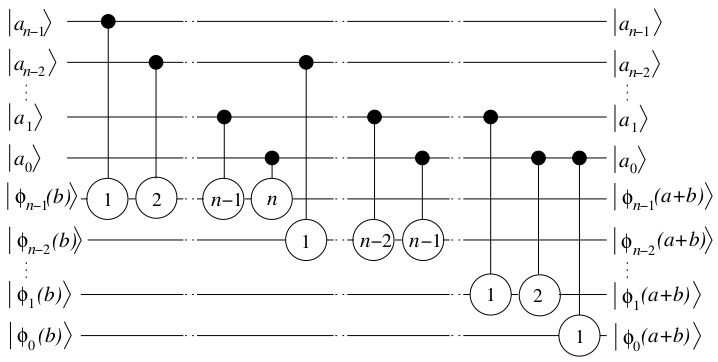
\includegraphics[width=1\textwidth]{qft-addition.png}
         \caption{QFT-based Addition Circuit}
         \label{fig:addition}
     \end{subfigure}%
     ~
     \begin{subfigure}[b]{0.6\textwidth}
         \centering
         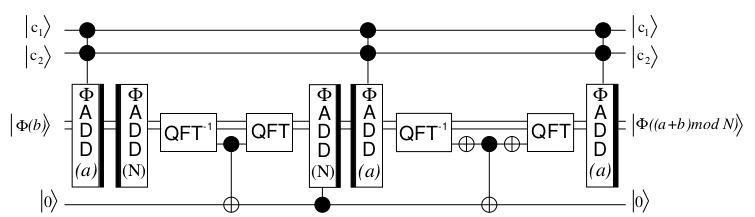
\includegraphics[width=1\textwidth]{qft-mod.png}
         \caption{QFT-based Modulo Multiplier Circuit}
         \label{fig:mod}
     \end{subfigure}

\caption{QFT-based Arithmetic Circuits}
\label{fig:qft-circuit}
\end{figure}

In Fig.~\ref{fig:qft-circuit}, we show the QFT-based addition circuit and a QFT-based modulo multiplier circuit. 
In Fig.~\ref{fig:addition}, the QFT-based addition circuit is assumed to have the input qubits for variable $b$ in the \texttt{Phi} mode, while qubits in variable $a$ are in the \texttt{Nor} mode.
To add the number $a$, which is represented as a binary Boolean values, to the $b$ value, it uses \texttt{CU} gates on variable $a$ qubits, and \texttt{RZ} gates for $b$. In RCIR+, we require gates in the \texttt{Phi} mode to only use \texttt{SR} and \texttt{SRR} gates. By exterminating the circuit carefully, we found that this is actually the case. For every qubit position $i$ in $a$, it touches only the $i$ rotation position in the rotation angle in each qubit of $b$. For example, the second $n-2$ qubit in $a$ rotates $\texttt{RZ}\;1$ in the $n-2$ qubit in $b$, and $\texttt{RZ}\;2$ in the $n-3$ qubit in $b$, and so on. We can conclude that an $n-i$ qubit in $a$ has \texttt{CU}-\texttt{RZ} gates on the $n-m$ qubit in $b$ where $m<i$, and the angle rotated in the $n-m$ qubit is $\texttt{RZ};(i-m+1)$. Hence, the \texttt{RZ} gates for each qubit in $a$ forms a \texttt{SR} gate in RCIR+. 
Fig.~\ref{fig:mod} show how to use mode transformation in RCIR+. We assume that the input for $b$ for the circuit is in the \texttt{Phi} mode, the two QFT-based addition circuits in the left can be done in the \texttt{Phi} mode, and the \texttt{RQFT} gate turns the mode of $b$ back to \texttt{Nor}, then it allows the \texttt{CNOT} gate (\texttt{CU} plus \texttt{X} gates) after \texttt{RQFT} is valid to run in the \texttt{Nor} mode. Then, the \texttt{QFT} gate turns $b$ back to \texttt{Phi}, and some other QFT-based addition operations can be applied on qubits in $b$. 

\begin{figure}[h]
\centering
         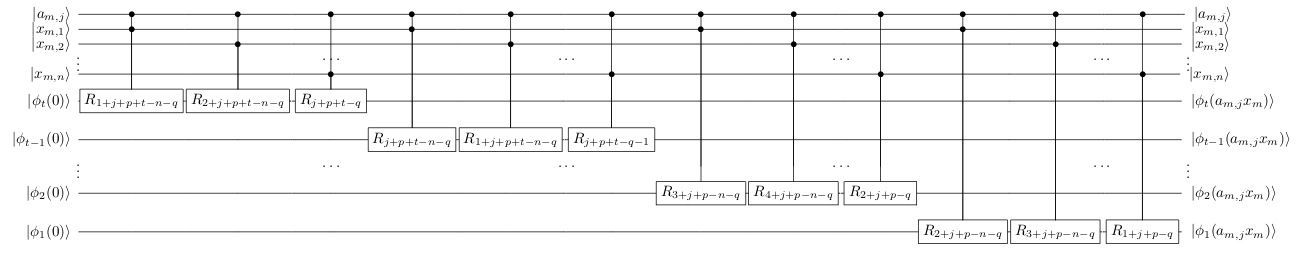
\includegraphics[width=\textwidth]{controlled-weight-sum.png}
\caption{QFT-based Controlled Weighted Sum Circuit}
\label{fig:qft-contol-circuit}
\end{figure}

Basically, all QFT-based arithmetic operations are analyzable by only using \texttt{SR} and \texttt{SRR} gates for \texttt{Phi}-mode qubits (obviously, we need other gates for qubits in the \texttt{Nor} mode). An example in the controlled weighted sum circuit in Fig.~\ref{fig:qft-contol-circuit}, which has the formula: $\Sigma^{2^n}_{m=1}a_m x_m$.

\begin{figure}[h]
\centering
     \begin{subfigure}[b]{0.6\textwidth}
         \centering
         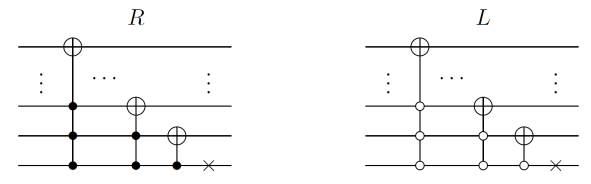
\includegraphics[width=1\textwidth]{lr-circuit.png}
         \caption{Circuits for L and R}
         \label{fig:lr-graph}
     \end{subfigure}

     \begin{subfigure}[b]{0.3\textwidth}
         \centering
         \includegraphics[width=1\textwidth]{circle-8-graph.png}
         \caption{Circle Graph (N = 8)}
         \label{fig:circle}
     \end{subfigure}%
     ~
     \begin{subfigure}[b]{0.7\textwidth}
         \centering
         \includegraphics[width=1\textwidth]{whole-quantum-walk.png}
         \caption{Full Circuit For Circle Graph Quantum Walk Oracle}
         \label{fig:quantum-walk-circle}
     \end{subfigure}

\caption{Quantum Walk Oracle Circuit}
\label{fig:circle-circuit}
\end{figure}

Another example circuit that can be analyzed is the oracle circuits in quantum walk in Fig.~\ref{fig:circle-circuit}. 
Most gates in the circuit are run in the \texttt{Nor} mode, and they can be analyzed by RCIR+. The only possible problem is the controlled-Z gate (\texttt{CZ}, listed as controlled $\pi$ in the Fig~\ref{fig:quantum-walk-circle}) surrounded by two \texttt{H} gates. In RCIR+, \texttt{CZ} gates are essentially \texttt{CU} gates and a $\texttt{RZ}$ gate with a rotation of angle $\pi$, and the \texttt{CU} gates are applied on qubits in \texttt{Nor}, as well as the \texttt{RZ} gate is applied on a qubit in the \texttt{Had} mode.
In Fig.~\ref{fig:quantum-walk-circle}, it seems that the \texttt{CZ} gate is applied on a controlled qubit in \texttt{Had} and all other qubits to be in \texttt{Nor}. What we find out is that these two \texttt{CZ} gate applications have the same effect. Any vector that is applied by a \texttt{CZ} gate where all controlled qubits are in \texttt{Nor} and the \texttt{RZ} applied qubit in the \texttt{Had} mode has the same effect as the one that is applied by a \texttt{CZ} gate where any one of the controlled qubit is in \texttt{Had} and all other qubits are in \texttt{Had}. This is why we are able to use RCIR+ to analyze the quantum walk oracle circuit in Fig.~\ref{fig:circle-circuit}.

\begin{figure}[h]
\centering
     \begin{subfigure}[h]{0.25\textwidth}
         \centering
         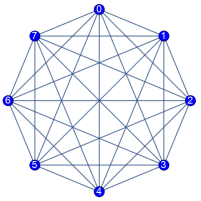
\includegraphics[width=1\textwidth]{k-graph.png}
     \end{subfigure}%
     ~
     \begin{subfigure}[h]{0.5\textwidth}
         \centering
         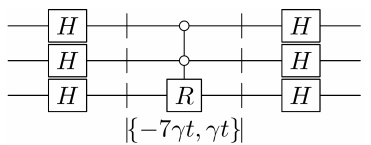
\includegraphics[width=1\textwidth]{tim-evolve-k-graph.png}
     \end{subfigure}
\caption{Quantum Walk Time-evolution Operator for $K_8$ Graph}
\label{fig:quantum-walk-time-evol}
\end{figure}

Unfortunately, not all quantum walk algorithm components are analyzable in RCIR+ with the qubit inputs to be in the \texttt{Nor} mode. 
Fig.~\ref{fig:quantum-walk-time-evol} shows a time-evolution operator in quantum walk for a $K_8$ graph.
This circuit is not analyzable in RCIR+ if the input qubits are in \texttt{Nor}.
To analyze this circuit in RCIR+, we first investigate an important theorem in dealing with quantum circuits in Observation~\ref{basic-state-thm}. 

\begin{observation}
\label{basic-state-thm}
\rm
If a quantum algorithm property is correct for all basis-vector inputs, the property can be extended for general quantum inputs.
\end{observation}

This Observation is a direct corollary from a theorem that is proved in the VOQC project \cite{10.1145/3434318}, where if two matrices produce the same output when they are multiplied by any basis-vector (a vector with $1$ in one row and $0$ in any other rows), then the two matrices are the same. An application of a quantum algorithm on an input is essentially to do a matrix multiplication on vectors as the input. The theorem tells us that if two algorithms are the same, then we only need to see if all basis-vectors as input for the two algorithms are the same. In contrast, if two quantum algorithms are tested to be the same under all basis-vectors, then we are not able to distinguish them by any input. In other word, if an algorithm property is correct in one algorithm $\sigma$, and there is another algorithm $\delta$ that is tested the same as $\sigma$ with all basis-vector inputs, then the property is also held in the algorithm $\delta$, because essentially algorithm properties are based on the input and output of algorithms. 

On the other hand, since all quantum algorithms are essentially matrix-vector multiplications, and any vectors can be viewed as a sum of scale multiplications of several basis vectors, if a property is held for all basis-vectors for an algorithm, the output behaviors of the property is calculable for arbitrary input vectors. 
This Observation can be extended to other forms of "basis" inputs for a quantum algorithms. Essentially, a basis-vector is a Kronecker product of qubits $|0>$ and $|1>$. One can produce a proportional relation between qubits $|+>$ ($\frac{1}{\sqrt{2}}(|0>+|1>)$) and $|->$ ($\frac{1}{\sqrt{2}}(|0>-|1>)$) are qubits $|0>$ and $|1>$. For example, $|0>\propto |+> + |->$. Hence, if a algorithm property is preserved for any Kronecker product of arbitrary $|+>$ and $|->$ (actually, we just need to analyze an arbitrary Kronecker product of exactly one $|->$ and many $|+>$), for arbitrary input qubits, the effects of the property is also calculable. 
For example, in dealing with the time-evolution operator in Fig.~\ref{fig:quantum-walk-time-evol}, if we assume that the input is an Kronecker product of $|+>$ and $|->$, then the inputs are in the \texttt{Had} mode, with the application of \texttt{H} gates, we can then analyze the effects of the \texttt{CU}-\texttt{RZ} gate in the middle. The quantum states to analyze in this format is a lot simpler than the ones if we assume that the input is with qubits $|0>$ and $|1>$. Additionally, if we keep the input as Kronecker products of $|+>$ and $|->$, in every computation step of the time-evolution operator, the quantum state is not entangled, which means that we can separately analyze every single qubit individually during the process. The direct consequence of analyzing the operator by using $|+>$ and $|->$ qubits is that we are able to design a traditional random testing algorithms to capture the behaviors for the time-evolution operator. We can then design the random testing kit in RCIR+ to have both inputs of Kronecker products of $|0>$ and $|1>$ (the \texttt{Nor} mode) and Kronecker products of $|+>$ and $|->$ (the \texttt{Had} mode) , so the random testing kit in RCIR+ now is able to show behaviors of more quantum algorithms. 

\begin{figure}[h]
\centering
         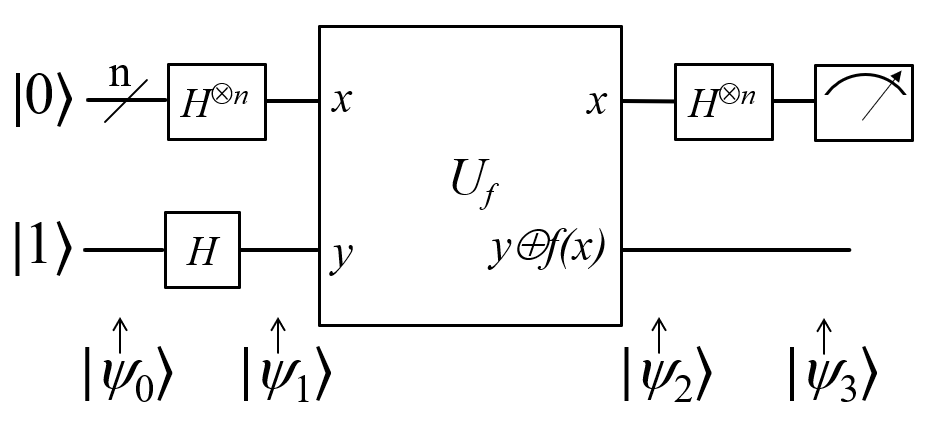
\includegraphics[width=0.5\textwidth]{deutsch-jozsa.png}
\caption{Deutsch-Jozsa Circuit}
\label{fig:Deutsch–Jozsa}
\end{figure}

A usage of the $|+>$/$|->$ qubit inputs is the analysis of the Deutsch–Jozsa algorithm (Fig.~\ref{fig:Deutsch–Jozsa}). By using the \texttt{Had} mode input, we are able to show the behaviors of step computations in this algorithm, and then for each step, we can produce the output behaviors of the algorithm with \texttt{Nor} mode input with a proper calculation. 

\section{An Example Usage of RCIR+: QSSA}
\label{sec:qssa}

One of the example usage of RCIR+ is the compilation of a high level SSA-formed (static single assignment formed) language with only arithmetic operations, such as math addition, subtraction, and multiplication, etc.

We first list the grammar of QSSA below:

\[
\begin{array}{l}
 fact \;= \texttt{Var}\; var \;|\; \texttt{Num} \;nat
\qquad
flag \;=\texttt{QFTA}\;|\;\texttt{Classic}
\qquad
bty\;=\texttt{Nat}\;|\;\texttt{Float}
\\[0.5em]
iexp \;=\texttt{plus}\;flag\;fact\;fact\;|\;\texttt{minus}\;flag\;fact\;fact\;|\;\texttt{mult}\;flag\;fact\;fact
\\\quad\;|\;\texttt{div}\;flag\;fact\;fact\;|\;\texttt{mod}\;flag\;fact\;fact\;|\;\texttt{load}\;var
\\[0.5em]
cexp \;=\texttt{clt}\;flag\;fact\;fact\;|\;\texttt{ceq}\;flag\;fact\;fact
\\[0.5em]
qexp\;=\texttt{inst}\;var\;nat\;bty\;iexp\;|\;\texttt{add}\;flag\;fact\;fact\;|\;\texttt{sub}\;flag\;fact\;fact
\\\quad\;|\;\texttt{times}\;flag\;fact\;fact
\;|\;\texttt{call}\;fvar
\;|\;\texttt{if}\;cexp\;qexp\;qexp
\;|\;\texttt{while}\;cexp\;qexp
\\\quad
\;|\;\texttt{ret}\;(list\;(var * var))
\;|\;\texttt{seq}\;qexp\;qexp
\\[0.5em]
fun\;=(fvar * qexp)
\qquad
prog\;=(nat * nat * nat * list\;(var * nat) * list\;fun)
\end{array}
\]

In QSSA, each variable is either a value representing a natural number (\texttt{Nat}) of a floating pointer number (\texttt{Float}). In addition, a variable can be either a global variable or a local variable. The expression \texttt{load} loads the value in a global variable to a local variable. The instruction \texttt{ret} returns a list of pairs of variables when a function is returned. In each pair $(x,u)$, $x$ must be a global variable and $u$ must be a local variable. The semantic meaning of \texttt{ret} for each pair $(x,u)$ is that $x:=u\oplus x$. From $iexp$, except \texttt{load}, all other expressions in QSSA are arithmetic operations. The $flag$ in each expression is either \texttt{QFTA} or \texttt{Classic}, meaning that the expression is computed using a QFT-based circuit and a classical circuit, respectively. $qexp$ represents instructions in a function. The basic instruction is $\texttt{inst}\;x\;n\;ty\;e$, where $x$ is the target variable to store the computation result, $n$ represents the number of bits in variable $x$, $ty$ defines if the value is a floating-point value or a natural number, and $e$ is an expression ($iexp$). All basic instructions $\texttt{inst}$ are required to be in SSA-format in a function, meaning that an variable $x$ in an \texttt{inst} can be assigned only once. For any \texttt{inst} having the form $x:=y\;\texttt{op}\;z$, it is corresponding to a reversible computation having the form as $[y][z][0]\rightarrow[y][z][x]$, where $x$ is the computation result of $y\;\texttt{op}\;z$.

In QSSA, we have a branching operation \texttt{if} and a loop operation \texttt{while}. Their Boolean guards are $cexp$ expressions. We currently allow users to compare if one value is smaller than the other one ($\texttt{clt}$), or if they are equal (\texttt{ceq}). 
In the body of a \texttt{while} loop in QSSA, we require that there is no basic instructions (\texttt{inst}). Instead, we provide three different operations for users in a loop body: \texttt{add}, \texttt{sub}, and \texttt{times}, with other kinds of instructions like \texttt{call}, \texttt{if}, \texttt{while}, \texttt{ret}, and \texttt{seq}. \texttt{add}, \texttt{sub}, and \texttt{times} represents math addition, subtraction, and multiplication, respectively. The difference between them and the ones in \texttt{inst} is the reversible computation formation. These three operations have the form: $[x][y]\rightarrow[x][y\;\texttt{op}\;x]$; so \texttt{add} can be better understood as "adding to", and \texttt{sub} is more like "subtracting from". We have the separation because of the efficiency concerns. Eventually, all variables in a QSSA function is mapped to an array of qubits. If we need to create a variable every time when a re-enter a loop body, this might not be feasible in the current status of a quantum circuit. Instead, most users might be interested in creating a variable before entering a loop, and updating the value in the variable when re-entering the loop. 
For each function ($fun$), there is also two global setting numbers that are related to the execution of a loop. The first number defines the stack size of a function, and the second number defines the maximum number of steps for executing a loop. The problem of having a loop in a quantum circuit is the loop Boolean guard. When executing a loop, every Boolean guard needs to be stored in a qubit, and for every step of computation, once a qubit is used for a Boolean guard, it cannot be re-used in the further step of loop-evaluation before the loop computation is finished. Hence, the compiler needs to know a place to swap clean ancillary qubits for storing a Boolean guard value.This is the so-called stack for a function, and the stack size for each function is pre-determined. In addition, for each loop execution, the maximum number of steps is also pre-determined, due to the fact that our compiler needs to expand the loop code before executing the loop operation.

In QSSA, function calls have no arguments at this point, and it is also not recursive. The usage of a function is to provide a automatic inverse circuit. For a function having the form: $f()\{e;\texttt{ret}\; l\}$, it is actually to execute the following: $e;\texttt{ret}\; l;\texttt{inv}\;e$. We first evaluate the function body $e$, and then the return instruction copies all local variables to global variables, and then we do an inverse of the function body $e$ (\texttt{inv}). 

Now, we discuss some about the compilation and type system of QSSA. Each variable in QSSA is having a type that is represented as a tuple of two different type fragments as: 

\[
\begin{array}{l}
bty\;=\texttt{Nat}\;|\;\texttt{Float}
\quad
aty\;=\texttt{C}\;nat\;|\;\texttt{Q}\;nat
\quad
type\;=(aty * bty)
\\[0.5em]
\end{array}
\]

Other than the \texttt{bty} fragment to classify if a variable representing a float or a natural number, the \texttt{aty} fragment checks if the value of a variable is "statically" determinable or "dynamically" determinable. 
The meaning of "statical"/"dynamical" determination is different from the version used in a classical compiler field. Here, we refer to statically determinable variable as its value is commutable without using quantum circuits, while dynamically determinable variable must hand to a quantum circuit to compute its value. The logic behinds this classification is that any effective computation that is compatible in a classical computer is a lot "cheaper" than doing the computation in a quantum machine.
The QSSA type system and compiler aggressively checks every line of code in a function and finds statically determinable variables as much as possible and per-compute all values for all statically determinable variables, and then we generate quantum circuits for only dynamical determinable variables.

A key observation of doing the compilation from QSSA to RCIR+ is that every operation in QSSA is a computation starting at a \texttt{Nor} mode and also ends at a \texttt{Nor} mode. If we think of the instruction in QSSA in terms of a compiled circuit in RCIR+, we find that the input for every operation is basically a series of qubits $|0>$ and $|1>$, and the output for every operation is also a series of $|0>$ and $|1>$. No matter the middle circuit is a QFT-based or a classical circuit, if the starting mode is \texttt{Nor}, then the ending mode is also \texttt{Nor}. This observation ease the compilation proofs from QSSA to RCIR+, and it also enables us to have a rich language representation.

One final thing worth noting is that QSSA is an example of using RCIR+. RCIR+ might enables more operations than the set of QSSA instructions listed here, such as the graph oracles and time evolving operators in quantum walk algorithms. For some enhanced quantum oracles or algorithm components, users might want to write their own effective circuit implementation in RCIR+. The RCIR+ random testing kit provides a way for helping users to validate and debug their large circuit implementations without going through the "pain" of proving the correctness of a compiler. 

\section{Evaluation and Future Study}
\label{sec:eval}
 
Currently, I have finished implementing the type system and semantics for RCIR+. I have already proved the correctness of compilation from RCIR+ to SQIR for $exp$ and $sexp$. I also the classical and QFT-based modulo multiplier on RCIR+, as well as the correctness proof for the classical modulo multiplier. There are several takeaways here. 

First, RCIR+ solves the problem of "can". By using RCIR+, we are able to define the classical and QFT-based adders and other oracle algorithms in a \textbf{single} framework. I also plan to define Grover's algorithm, as well as quantum walk algorithms in RCIR+. 
Second, RCIR+ also helps reduce the compilation gates. In dealing with the classical modulo multiplier, we are able to reduce 60\% of the
gates when we compile the circuit to SQIR. This is mainly because the fact that we don't need to do any static shift/reverse operations as well as reduce many swap operations. 
Third, RCIR+ helps the problem of "simplification". In defining the modes and restricting when a gate can be applied, we are able to avoid qubits having entanglements. This will certainly help simplifying the analysis of many quantum algorithms, especially oracle algorithm, that do not rely on entanglements. 
In addition, we can simplify the design of an RCIR+ simulator because the three different modes of qubit states that are based on natural numbers can improve the performance. 

For future study, I plan to define the sine/cosine functions based on the cordic method that relies on addition and shift operations, as well as many quantum oracles and components in quantum walk. Since I have finished the design for classical and QFT-based modulo multipliers, these automatically give us the addition, subtraction, and multiplication operations. These can be the basis of the compilation from QSSA to RCIR+. I can imagine the compilation will be easy to do since we have all separated components. Please feel free to talk to me and I need cooperation. 





%%Acknowledgments
\begin{acks}                            %% acks environment is optional
                                        %% contents suppressed with 'anonymous'
  %% Commands \grantsponsor{<sponsorID>}{<name>}{<url>} and
  %% \grantnum[<url>]{<sponsorID>}{<number>} should be used to
  %% acknowledge financial support and will be used by metadata
  %% extraction tools.
  % This material is based upon work supported by the
  % \grantsponsor{GS100000001}{National Science
  %   Foundation}{http://dx.doi.org/10.13039/100000001} under Grant
  % No.~\grantnum{GS100000001}{nnnnnnn} and Grant
  % No.~\grantnum{GS100000001}{mmmmmmm}.  Any opinions, findings, and
  % conclusions or recommendations expressed in this material are those
  % of the author and do not necessarily reflect the views of the
  % National Science Foundation.
We thank Leonidas Lampropoulos for helping us with effective use of
QuickChick, and Aaron Green and Robert Rand for helpful comments and contributions
during the development of this work. This material is based upon work supported
by the U.S. Department of 
Energy, Office of Science, Office of Advanced Scientific Computing
Research, Quantum Testbed Pathfinder Program under Award Number
DE-SC0019040, and the Air Force Office of Scientific Research under Grant No.
FA95502110051.
\end{acks}


%% Bibliography
\bibliography{reference}
\newpage
\section{\oqasm: An Assembly Language for Quantum Oracles}
\label{sec:vqir}

We designed \oqasm to be able to express efficient quantum
oracles that can be easily tested and, if desired, proved
correct.
\oqasm operations leverage both the standard
computational basis and an alternative basis connected by the quantum
Fourier transform (QFT). 
\oqasm's type system tracks the bases of variables in
\oqasm programs, forbidding operations that would introduce
entanglement. \oqasm states are therefore efficiently
represented, so programs can be effectively tested and are simpler to
verify and analyze. In addition, \oqasm uses \emph{virtual qubits}
to support \emph{position shifting operations}, which support
arithmetic operations without introducing extra gates during
translation. All of these features are novel to quantum assembly
languages. 

This section presents \oqasm states and the language's syntax,
semantics, typing, and soundness results.  As a running example, we use the QFT
adder~\cite{qft-adder} shown in \Cref{fig:circuit-example}. The Coq
function \coqe{rz_adder} generates an \oqasm program that adds two
natural numbers \coqe{a} and \coqe{b}, each of length \coqe{n} qubits.

\begin{figure*}[t]
  \centering
  \begin{tabular}{c @{\quad} c}
  \begin{minipage}[b]{.55\textwidth}
  % 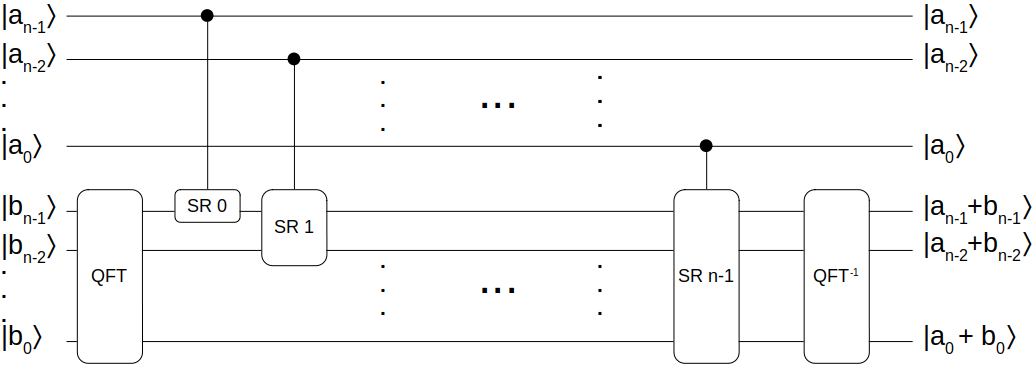
\includegraphics[width=1\textwidth]{qft-adder.png}
    \Small
    \Qcircuit @C=0.5em @R=0.75em {
      \lstick{\ket{a_{n-1}}} & \qw & \ctrl{5} & \qw & \qw & \qw & \qw & \qw & \qw & \qw & \rstick{\ket{a_{n-1}}} \\
      \lstick{\ket{a_{n-2}}} & \qw & \qw & \ctrl{4} & \qw & \qw & \qw & \qw & \qw & \qw & \rstick{\ket{a_{n-2}}}\\
      \lstick{\vdots} & & & & & & & & & & \rstick{\vdots} \\
      \lstick{} & & & & & & & & & & \\
      \lstick{\ket{a_0}} & \qw & \qw & \qw & \qw & \qw & \qw & \ctrl{1} & \qw & \qw & \rstick{\ket{a_0}} \\
      \lstick{\ket{b_{n-1}}} & \multigate{5}{\texttt{QFT}} & \gate{\texttt{SR 0}} & \multigate{3}{\texttt{SR 1}} & \qw & \qw & \qw & \multigate{5}{\texttt{SR (n-1)}} & \multigate{5}{\texttt{QFT}^{-1}} & \qw & \rstick{\ket{a_{n-1} + b_{n-1}}} \\
      \lstick{} & & & & & \dots & & & & \\
      \lstick{\ket{b_{n-2}}} & \ghost{\texttt{QFT}} & \qw  &  \ghost{\texttt{SR 1}} & \qw & \qw & \qw & \ghost{\texttt{SR (n-1)}} & \ghost{\texttt{QFT}^{-1}} & \qw & \rstick{\ket{a_{n-2} + b_{n-2}}} \\
      \lstick{\vdots} & & & & & & & & & & \rstick{\vdots} \\
      \lstick{} & & & & & & & & & & \\
      \lstick{\ket{b_0}} & \ghost{\texttt{QFT}} & \qw & \qw & \qw & \qw & \qw & \ghost{\texttt{SR (n-1)}} & \ghost{\texttt{QFT}^{-1}}  & \qw & \rstick{\ket{a_0 + b_0}} 
      }
  \subcaption{Quantum circuit}
  \end{minipage} &
  \begin{minipage}[b]{.35\textwidth}
  \begin{coq}
  Fixpoint rz_adder' (a b:var) (n:nat) 
    := match n with 
       | 0 => ID (a,0)
       | S m => CU (a,m) (SR m b); 
                rz_adder' a b m
       end.
  Definition rz_adder (a b:var) (n:nat) 
    := Rev a ; Rev b ; $\texttt{QFT}$ b ;
       rz_adder' a b n;
       $\texttt{QFT}^{-1}$ b; Rev b ; Rev a.
  \end{coq}
  \subcaption{\oqasm metaprogram (in Coq)}
  \end{minipage}
  \end{tabular}
  \vspace{-0.5em}
  \caption{Example \oqasm program: QFT-based adder}
  \label{fig:circuit-example}
  \end{figure*}

\subsection{\oqasm States} \label{sec:pqasm-states}

\begin{figure}[t]
  \small
  \[\hspace*{-0.5em}
\begin{array}{l>{$} p{1.2cm} <{$} c l}
      \text{Bit} & b & ::= & 0 \mid 1 \\
      \text{Natural number} & n & \in & \mathbb{N} \\
      \text{Real} & r & \in & \mathbb{R}\\
      \text{Phase} & \alpha(r) & ::= & e^{2\pi i r} \\
      \text{Basis} & \tau & ::= & \texttt{Nor} \mid \texttt{Phi}\;n \\
      \text{Unphased qubit} & \overline{q} & ::= & \ket{b} ~~\mid~~ \qket{r} \\
      \text{Qubit} & q & ::= &\alpha(r) \overline{q}\\
      \text{State (length $d$)} & \varphi & ::= & q_1 \otimes q_2 \otimes \cdots \otimes q_d
    \end{array}
  \]
  \caption{\oqasm state syntax}
  \label{fig:vqir-state}
\end{figure}

An \oqasm program state is represented according to the grammar in
\Cref{fig:vqir-state}. A state $\varphi$ of $d$ qubits is 
a length-$d$ tuple of qubit values $q$; the state models the tensor
product of those values. This means that the size of $\varphi$ is
$O(d)$ where $d$ is the number of qubits. A $d$-qubit state in a
language like \sqir is represented as a length $2^d$ vector of complex
numbers, which is $O(2^d)$ in the number of qubits.  Our linear state
representation is possible because applying any well-typed \oqasm
program on any well-formed \oqasm state never causes qubits to be
entangled.

A qubit value $q$ has one of two forms $\overline{q}$, scaled by a
global phase $\alpha(r)$. The two forms depend on the \emph{basis}
$\tau$ that the qubit is in---it could be either \texttt{Nor} or \texttt{Phi}. A \texttt{Nor} qubit has form
$\ket{b}$ (where $b \in \{ 0, 1 \}$), which is a
computational basis value. 
A \texttt{Phi} qubit has form $\qket{r} = \frac{1}{\sqrt{2}}(\ket{0}+\alpha(r)\ket{1})$, which is a value of the (A)QFT basis.
The number $n$ in \texttt{Phi}$\;n$ indicates the precision of the state $\varphi$.
As shown by~\citet{qft-adder}, arithmetic on the computational basis can sometimes be more efficiently carried out on the QFT basis, which leads to the use of quantum operations (like QFT) when implementing circuits with classical input/output behavior.
 
\subsection{\oqasm Syntax, Typing, and Semantics}\label{sec:oqasm-syn}

\liyi{add RZ gate back}

\begin{figure}[t]
\begin{minipage}[t]{0.5\textwidth}
{\small \centering

  $ \hspace*{-0.8em}
\begin{array}{llcl}
      \text{Position} & p & ::= & (x,n) \qquad   \text{Nat. Num}~n
                                  \qquad   \text{Variable}~x\\
      \text{Instruction} & \instr & ::= & \iskip{p} \mid \inot{p}
                                          \mid \irz[\lbrack -1 \rbrack]{n}{p} \mid \iseq{\instr}{\instr}\\
                & & \mid &  \isr[\lbrack -1 \rbrack]{n}{x} \mid \iqft[\lbrack -1 \rbrack]{n}{x} \mid \ictrl{p}{\instr}  \\
                      & & \mid & \ilshift{x} \mid \irshift{x} \mid \irev{x} 
    \end{array}
  $
}
  \caption{\oqasm syntax. For an operator \texttt{OP}, $\texttt{OP}^{\lbrack -1 \rbrack}$ indicates that the operator has a built-in inverse available.}
  \label{fig:vqir}
\end{minipage}
\hfill
\begin{minipage}[t]{0.45\textwidth}
\centering
\begin{tabular}{c@{$\quad=\quad$}c}
  \begin{minipage}{0.3\textwidth}
  \Small
%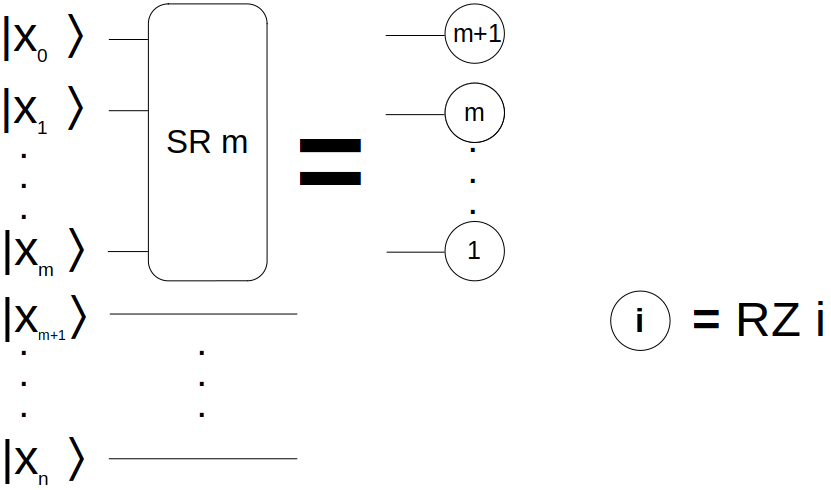
\includegraphics[width=0.3\textwidth]{sr-meaning.png}
  \Qcircuit @C=0.5em @R=0.5em {
    \lstick{} & \qw     & \multigate{4}{\texttt{SR m}} & \qw & \qw \\
    \lstick{} & \qw     & \ghost{\texttt{SR m}}           & \qw & \qw \\
    \lstick{} & \vdots & & \vdots & \\
    \lstick{} & & & & \\
    \lstick{} & \qw     & \ghost{\texttt{SR m}}           & \qw  & \qw
    }
  \end{minipage} & 
  \begin{minipage}{0.3\textwidth}
  \Small
  \Qcircuit @C=0.5em @R=0.5em {
    \lstick{} & \qw     & \gate{\texttt{RZ (m+1)}} & \qw & \qw \\
    \lstick{} & \qw     & \gate{\texttt{RZ m}}          & \qw & \qw \\
    \lstick{} & & \vdots & & \\
    \lstick{} & & & & \\
    \lstick{} & & & & \\
    \lstick{} & \qw     & \gate{\texttt{RZ 1}}           & \qw  & \qw
    }
  \end{minipage} 
\end{tabular}
\caption{\texttt{SR} unfolds to a series of \texttt{RZ} instructions}
\label{fig:sr-meaning}
\end{minipage}
\end{figure}

\Cref{fig:vqir} presents \oqasm's syntax. An \oqasm program consists of
a sequence of instructions $\instr$. Each instruction applies an
operator to either a variable $x$, which represents a group of qubits,
or a \emph{position} $p$, which identifies a particular offset into a variable $x$. 

The instructions in the first row correspond to simple single-qubit
quantum gates---$\iskip{p}$, $\inot{p}$, and $\irz[\lbrack -1 \rbrack]{n}{p}$
 ---and instruction sequencing.
The instructions in the next row apply to whole variables: $\iqft{n}{x}$
applies the AQFT to variable $x$ with $n$-bit precision and
$\iqft[-1]{n}{x}$ applies its inverse.
If $n$ is equal to the size of $x$, then the AQFT operation is exact.
$\isr[\lbrack -1 \rbrack]{n}{x}$
applies a series of \texttt{RZ} gates (\Cref{fig:sr-meaning}). 
Operation $\ictrl{p}{\instr}$
applies instruction $\instr$ \emph{controlled} on qubit position
$p$. All of the operations in this row---\texttt{SR}, \texttt{QFT}, and \texttt{CU}---will be translated to multiple \sqir
gates. Function \coqe{rz_adder} in \Cref{fig:circuit-example}(b) uses
many of these instructions; e.g., it uses \texttt{QFT} and \texttt{QFT}$^{-1}$ and applies
\texttt{CU} to the $m$th position of variable \texttt{a} to control
instruction \texttt{SR m b}.

In the last row of \Cref{fig:vqir}, instructions $\ilshift{x}$,
$\irshift{x}$, and $\irev{x}$ are \emph{position shifting operations}.
Assuming that $x$ has $d$ qubits and $x_k$ represents the $k$-th qubit
state in $x$, $\texttt{Lshift}\;x$ changes the $k$-th qubit state to
$x_{(k + 1)\% d}$, $\texttt{Rshift}\;x$ changes it to
$x_{(k + d - 1)\% d}$, and \texttt{Rev} changes it to $x_{d-1-k}$. In
our implementation, shifting is \emph{virtual} not physical. The \oqasm
translator maintains a logical map of variables/positions to concrete
qubits and ensures that shifting operations are no-ops, introducing no extra gates.

Other quantum operations could be added to \oqasm to
allow reasoning about a larger class of quantum programs, while still
guaranteeing a lack of entanglement. In \Cref{sec:extended-oqasm}, we
show how \oqasm can be extended to include the Hadamard gate
\texttt{H}, $z$-axis rotations \texttt{Rz}, and a new basis
\texttt{Had} to reason directly about implementations of QFT and AQFT\@.
However, this extension compromises the property of type reversibility
(\Cref{thm:reversibility}, \Cref{sec:metatheory}), and we have not found it necessary in
oracles we have developed.

\begin{figure}[t]
\begin{minipage}[t]{0.6\textwidth}
{\Small
  \begin{mathpar}
    \inferrule[X]{\Omegaty(x)=\texttt{Nor} \\ n < \Omegasz(x)}{\Sigma;\Omega \vdash \inot{(x,n)}\triangleright \Omega}
  
    \inferrule[RZ]{\Omegaty(x)=\texttt{Nor} \\ n < \Omegasz(x)}{\Sigma;\Omega \vdash \irz{q}{(x,n)} \triangleright \Omega}

    \inferrule[SR]{\Omegaty(x)=\tphi{n} \\ m < n}{\Sigma;\Omega \vdash \texttt{SR}\;m\;x\triangleright \Omega}   

    \inferrule[QFT]{\Omegaty(x)=\texttt{Nor}\\n \le \Omegasz(x)}{\Sigma; \Omega \vdash \iqft{n}{x}\triangleright \Omega[x\mapsto \tphi{n}]}    
     
    \inferrule[RQFT]{\Omegaty(x)=\tphi{n}\\n \le \Omegasz(x)}{\Sigma; \Omega \vdash \iqft[-1]{n}{x}\triangleright \Omega[x\mapsto \texttt{Nor}]}             
    
    \inferrule[CU]{\Omegaty(x)=\texttt{Nor} \\ \texttt{fresh}~(x,n)~\instr \\\\ \Sigma; \Omega\vdash \instr\triangleright \Omega \\ \texttt{neutral}(\instr)}{\Sigma; \Omega \vdash \texttt{CU}\;(x,n)\;\instr \triangleright \Omega} 
     
    \inferrule[LSH]{\Omegaty(x)=\texttt{Nor}}{\Sigma; \Omega \vdash \texttt{Lshift}\;x\triangleright \Omega}

     \inferrule[SEQ]{\Sigma; \Omega\vdash \instr_1\triangleright \Omega' \\ \Sigma; \Omega'\vdash \instr_2\triangleright \Omega''}{\Sigma; \Omega \vdash \instr_1\;;\;\instr_2\triangleright \Omega''} 
    
  \end{mathpar}
}
  \caption{Select \oqasm typing rules}
  \label{fig:exp-well-typed}
\end{minipage}
\hfill
\begin{minipage}[t]{0.35\textwidth}
{\footnotesize
\begin{center}\hspace*{-1em}
\begin{tikzpicture}[->,>=stealth',shorten >=1pt,auto,node distance=3.2cm,
                    semithick]
  \tikzstyle{every state}=[fill=black,draw=none,text=white]

  \node[state] (A)              {$\texttt{Nor}$};
  \node[state]         (C) [left of=A] {$\tphi{n}$};

  \path (A) edge [loop above]            node {$\Big\{\begin{array}{l}\texttt{ID},~\texttt{X},~\texttt{RZ}^{\lbrack -1 \rbrack},~\texttt{CU},\\
              \texttt{Rev},\texttt{Lshift},\texttt{Rshift}\end{array}\Big\}$} (A)
            edge   node [above] {\{$\texttt{QFT}\;n$\}} (C);
  \path (C) edge [loop above]            node {$\{\texttt{ID},~\texttt{SR}^{\lbrack -1 \rbrack}\}$} (C)
            edge  [bend right]             node {$\{\texttt{QFT}^{-1}\;n\}$} (A);
\end{tikzpicture}
\end{center}
}
\caption{Type rules' state machine}
\label{fig:state-machine}
\end{minipage}
\end{figure}

\myparagraph{Typing}
\label{sec:vqir-typing}

In \oqasm, typing is with respect to a \emph{type environment}
$\Omega$ and a predefined \emph{size
  environment} $\Sigma$, which map \oqasm
variables to their basis and size (number of qubits), respectively.
The typing judgment is written $\Sigma; \Omega\vdash \instr \triangleright \Omega'$ which
states that $\instr$ is well-typed under $\Omega$ and $\Sigma$, and
transforms the variables' bases to be as in $\Omega'$ ($\Sigma$ is unchanged). 
\liyi{good?}
$\Sigma$ is fixed because the number of qubits in an execution is always fixed.
It is generated in the high level language compiler, such as \sourcelang in \Cref{sec:qimp}.
The algorithm generates $\Sigma$ by taking an \sourcelang program and scanning through
all the variable initialization statements.
Select type rules are given in \Cref{fig:exp-well-typed}; 
the rules not shown (for \texttt{ID}, \texttt{Rshift}, \texttt{Rev}, \texttt{RZ}$^{-1}$, and \texttt{SR}$^{-1}$) are similar.

The type system enforces three invariants.  First, it enforces that
instructions are well-formed, meaning that gates are applied to valid
qubit positions (the second premise in \rulelab{X}) and that any control qubit is distinct from the
target(s) (the \texttt{fresh} premise in
\rulelab{CU}).  This latter property enforces the quantum
\emph{no-cloning rule}.
For example, we can apply the \texttt{CU} in \code{rz\_adder'} (\Cref{fig:circuit-example})
because position \code{a,m} is distinct from variable \code{b}.

Second, the type system enforces that instructions leave affected
qubits in a proper basis (thereby avoiding entanglement). The
rules implement the state machine shown in
\Cref{fig:state-machine}. For example, $\texttt{QFT}\;n$ transforms a variable from \texttt{Nor} to
$\tphi{n}$ (rule \rulelab{QFT}), while $\texttt{QFT}^{-1}\;n$
transforms it from $\tphi{n}$ back to \texttt{Nor} (rule
\rulelab{RQFT}). Position shifting operations 
are disallowed on variables $x$ in
the \texttt{Phi} basis because the qubits that make up $x$ are
internally related (see \Cref{def:well-formed}) and cannot be rearranged. Indeed, applying a
\texttt{Lshift} and then a $\texttt{QFT}^{-1}$ on $x$ in \texttt{Phi}
would entangle $x$'s qubits.

% \begin{figure}[t]
% {\footnotesize
% \begin{center}
% \begin{tikzpicture}[->,>=stealth',shorten >=1pt,auto,node distance=3.2cm,
%                     semithick]
%   \tikzstyle{every state}=[fill=white,draw=black,text=black]
% 
%   \node[initial,accepting,state] (A)              {$\texttt{OK}$};
%   \node[state]         (B) [right of=A] {$ $};
% 
%   \path (A) edge [loop above]            node {$b,\epsilon / \epsilon$} (A)
%             edge  [above] node {$a,\emptyset / a$} (B);
%   \path (B) edge [loop right]            node [right] {$\begin{array}{l}b,\epsilon / \epsilon\\
%                                                                 a,a' / a a'\\
%                                                                 a,\overline{a} / \epsilon\\
%                                                  \end{array}$} (B)
%             edge  [bend left]             node [above] {$\epsilon,\emptyset / \emptyset$} (A);
% \end{tikzpicture}
% \end{center}
% }
% {
% \footnotesize
% $
% \begin{array}{l}
% a,a'\in \{\ilshift{x},\irshift{x},\irev{x} \} \wedge a' \neq \overline{a}
% \\
% \overline{\ilshift{x}}=\irshift{x}
% \quad
% \overline{\irshift{x}}=\ilshift{x}
% \quad
% \overline{\irev{x}}=\irev{x}
% \\
% b\not\in\{\ilshift{x},\irshift{x},\irev{x}, \instr;\instr \}
% \\
% \emptyset=\text{ no element in stack}
% \end{array}
% $
% }
% 
% \caption{Pushdown automata for \texttt{neutral}}
% \label{fig:pushdown-neu}
% \end{figure}

Third, the type system enforces that the effect of position shifting
operations can be statically tracked. The \texttt{neutral} condition of
\rulelab{CU} requires that any shifting within $\instr$ is restored by the time it
completes. 
For example, $\sseq{\ictrl{p}{(\ilshift{x})}}{\inot{(x,0)}}$ is not well-typed, because knowing the final physical position of qubit $(x,0)$ would require statically knowing the value of $p$. 
On the other hand, the program $\sseq{\ictrl{c}{(\sseq{\ilshift{x}}{\sseq{\inot{(x,0)}}{\irshift{x}}})}}{\inot{(x,0)}}$ is well-typed 
because the effect of the \texttt{Lshift} is ``undone'' by an \texttt{Rshift} inside the body of the \texttt{CU}.

% \texttt{neutral}'s definition in \Cref{fig:pushdown-neu}
% views $\instr$ as a string concatenated
% by the sequence operation ($;$) and requires $\instr$ to be
% accepted according to a family of pushdown automatas $\{G\}_{x}$ for every $x$ presented in $\instr$. 
% A program $\instr$ is \texttt{neutral}, iff, $\instr$ as a string is
% accepted by all the automatas in $\{G\}_{x}$.

\myparagraph{Semantics}\label{sec:pqasm-dsem}

\begin{figure}[t]
{\footnotesize
\[
\begin{array}{lll}
\llbracket \iskip{p} \rrbracket\varphi &= \varphi\\[0.2em]

\llbracket \inot{(x, i)} \rrbracket\varphi &= \app{\uparrow\xsem(\downarrow\varphi(x,i))}{\varphi}{(x,i)}
& \texttt{where  }\xsem(\ket{0})=\ket{1} \qquad\, \xsem(\ket{1})=\ket{0}
\\[0.5em]

\llbracket \ictrl{(x,i)}{\instr} \rrbracket\varphi &=  \csem(\downarrow\varphi(x,i),\instr,\varphi)
&
\texttt{where  }
\csem({\ket{0}},{\instr},\varphi)=\varphi\quad\;\,
\csem({\ket{1}},{\instr},\varphi)=\llbracket \instr \rrbracket\varphi
\\[0.4em]

\llbracket \irz{m}{(x,i)} \rrbracket\varphi &= \app{\uparrow {\rsem}({m},\downarrow\varphi(x,i))}{\varphi}{(x,i)}
&\texttt{where  }{\rsem}(m,\ket{0})=\ket{0} \; \quad{\rsem}(m,\ket{1})=\alpha(\frac{1}{2^m})\ket{1}
\\[0.5em]

\llbracket \irz[-1]{m}{(x,i)} \rrbracket\varphi &= \app{\uparrow {\rrsem}({m},\downarrow\varphi(x,i))}{\varphi}{(x,i)}
 &\texttt{where  }{\rrsem}(m,\ket{0})=\ket{0}
\quad{\rrsem}(m,\ket{1})=\alpha(-\frac{1}{2^m})\ket{1}
\\[0.5em]

\llbracket \isr{m}{x} \rrbracket\varphi &
                                            \multicolumn{2}{l}{= \app{\uparrow \qket{r_i+\frac{1}{2^{m-i+1}}}}{\varphi}{\forall i \le m.\;(x,i)}
\qquad \texttt{when  }
\downarrow\varphi(x,i) = \qket{r_i}}\\[0.5em]

\llbracket \isr[-1]{m}{x} \rrbracket\varphi&\multicolumn{2}{l}{= \app{\uparrow \qket{r_i-\frac{1}{2^{m-i+1}}}}{\varphi}{\forall i \le m.\;(x,i)}
\qquad \texttt{when  }
\downarrow\varphi(x,i) = \qket{r_i}}\\[0.5em]

\llbracket \iqft{n}{x} \rrbracket\varphi &= \app{\uparrow\qsem(\Sigma(x),\downarrow\varphi(x),n)}{\varphi}{x}
& \texttt{where  }\qsem(i,\ket{y},n)=\bigotimes_{k=0}^{i-1}(\qket{\frac{y}{2^{n-k}}})
\\[0.5em]

\llbracket \iqft[-1]{n}{x} \rrbracket\varphi &=  \app{\uparrow\qsem^{-1}(\Sigma(x),\downarrow\varphi(x),n)}{\varphi}{x}
\\[0.5em]

\llbracket \ilshift{x} \rrbracket\varphi &= \app{{\psem}_{l}(\varphi(x))}{\varphi}{x}
&
\texttt{where  }{\psem}_{l}(q_0\otimes q_1\otimes \cdots \otimes q_{n-1})=q_{n-1}\otimes q_0\otimes q_1 \otimes \cdots
\\[0.5em]

\llbracket \irshift{x} \rrbracket\varphi &= \app{{\psem}_{r}(\varphi(x))}{\varphi}{x}
&
\texttt{where  }{\psem}_{r}(q_0\otimes q_1\otimes \cdots \otimes q_{n-1})=q_1\otimes \cdots \otimes q_{n-1} \otimes q_0
\\[0.5em]

\llbracket \irev{x} \rrbracket\varphi &= \app{{\psem}_{a}(\varphi(x))}{\varphi}{x}
&
\texttt{where  }{\psem}_{a}(q_0\otimes \cdots \otimes q_{n-1})=q_{n-1}\otimes \cdots \otimes q_0
\\[0.5em]

\llbracket \iota_1; \iota_2 \rrbracket\varphi &= \llbracket \iota_2 \rrbracket (\llbracket \iota_1 \rrbracket\varphi)
\end{array}
\]
}
{\footnotesize
$
\begin{array}{l}
\\[0.2em]
\downarrow \alpha(b)\overline{q}=\overline{q}
\qquad
\downarrow (q_1\otimes \cdots \otimes q_n) = \downarrow q_1\otimes \cdots \otimes \downarrow q_n
\\[0.2em]
\app{\uparrow \overline{q}}{\varphi}{(x,i)}=\app{\alpha(b)\overline{q}}{\varphi}{(x,i)}
\qquad \texttt{where  }\varphi(x,i)=\alpha(b)\overline{q_i}
\\[0.2em]
\app{\uparrow \alpha(b_1)\overline{q}}{\varphi}{(x,i)}=\app{\alpha(b_1+b_2)\overline{q}}{\varphi}{(x,i)}
\qquad \texttt{where  }\varphi(x,i)=\alpha(b_2)\overline{q_i}
\\[0.2em]
\app{q_x}{\varphi}{x}=\app{q_{(x,i)}}{\varphi}{\forall i < \Sigma(x).\;(x,i)}
\\[0.2em]
\app{\uparrow q_x}{\varphi}{x}=\app{\uparrow q_{(x,i)}}{\varphi}{\forall i < \Sigma(x).\;(x,i)}
\end{array}
$
}
\vspace*{-0.5em}
\caption{\oqasm semantics}
  \label{fig:deno-sem}
\end{figure}

We define the semantics of an \oqasm program as a partial function
$\llbracket\rrbracket$ from
an instruction $\instr$ and input state $\varphi$ to an output state
$\varphi'$, written 
$\llbracket \instr \rrbracket\varphi=\varphi'$, shown in \Cref{fig:deno-sem}.
% The definition for $\llbracket\rrbracket$ is syntax-driven, meaning that it is defined in terms of the state syntax presented in \Cref{fig:vqir-state}.

% defines the denotational semantics of \oqasm, which maps a \oqasm instruction $\instr \in \{\instr\}$ to its unitary operator on $\varphi \in \hsp{S}^d$.

% The key takeaway of the \oqasm denotational semantics is that given an input $\varphi \in \hsp{S}^d$, a well typed instruction affects only one qubit (notation: $\varphi{(x,n)}$ or $q_{(x,n)}$) or qubit array (notation: $\varphi{(x)}$ or $q_x$), which means it \emph{does not create entanglement}.
% The benefit of this is that we can completely describe the state $\varphi$ using $d$ terms, instead of considering a length $2^d$ vector, as would generally be required to analyze an $d$-qubit system.

Recall that a state $\varphi$ is a tuple of $d$ qubit values,
modeling the tensor product $q_1\otimes \cdots \otimes q_d$. 
The rules implicitly map each variable $x$ to a
range of qubits in the state, e.g., 
$\varphi(x)$ corresponds to some sub-state $q_k\otimes \cdots \otimes q_{k+n-1}$
where $\Omegasz(x)=n$.
%
Many of the rules in \Cref{fig:deno-sem} update a \emph{portion} of a
state. We write $\app{q_{(x,i)}}{\varphi}{(x,i)}$ to update the $i$-th
qubit of variable $x$ to be the (single-qubit) state $q_{(x,i)}$, and
$\app{q_{x}}{\varphi}{x}$ to update variable $x$ according to
the qubit \emph{tuple} $q_x$.
$\app{\uparrow q_{(x,i)}}{\varphi}{(x,i)}$ and $\app{\uparrow q_{x}}{\varphi}{x}$ 
are similar, except that they also accumulate the previous global phase of $\varphi(x,i)$ (or $\varphi(x)$).
We use $\downarrow$ to convert a qubit $\alpha(b)\overline{q}$ to an unphased qubit $\overline{q}$.
%Thus, we have $\downarrow \alpha(b)\overline{q}=\overline{q}$ 
%and $\downarrow (q_1\otimes...\otimes q_n) = \downarrow q_1\otimes...\otimes \downarrow q_n$. 
%$\app{\uparrow q_{(x,i))}}{\varphi}{(x,i)}$ means to put back the global phase to the result qubit assigning to $(x,i)$. 
%%If $\varphi(x,i)=e^{2\pi i b}\overline{q}$ 
%and the result $q_{(x,i)}=\overline{q_{(x,i)}}$, 
%then we assign $e^{2\pi i b}\overline{q_{(x,i)}}$ to $(x,i)$;
%if the result $q_{(x,i)}=e^{2\pi i b_1}\overline{q_{(x,i)}}$, then we assign $e^{2\pi i (b+b_1)}\overline{q_{(x,i)}}$ to $(x,i)$. $\app{\uparrow q_{x}}{\varphi}{x}$ applies the above scenario to a list of qubits $q_k\otimes ... \otimes q_{k+n-1}$
%where $\Omegasz(x)=n$.

Function $\xsem$ updates the state of a single
qubit according to the rules for the standard quantum gate $X$.  
\texttt{cu} is a conditional operation
depending on the \texttt{Nor}-basis qubit $(x,i)$. 
\liyi{good?}
\texttt{RZ} (or $\texttt{RZ}^{-1}$) is an z-axis phase rotation operation.
Since it applies to \texttt{Nor}-basis, it applies a global phase.
By \Cref{thm:sem-same}, when we compiles it to \sqir,
the global phase might be turned to a local one.
For example, to prepare the state $\sum_{j=0}^{2^n}(-i)^x\ket{x}$ \cite{ChildsNAND}, 
we apply a series of Hadamard gates following by several controlled-\texttt{RZ} gates on $x$,
where the controlled-\texttt{RZ} gates are definable by \oqasm.
\texttt{SR} (or
$\texttt{SR}^{-1}$) applies an $m+1$ series of \texttt{RZ} (or
$\texttt{RZ}^{-1}$) rotations where the $i$-th rotation
applies a phase of $\alpha({\frac{1}{2^{m-i+1}}})$
(or $\alpha({-\frac{1}{2^{m-i+1}}})$).
$\qsem$ applies an approximate quantum Fourier transform; $\ket{y}$ is an abbreviation of
$\ket{b_1}\otimes \cdots \otimes \ket{b_i}$ (assuming $\Omegasz(y)=i$)
and $n$ is the degree of approximation.
If $n = i$, then the operation is the standard QFT\@.
Otherwise, each qubit in the state is mapped to $\qket{\frac{y}{2^{n-k}}}$, which is equal to $\frac{1}{\sqrt{2}}(\ket{0} + \alpha(\frac{y}{2^{n-k}})\ket{1})$ when $k < n$ and $\frac{1}{\sqrt{2}}(\ket{0} + \ket{1}) = \ket{+}$ when $n \leq k$ (since $\alpha(n) = 1$ for any natural number $n$).
$\qsem^{-1}$ is the inverse function of $\qsem$. 
Note that the input state to $\qsem^{-1}$ is guaranteed to have the form $\bigotimes_{k=0}^{i-1}(\qket{\frac{y}{2^{n-k}}})$ because it has type $\tphi{n}$.
$\psem_l$, $\psem_r$, and
$\psem_a$ are the semantics for \itext{Lshift}, 
\itext{Rshift}, and \itext{Rev}, respectively.   
% Several takeaways about \oqasm denotational semantics.
% For any operation application within the space domain $\hsp{S}^d$, the semantic application $U$ only has effect on the specific qubit ($\varphi_{(x,n)}$) / qubit array ($\varphi_{x}$) that it targets at, which does not create entanglement with other subsystems.
% This clear separation only works for the domain $\hsp{S}^d$.
% When we compile these operations to \sqir and see their effects on a general Hilbert space $\hsp{H}$, they might have entanglement effects.
% \yxp{Even if we turn it into unitary over the Hilbert space, it still does not generate entanglement with other subsystems.}
% \liyi{Can you have CNOT x y when you have x is Had and y is in Nor, then you will definitely have entanglement. }
% However, the clear separation in $\hsp{S}^d$ provides us a decompositional and analytical way of verifying and validating quantum oracles; thus, each sub-oracle-component can be analyzed individually. The potential entanglements in a general Hilbert space becomes the naturally extended (additive) superposition effects.
% In addition, all semantic functions in Fig.~\ref{fig:deno-sem} are carefully engineered to only target qubits in a register $\varphi$, and does not target on invidual vectors in the vector space $\varphi$ represents.
% For example, $\xsem$ is defined for a basis phase space case $\ket{c}$, and we also define the case for superposition $\frac{1}{\sqrt{2}}(\ket{0}+(-1)^c\ket{1})$. We do not assume the the semantics of the basis phase space is automatically extended to dealing with individual elements in the superposition case.
% By using the semantics to prove quantum oracle properties, we only need to consider $O(n)$ qubits instead of the possible $2^n$ expanded vector elements.
% The semantics of a universal quantum assembly language like \sqir, by contrast, represents a quantum state as a unitary matrix whose size is \emph{exponential} in the number of vectors by expanding qubits to vectors in a register. \sqir's semantics also relies on the use of concrete qubits; using a unitary matrix and virtual positions would inject a virtual-to-physical mapping into the semantic definition, which can severely complicate proofs~\cite{PQPC}. This leads to the successful correctness proof of the QFT-adder for the first time (Sec.~\ref{sec:op-verification}).
% We only define semantic functions for qubit forms when it is possible to apply. For example, we do not define $\xsem$ for the form $\frac{1}{\sqrt{2}}(\ket{0}+e^{2\pi{i} b}\ket{1})$, because the \oqasm type system does not allow it. 

\subsection{\oqasm Metatheory}\label{sec:metatheory}

\myparagraph{Soundness}
We prove that well-typed \oqasm programs are well defined; i.e., the
type system is sound with respect to the semantics. 
We begin by defining the well-formedness of an \oqasm state.

\begin{definition}[Well-formed \oqasm state]\label{def:well-formed}\rm 
  A state $\varphi$ is \emph{well-formed}, written
  $\Sigma;\Omega \vdash \varphi$, iff:
\begin{itemize}
\item For every $x \in \Omega$ such that $\Omegaty(x) = \texttt{Nor}$,
  for every $k <\Omegasz(x)$, $\varphi(x,k)$ has the form
  $\alpha(r)\ket{b}$.

\item For every $x \in \Omega$ such that $\Omegaty(x) = \tphi{n}$ and $n \le \Omegasz(x)$,
  there exists a value $\upsilon$ such that for
  every $k < \Omegasz(x)$, $\varphi(x,k)$ has the form
  $\alpha(r)\qket{\frac{\upsilon}{ 2^{n- k}}}$.\footnote{Note that $\Phi(x) = \Phi(x + n)$, where the integer $n$ refers to phase $2 \pi n$; so multiple choices of $\upsilon$ are possible.}
\end{itemize}
\end{definition}

\noindent
Type soundness is stated as follows; the proof is by induction on $\instr$, and is mechanized in Coq.

\begin{theorem}\label{thm:type-sound-oqasm}\rm[\oqasm type soundness]
If $\Sigma; \Omega \vdash \instr \triangleright \Omega'$ and $\Sigma;\Omega \vdash \varphi$ then there exists $\varphi'$ such that $\llbracket \instr \rrbracket\varphi=\varphi'$ and $\Sigma;\Omega' \vdash \varphi'$.
\end{theorem}

\myparagraph{Algebra}
Mathematically, the set of well-formed $d$-qubit \oqasm states for a given $\Omega$ can be interpreted as a subset $\hsp{S}^d$ of a $2^d$-dimensional Hilbert space $\hsp{H}^d$,\footnote{A \emph{Hilbert space} is a vector space with an inner product that is complete with respect to the norm defined by the inner product. $\hsp{S}^d$ is a sub\emph{set}, not a sub\emph{space} of $\hsp{H}^d$ because $\hsp{S}^d$ is not closed under addition: Adding two well-formed states can produce a state that is not well-formed.}
and the semantics function $\llbracket \rrbracket$ can be interpreted as a $2^d \times 2^d$ unitary matrix, as is standard when representing the semantics of programs without measurement~\cite{PQPC}.
Because \oqasm's semantics can be viewed as a unitary matrix, correctness properties extend by linearity from $\hsp{S}^d$ to $\hsp{H}^d$---an oracle that performs addition for classical \texttt{Nor} inputs will also perform addition over a superposition of \texttt{Nor} inputs. We have proved that $\hsp{S}^d$ is closed under well-typed \oqasm programs.

\liyi{good?}
Given a qubit size map $\Sigma$ and type environment $\Omega$, the set of \oqasm programs that are well-typed with respect to $\Sigma$ and $\Omega$ (i.e., $\Sigma;\Omega \vdash \instr \triangleright \Omega'$) form a algebraic structure $(\{\instr\},\Sigma, \Omega,\hsp{S}^d)$, where $\{\instr\}$ defines the set of valid program syntax, such that there exists $\Omega'$, $\Sigma;\Omega \vdash \instr \triangleright \Omega'$ for all $\instr$ in $\{\instr\}$; $\hsp{S}^d$ is the set of $d$-qubit states on which programs $\instr\in \{\instr\}$ are run, and are well-formed ($\Sigma;\Omega \vdash \varphi$) according to \Cref{def:well-formed}.
From the \oqasm semantics and the type soundness theorem, for all $\instr \in \{\instr\}$ and $\varphi \in \hsp{S}^d$, such that $\Sigma;\Omega \vdash \instr \triangleright \Omega'$ and $\Sigma;\Omega \vdash \varphi$, we have $\llbracket \instr \rrbracket\varphi=\varphi'$, $\Sigma;\Omega' \vdash \varphi'$, and $\varphi' \in \hsp{S}^d$. Thus, $(\{\instr\},\Sigma, \Omega,\hsp{S}^d)$, where $\{\instr\}$ defines a groupoid.

We can certainly extend the groupoid to another algebraic structure $(\{\instr'\},\Sigma,\hsp{H}^d)$, where $\hsp{H}^d$ is a general $2^d$ dimensional Hilbert space $\hsp{H}^d$ and $\{\instr'\}$ is a universal set of quantum gate operations.
Clearly, we have $\hsp{S}^d \subseteq \hsp{H}^d$ and $\{\instr\} \subseteq \{\instr'\}$, because sets $\hsp{H}^d$ and $\{\instr'\}$ can be acquired by removing the well-formed ($\Sigma;\Omega \vdash \varphi$) and well-typed ($\Sigma;\Omega \vdash \instr \triangleright \Omega'$) definitions for $\hsp{S}^d$ and $\{\instr\}$, respectively.
$(\{\instr'\},\Sigma,\hsp{H}^d)$ is a groupoid because every \oqasm operation is valid in a traditional quantum language like \sqir. We then have the following two two theorems to connect \oqasm operations with operations in the general Hilbert space: 

 \begin{theorem}\label{thm:subgroupoid}\rm
   $(\{\instr\},\Sigma, \Omega,\hsp{S}^d) \subseteq (\{\instr\},\Sigma,\hsp{H}^d)$ is a subgroupoid.
 \end{theorem}

\begin{theorem}\label{thm:sem-same}\rm
Let $\ket{y}$ be an abbreviation of $\bigotimes_{m=0}^{d-1} \alpha(r_m) \ket{b_m}$ for $b_m \in \{0,1\}$.
If for every $i\in [0,2^d)$, $\llbracket \instr \rrbracket\ket{y_i}=\ket{y'_i}$, then $\llbracket \instr \rrbracket (\sum_{i=0}^{2^d-1} \ket{y_i})=\sum_{i=0}^{2^d-1} \ket{y'_i}$.
\end{theorem}

We prove these theorems as corollaries of the compilation correctness theorem from \oqasm to \sqir (\Cref{thm:vqir-compile}). 
\Cref{thm:subgroupoid} suggests that the space $\hsp{S}^d$ is closed under the application of any well-typed \oqasm operation.
\Cref{thm:sem-same} says that \oqasm oracles can be safely applied to superpositions over classical states.\footnote{Note that a superposition over classical states can describe \emph{any} quantum state, including entangled states.}

\begin{figure}[t]
  {\Small
    \begin{mathpar}
      \inferrule[ ]{}{\inot{(x,n)}\xrightarrow{\text{inv}} \inot{(x,n)}}
    
      \inferrule[  ]{}{\texttt{SR}\;m\;x\xrightarrow{\text{inv}} \texttt{SR}^{-1}\;m\;x}
  
      \inferrule[ ]{}{\iqft{n}{x} \xrightarrow{\text{inv}}  \iqft[-1]{n}{x}}   
  
      \inferrule[ ]{}{\texttt{Lshift}\;x\xrightarrow{\text{inv}} \texttt{Rshift}\;x} 
       
      \inferrule[ ]{\instr \xrightarrow{\text{inv}} \instr'}{\texttt{CU}\;(x,n)\;\instr \xrightarrow{\text{inv}} \texttt{CU}\;(x,n)\;\instr'} 
  
      \inferrule[ ]{\instr_1 \xrightarrow{\text{inv}} \instr'_1 \\ \instr_2 \xrightarrow{\text{inv}} \instr'_2}{\instr_1\;;\;\instr_2\xrightarrow{\text{inv}} \instr'_2\;;\;\instr'_1} 
      
    \end{mathpar}
  }
  \caption{Select \oqasm inversion rules}
  \label{fig:exp-reversed-fun}
\end{figure}

\begin{figure}[t]
\centering
\begin{tabular}{c@{$\quad=\quad$}c@{\qquad}c@{$\quad=\quad$}c}
  \begin{minipage}{0.25\textwidth}
  \footnotesize
  \Qcircuit @C=0.25em @R=0.35em {
    & \qw & \multigate{3}{(x+a)_n} & \qw \\
    & \vdots & & \\
    & & & \\
    & \qw & \ghost{(x+a)_n} & \qw \\
    }
  \end{minipage}
&
\begin{minipage}{.45\textwidth}
% 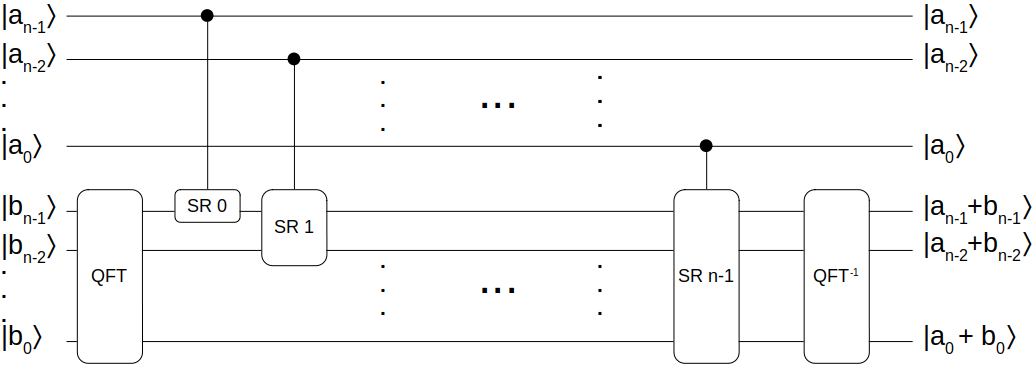
\includegraphics[width=1\textwidth]{qft-adder.png}
  \footnotesize
  \Qcircuit @C=0.35em @R=0.55em {
     & \qw & \gate{\texttt{SR}\;0} & \multigate{3}{\texttt{SR}\;1} & \qw & \qw & \qw & \multigate{5}{\texttt{SR}\;(n-1)} & \qw  \\
      & & & & & \dots & & &  \\
      & \qw & \qw  &  \ghost{\texttt{SR}\; 1} & \qw & \qw & \qw & \ghost{\texttt{SR}\;(n-1)} & \qw \\
      & & & & & & & &  \\
     & & & & & & & &  \\
   & \qw & \qw & \qw & \qw & \qw & \qw & \ghost{\texttt{SR}\;(n-1)}  & \qw 
    }
\end{minipage}
&  
\begin{minipage}{0.25\textwidth}
  \footnotesize
  \Qcircuit @C=0.25em @R=0.35em {
    & \qw & \multigate{3}{(x-a)_n} & \qw \\
    & \vdots & & \\
    & & & \\
    & \qw & \ghost{(x+a)_n} & \qw \\
    }
  \end{minipage}
&
\begin{minipage}{.45\textwidth}
% 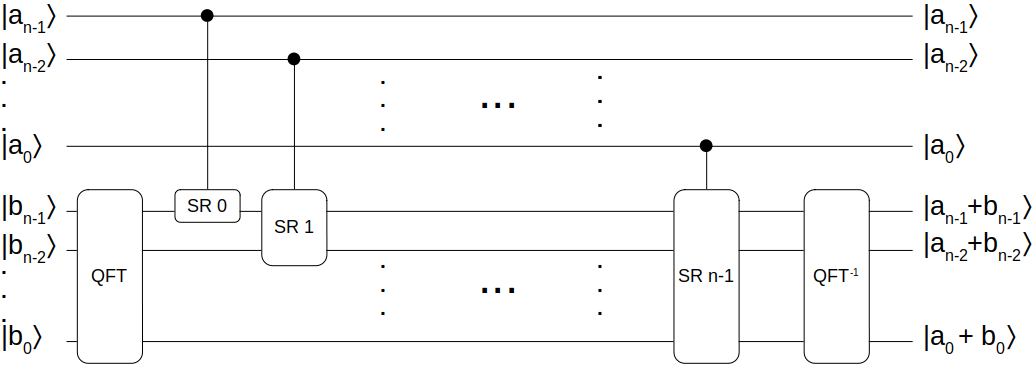
\includegraphics[width=1\textwidth]{qft-adder.png}
  \footnotesize
  \Qcircuit @C=0.35em @R=0.55em {
    & \qw & \multigate{5}{\texttt{SR}^{-1} (n-1)} & \qw & \qw & \qw & \multigate{3}{\texttt{SR}^{-1} 1} & \gate{\texttt{SR}^{-1} 0} & \qw \\
    &     &                                  &     & \dots &   &                              &                      &   \\
    & \qw & \ghost{\texttt{SR}^{-1} (n-1)}        & \qw & \qw   & \qw & \ghost{\texttt{SR}^{-1} 1} & \qw & \qw  \\
      & & & & & & & &  \\
     & & & & & & & &  \\
    & \qw & \ghost{\texttt{SR}^{-1} (n-1)} & \qw & \qw & \qw & \qw & \qw & \qw 
    }
\end{minipage}
\end{tabular}
\caption{Addition/subtraction circuits are inverses}
\label{fig:circuit-add-sub}
\end{figure}

\oqasm programs are easily invertible, as shown by the rules in \Cref{fig:exp-reversed-fun}.
This inversion operation is useful for constructing quantum oracles; for example, the core logic in the QFT-based subtraction circuit is just the inverse of the core logic in the addition circuit (\Cref{fig:exp-reversed-fun}).
This allows us to reuse the proof of addition in the proof of subtraction.
The inversion function satisfies the following properties:

 \begin{theorem}\label{thm:reversibility}\rm[Type reversibility]
    For any well-typed program $\instr$, such that $\Sigma; \Omega \vdash \instr \triangleright \Omega'$, its inverse $\instr'$, where $\instr \xrightarrow{\text{inv}} \instr'$, is also well-typed and we have $\Sigma;\Omega' \vdash \instr' \triangleright \Omega$. Moreover, $\llbracket \instr ; \instr' \rrbracket \varphi=\varphi$.
 \end{theorem}


\end{document}
